% =====================================================================
%  Mini Project Report -- Group 86
%  Dynamic Timetable Monitoring System
%  Based on the SPIT ESE report template (synopsis.tex).
%  Build:  latexmk -pdf 86_Dynamic_Timetable_Monitoring_System.tex
%     or:  pdflatex x3 (for the lists and cross-references)
% =====================================================================
\documentclass[12pt,oneside,a4paper]{article}
\usepackage{epsfig}
\usepackage{cite}
\usepackage{geometry}
\geometry{left=20mm,right=20mm,top=20mm,bottom=50mm}

\usepackage[T1]{fontenc}
\usepackage[utf8]{inputenc}
\usepackage{lmodern}
\usepackage{graphicx}
\usepackage{float}
\usepackage{amsmath,amssymb}
\usepackage{array,booktabs,tabularx,longtable,multirow,makecell}
\usepackage[table]{xcolor}
\usepackage{caption}
\usepackage{subcaption}
\usepackage{enumitem}
\usepackage{setspace}
\usepackage{adjustbox}
\usepackage{tikz}
\usetikzlibrary{shapes.geometric,shapes.multipart,shapes.misc,arrows.meta,positioning,fit,calc,backgrounds}
\usepackage{pgfplots}
\pgfplotsset{compat=1.18}
\usepackage{algorithm}
\usepackage{algpseudocode}
\usepackage{listings}
\usepackage{titlesec}
\usepackage{tocloft}
\usepackage{fancyhdr}
\usepackage{microtype}
\usepackage[hidelinks]{hyperref}
\usepackage{xurl}

% =====================================================================
%  Project details used on the cover, certificates, declaration and
%  headers. Edit ONLY this file to change names, UIDs or the guide.
%  (Items marked TO FILL must be completed by the group.)
% =====================================================================
\newcommand{\GroupNo}{86}
\newcommand{\ProjectTitle}{Dynamic Timetable: A Role-Based Timetable Monitoring System with Automated Timetable Extraction and Natural-Language Queries}
\newcommand{\ProjectShortTitle}{Dynamic Timetable Monitoring System}

% ---- Group members (name, UID) --------------------------------------
\newcommand{\StudentA}{Shivam Mulani}
\newcommand{\UIDA}{2024XXXXXX}          % TO FILL
\newcommand{\StudentB}{Member 2 Name}   % TO FILL
\newcommand{\UIDB}{2024XXXXXX}          % TO FILL
\newcommand{\StudentC}{Member 3 Name}   % TO FILL
\newcommand{\UIDC}{2024XXXXXX}          % TO FILL
\newcommand{\StudentD}{Member 4 Name}   % TO FILL (delete the 4th row in the
\newcommand{\UIDD}{2024XXXXXX}          % title, declaration and poster if the group has 3 members)

% ---- Guide ----------------------------------------------------------
\newcommand{\GuideName}{Prof. Guide Name}   % TO FILL

% ---- Institute ------------------------------------------------------
\newcommand{\Department}{Department of Computer Engineering}
\newcommand{\Programme}{T.E. Computer Engineering}
\newcommand{\Semester}{Semester V}
\newcommand{\CourseName}{Mini Project}
\newcommand{\AcademicYear}{2026--27}
\newcommand{\HODName}{Dr. HOD Name}         % TO FILL (Head, Computer Engineering)
\newcommand{\PrincipalName}{Dr. B. N. Chaudhari}
\newcommand{\RepoURL}{https://github.com/shivammulani-24/Dynamic_Timetable}


% ---------- look & feel ----------------------------------------------
\setstretch{1.15}
\setlength{\emergencystretch}{3em}
\setlength{\parskip}{4pt}
\definecolor{spitblue}{RGB}{0,84,147}
\definecolor{boxfill}{RGB}{232,240,252}
\definecolor{codebg}{RGB}{246,246,246}
\renewcommand{\arraystretch}{1.25}
\captionsetup{font=small,labelfont=bf}
\setlist{itemsep=2pt,topsep=3pt}
\titleformat{\section}{\Large\bfseries}{Chapter \thesection:}{0.6em}{}
\titleformat{\subsection}{\large\bfseries}{\thesubsection}{0.6em}{}
\titleformat{\subsubsection}{\normalsize\bfseries}{\thesubsubsection}{0.6em}{}
\renewcommand{\cftsecpresnum}{}
\setlength{\cftsecnumwidth}{2em}
\numberwithin{figure}{section}
\numberwithin{table}{section}
\renewcommand{\algorithmicrequire}{\textbf{Input:}}
\renewcommand{\algorithmicensure}{\textbf{Output:}}
\lstset{basicstyle=\ttfamily\small,backgroundcolor=\color{codebg},frame=single,
  breaklines=true,columns=fullflexible,keepspaces=true,showstringspaces=false}

\pagestyle{fancy}
\fancyhf{}
\fancyhead[L]{\small \ProjectShortTitle}
\fancyhead[R]{\small Group \GroupNo}
\fancyfoot[C]{\thepage}
\fancyfoot[R]{\small \Department, SPIT}
\renewcommand{\headrulewidth}{0.4pt}

% TikZ styles shared by all diagrams
\tikzset{
  blk/.style={draw=spitblue,thick,rounded corners=3pt,fill=boxfill,align=center,
              minimum height=8mm,inner sep=4pt,font=\small},
  ext/.style={draw,thick,fill=orange!15,align=center,minimum height=9mm,inner sep=4pt,font=\small},
  proc/.style={draw=spitblue,thick,circle,fill=boxfill,align=center,inner sep=2pt,font=\scriptsize,minimum size=19mm},
  store/.style={draw,thick,shape=rectangle,fill=gray!10,align=center,font=\scriptsize,inner sep=3pt,
                append after command={\pgfextra{\draw[thick] (\tikzlastnode.north west)--(\tikzlastnode.north east);}}},
  arr/.style={-{Stealth[length=2.5mm]},thick},
  darr/.style={{Stealth[length=2.5mm]}-{Stealth[length=2.5mm]},thick},
  lbl/.style={font=\scriptsize,fill=white,inner sep=1pt},
  dec/.style={draw=spitblue,thick,diamond,aspect=2.2,fill=yellow!15,align=center,font=\scriptsize,inner sep=1pt},
  term/.style={draw=spitblue,thick,rounded rectangle,fill=green!10,align=center,font=\small,minimum height=7mm},
}

\newcommand{\stick}{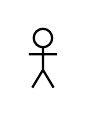
\begin{tikzpicture}[thick,scale=0.9]\draw (0,0.5) circle (0.13); \draw (0,0.37)--(0,0.05) (-0.2,0.27)--(0.2,0.27) (0,0.05)--(-0.15,-0.2) (0,0.05)--(0.15,-0.2);\end{tikzpicture}}
\begin{document}

\begin{titlepage}
\vspace*{0.025cm}
{\centering
{\Large\textbf{\ProjectTitle}}\\
\vspace{0.55cm}
submitted in partial fulfillment of the requirement\\
for the \CourseName{} (\Semester) of\\\vspace{0.45cm}
{\large\textbf{Third Year Bachelor of Technology}}\\
in \\
{\large\textbf{Computer Engineering}}\\
\vspace{0.45cm}
by\\
\vspace{0.4cm}
\renewcommand{\arraystretch}{1.1}
\begin{tabular}{ll}
{\large\textbf{\StudentA}} & {\large \UIDA}\\
{\large\textbf{\StudentB}} & {\large \UIDB}\\
{\large\textbf{\StudentC}} & {\large \UIDC}\\
{\large\textbf{\StudentD}} & {\large \UIDD}\\
\end{tabular}\\
\vspace{0.45cm}
\textbf{Group No. \GroupNo}\\
\vspace{0.35cm}
under the guidance of\\
\vspace{0.3cm}
{\large\textbf{\GuideName}}\\
\begin{figure}[h]
\centering

\includegraphics[scale=0.7]{figures/spitlogo.pdf}
\end{figure}
\textbf{\Department}\\
Bharatiya Vidya Bhavan's\\
Sardar Patel Institute of Technology\\
(Autonomous Institute Affiliated to University of Mumbai)\\
Munshi Nagar, Andheri-West, Mumbai-400058\\
University of Mumbai\\
Academic Year \AcademicYear\par}
\end{titlepage}

\pagenumbering{roman}
\thispagestyle{empty}
\vspace*{0.2cm}
\begin{center}
\large\textbf{Certificate}
\end{center}
\vspace{0.8cm}
This is to certify that the Mini Project entitled ``\textbf{\ProjectTitle}'' by
\textbf{\StudentA{} (\UIDA)}, \textbf{\StudentB{} (\UIDB)} and \textbf{\StudentC{} (\UIDC)}
(Group No.\ \GroupNo) is a bonafide work carried out under the guidance of
\textbf{\GuideName} and is approved for the partial fulfillment of the \CourseName{} of
\Programme{} (\Semester), Academic Year \AcademicYear, of the University of Mumbai.\\
\vspace{0.6cm}
\begin{center}
\textbf{Certified by}
\end{center}
\vspace{1.0cm}

\noindent\begin{tabular*}{\textwidth}{@{}l@{\extracolsep{\fill}}r@{}}
\textbf{\GuideName} & \textbf{\HODName}\\
Project Guide & Head of Department\\
\end{tabular*}

\vspace{1.0cm}
\begin{center}
\textbf{\PrincipalName}\\
\textbf{Principal}
\end{center}

\begin{center}

\includegraphics[scale=0.5]{figures/spitlogo.pdf}
\end{center}
\begin{center}
\textbf{\Department}\\
Bharatiya Vidya Bhavan's\\
Sardar Patel Institute of Technology\\
(Autonomous Institute Affiliated to University of Mumbai)\\
Munshi Nagar, Andheri(W), Mumbai-400058\\
University of Mumbai\\
Academic Year \AcademicYear\\
\end{center}
\newpage

\thispagestyle{empty}
\vspace*{0.2cm}
\begin{center}
\large\textbf{Approval Certificate}
\end{center}
\vspace{1.5cm}
This is to certify that the Mini Project entitled ``\textbf{\ProjectTitle}'' by \StudentA, \StudentB,
\StudentC{} and \StudentD{} (Group No.\ \GroupNo) is approved for the partial fulfillment of the
\CourseName{} of \Programme{} (\Semester), Academic Year \AcademicYear, of the University of Mumbai.

\vspace{2.2cm}
\noindent\begin{tabular*}{\textwidth}{@{}l@{\extracolsep{\fill}}l@{}}
\textbf{Project Guide} & \textbf{External Examiner}\\[1.8cm]
\textbf{(signature)} & \textbf{(signature)}\\[0.9cm]
\textbf{Name:} & \textbf{Name:}\\[0.9cm]
\textbf{Date:} & \textbf{Date:}\\[2.2cm]
\textbf{Head of Department} & \textbf{Principal}\\
\end{tabular*}

\vspace{2cm}
\begin{center}
\textbf{Seal of the Institute}
\end{center}
\newpage

\section*{\centering{Declaration}}
\thispagestyle{plain}
\vspace{2.5cm}
We wish to state that the work embodied in this report titled ``\ProjectTitle'' forms our own
contribution to the work carried out under the guidance of \GuideName{} at the Sardar Patel Institute
of Technology. We declare that this written submission represents our ideas in our own words and
where others' ideas or words have been included, we have adequately cited and referenced the original
sources. We also declare that we have adhered to all principles of academic honesty and integrity and
have not misrepresented or fabricated or falsified any idea/data/fact/source in our submission.

\vspace{3cm}
\noindent\begin{tabular*}{\textwidth}{@{}l@{\extracolsep{\fill}}l@{\extracolsep{\fill}}l@{\extracolsep{\fill}}l@{}}
\textbf{\StudentA} & \textbf{\StudentB} & \textbf{\StudentC} & \textbf{\StudentD}\\[1.6cm]
(signature) & (signature) & (signature) & (signature)\\[0.5cm]
UID: \UIDA & UID: \UIDB & UID: \UIDC & UID: \UIDD\\
\end{tabular*}

\vspace{2cm}
\noindent Date: \hfill Place: Mumbai
\newpage

\section*{\centering{Acknowledgement}}
\addcontentsline{toc}{section}{Acknowledgement}
\vspace{1cm}
We express our sincere gratitude to our project guide, \textbf{\GuideName}, for the constant
guidance, the suggested improvements and the scenario-based challenges that shaped this project,
and for reviewing our work at every stage.

We are thankful to \textbf{\HODName}, Head of the \Department, and to \textbf{\PrincipalName},
Principal, Sardar Patel Institute of Technology, for providing the facilities and the encouraging
environment in which this mini project was carried out.

We thank the faculty members of the \Department{} whose teaching of Software Engineering, Database
Management Systems, Operating Systems, Computer Networks, Data Structures and Analysis of Algorithms
formed the foundation of this work, and the department office for making the official class
timetable available, which we used as the real-world test document for the system.

Finally, we thank our families and friends for their support and for patiently testing the app on
their phones.

\vspace{2cm}
\noindent\begin{tabular*}{\textwidth}{@{}l@{\extracolsep{\fill}}l@{\extracolsep{\fill}}l@{\extracolsep{\fill}}l@{}}
\StudentA & \StudentB & \StudentC & \StudentD\\
\end{tabular*}
\newpage

\section*{\centering{Abstract}}
\addcontentsline{toc}{section}{Abstract}
\vspace{0.5cm}
In most colleges the class timetable is published as a multi-page PDF that every student and teacher
has to read by hand. Finding the next class, a free room or a teacher's location means scanning dense
grids full of abbreviations, lab sub-groups and footnote legends, and every revision of the timetable
has to be re-checked manually. Clashes between teachers or rooms are usually discovered only when they
happen.

This mini project builds \textbf{Dynamic Timetable}, a role-based timetable monitoring system made of
a cross-platform mobile and web app (React Native with Expo) and a central back end (Python FastAPI
and PostgreSQL). The Admin uploads the official timetable as PDF, Excel, Word or a photo. A
background worker extracts every class cell with geometry-aware table parsing and OCR, expands the
per-page legends, separates lab sub-groups, validates times and flags anything uncertain for review.
Students, professors, the HOD and the Principal then see a dashboard (current class, next class,
free periods) and can ask questions in plain English such as ``Do I have classes after lunch on
Tuesday?'', ``How many labs do I have this week?'' or ``Which day is my busiest?''. A deterministic
compositional planner turns each question into a typed query plan (an operation such as list, count,
first/last, total hours or day-wise summary, combined with filters, a date or week, a time window and
an ordering), which the server compiles into parameterised queries with the user's role scope added.
It never generates SQL from text and cannot be talked into reading other users' data. Institutional and personal timetables are
kept strictly separate, and the system automatically detects professor, room and batch clashes.

On the college's real 10-page timetable PDF the system extracted 453 class entries, of which 452
were verified automatically; the one remaining entry has no time printed in the PDF. It also reported
exactly the two genuine clashes present in the document. The work is supported by 174 automated
back-end tests, 20 mobile unit tests and end-to-end browser tests (24/24 and 21/21 passing).
Measured single-user search latency was about 37--47~ms (median) on a 4-core development machine.
The system has been deployed as a free online demo. Its limitations are that it has not been load
tested on production hardware, push notifications need a store build, and extraction accuracy has
not yet been measured against a hand-labelled ground truth.

\vspace{0.5cm}
\noindent\textbf{Keywords:} timetable extraction, table recognition, OCR, natural-language interface,
intent classification, role-based access control, conflict detection, React Native, FastAPI,
PostgreSQL.
\newpage


\newpage
\phantomsection\addcontentsline{toc}{section}{Contents}
\tableofcontents
\newpage
\phantomsection\addcontentsline{toc}{section}{List of Figures}
\listoffigures
\newpage
\phantomsection\addcontentsline{toc}{section}{List of Tables}
\listoftables
\newpage
\section*{List of Abbreviations}
\addcontentsline{toc}{section}{List of Abbreviations}
\begin{longtable}{@{}p{0.2\textwidth}p{0.75\textwidth}@{}}
\toprule
\textbf{Abbreviation} & \textbf{Full form}\\
\midrule
\endhead
ACID & Atomicity, Consistency, Isolation, Durability\\
API & Application Programming Interface\\
APNI Leap & Department framework for applying Semester I--IV engineering concepts in projects\\
CRUD & Create, Read, Update, Delete\\
CSV & Comma-Separated Values\\
DFD & Data Flow Diagram\\
DOCX / XLSX & Office Open XML Word document / spreadsheet\\
E2E & End-to-End (testing)\\
ER & Entity--Relationship\\
FK / PK & Foreign Key / Primary Key\\
FR / NFR & Functional / Non-Functional Requirement\\
HOD & Head of Department\\
HTTP(S) & Hypertext Transfer Protocol (Secure)\\
IANA & Internet Assigned Numbers Authority (time-zone database)\\
IDOR & Insecure Direct Object Reference\\
JSON & JavaScript Object Notation\\
JWT & JSON Web Token\\
KPI & Key Performance Indicator\\
LLC & Liberal Learning Course (co-curricular slot in the college timetable)\\
NL / NLP & Natural Language / Natural-Language Processing\\
OCR & Optical Character Recognition\\
ORM & Object--Relational Mapper\\
PDF & Portable Document Format\\
PWA & Progressive Web App\\
RBAC & Role-Based Access Control\\
REST & Representational State Transfer\\
SDK & Software Development Kit\\
SQL & Structured Query Language\\
SRS & Software Requirements Specification\\
TT & Timetable\\
UI / UX & User Interface / User Experience\\
UID & Unique Identification (student identity number)\\
UML & Unified Modeling Language\\
\bottomrule
\end{longtable}


\newpage
\pagenumbering{arabic}
\section{Introduction and Problem Definition}

\subsection{Project Background}
Every semester the timetable committee of an engineering college publishes the class timetable as a
multi-page PDF: one grid per division for each of F.E., S.E., T.E., B.E.\ and M.Tech., with days as
rows, time slots as columns and, below each grid, a legend that expands abbreviations such as
\texttt{DBMS}, \texttt{KKD} or \texttt{LLC}. A single cell may contain a subject, a teacher code, a
room number and, for practical sessions, four stacked lab sub-groups (\texttt{A1}--\texttt{A4}), each
with its own teacher and laboratory. Electives, combined B.E.\ classes, ``Tentative'' sections and
``W.E.F.'' (with-effect-from) dates are written in free text around the grid.

Students and teachers read this document by hand many times a day: to find the next lecture, to see
whether a lab is in 606 or 607, to locate a teacher, or to look for an empty room for a make-up
lecture. When a revised PDF is circulated, everyone has to compare it with the old one manually.
Clashes, for example one professor assigned to two rooms at the same time, are usually noticed only
when they happen in the corridor. Generic calendar apps do not help, because nobody types 450 classes
into a calendar, and timetable-generation software is used only by the committee that creates the
timetable, not by the people who follow it.

\subsection{Problem Statement}
\begin{quote}
\emph{Design and implement a system that converts a college's published timetable (PDF, spreadsheet,
Word file or photograph) into verified structured data, keeps every version as an auditable archive,
detects scheduling clashes, and lets each user (student, professor, HOD, Principal or administrator)
get correct, role-appropriate answers to everyday timetable questions on a mobile phone or laptop,
including questions typed in plain English, without ever exposing one user's personal data to
another.}
\end{quote}

The difficulties with the existing approach are:
\begin{enumerate}
\item \textbf{Unstructured source.} The timetable exists only as a visually formatted document.
      Merged cells, stacked lab rows, page-specific legends, inconsistent time labels (for example a
      row printed as ``12.15--1.15'' without a.m./p.m.) and scanned pages make automatic reading hard.
\item \textbf{Manual lookup.} Answering ``Where is my next class?'' requires locating the right
      page, row, column and lab sub-group, and expanding the legend codes.
\item \textbf{No conflict visibility.} Teacher, room and batch overlaps are not checked mechanically.
\item \textbf{Version confusion.} Old and new PDFs circulate together; it is unclear which one is
      official.
\item \textbf{Privacy.} Students may also want to keep a personal timetable (tuition, coaching),
      which must never be visible to the college administration.
\end{enumerate}

\subsection{Motivation}
The problem affects every member of the college every working day. A typical department timetable
has more than 450 class entries across ten pages, and each of several hundred students and about 50 faculty
members consults it several times a day. Even saving one minute per lookup saves hundreds of
person-hours per semester. More importantly, an automatically checked timetable removes clashes
\emph{before} the semester starts. The project also gave us the opportunity to apply, in one
realistic system, almost every core subject of the first four semesters: data structures and
algorithms in the parser and query engine, DBMS in the schema and transactions, operating-system
concepts in the background worker and concurrency control, computer networks in the client--server
API, and software engineering throughout.

\subsection{Objectives}
The objectives were defined to be specific and measurable:
\begin{enumerate}[label=\textbf{O\arabic*.}]
\item Extract class entries from the college's real timetable PDF with at least 95\% of entries
      verified automatically, and flag every uncertain value for human review instead of guessing.
\item Support at least five input formats (PDF, scanned PDF/photo via OCR, XLSX/CSV, DOCX) through one
      common pipeline.
\item Provide role-based dashboards (current class, next class, free periods) for five roles:
      Student, Professor, HOD, Principal and Admin, with server-side enforcement of permissions.
\item Answer everyday questions typed in English through a deterministic engine covering at least
      25 question types, with clarification instead of guessing when a question is ambiguous.
\item Detect professor, room and batch clashes automatically and report only genuine clashes.
\item Keep institutional and personal timetables strictly separate, with complete version history.
\item Achieve a median search response time below 300~ms for a single user on modest hardware, with
      no incorrect answers under concurrent use.
\item Run on Android, iPhone and laptop browsers from one code base, and deploy a free online demo.
\item Back the system with automated tests (unit, integration, end-to-end) with 100\% of tests passing
      before every commit.
\end{enumerate}

\subsection{Scope of the Project}
\paragraph{Features included.}
Timetable upload and extraction (PDF, scanned PDF, JPG/PNG, XLSX, XLS, CSV, DOCX, DOC); validation,
review and auditable correction; archive of all versions with one official (primary) timetable;
activation notifications; conflict detection; role dashboards; weekly timetable view; natural-language
search (30 intents); free-room and professor-availability search; personal timetables; academic-year
promotion of students; administrator master data (departments, batches, courses, rooms, users,
aliases); audit log.

\paragraph{Features outside the scope.}
Automatic \emph{generation} or optimisation of a timetable (the committee still creates it);
attendance; live location tracking of teachers (the system reports only the \emph{scheduled} room);
exam timetables; integration with the college ERP; free-form chat with a large language model.

\paragraph{Intended users.}
Students, professors, Heads of Department, the Principal and the timetable administrator.

\paragraph{Operating environment.}
Android and iOS phones (as an installable app or a home-screen web app), laptop browsers (Chrome,
Edge, Safari, Firefox) and a Linux server or cloud container running Python 3.12+ and PostgreSQL 14+.

\paragraph{Expected scale.}
One institute: about 2{,}000--3{,}000 users, 50--100 batches, 500--1{,}000 class entries per
timetable, a few timetable versions per semester and short bursts of concurrent use around lecture
changes.

\subsection{Proposed Solution}
The proposed system (Figure~\ref{fig:arch}) has three parts:
\begin{enumerate}
\item \textbf{An extraction pipeline} that converts any supported file into a common \emph{grid}
      model, recognises sections, time rows, lab sub-groups, legends and breaks, validates every entry
      and assigns it a status: \textsc{Verified}, \textsc{Unverified}, \textsc{Incomplete} or
      \textsc{Rejected}.
\item \textbf{A central back end} (FastAPI + PostgreSQL) that stores timetables as archives, enforces
      role-based access on every request, detects conflicts, and answers questions through a
      rule-based natural-language engine with a fixed registry of 30 intents (Q01--Q30) and 22
      parameterised query templates (QT01--QT22).
\item \textbf{A cross-platform app} (React Native/Expo) with role dashboards, a weekly view, an
      ``Ask'' screen, archives, uploads, review screens and administrator tools.
\end{enumerate}

\subsection{Novelty and Originality}
\begin{itemize}
\item \textbf{End-to-end from the real document.} Most student timetable apps expect the timetable to
      be typed in. This system reads the college's actual PDF, including its specific conventions:
      stacked lab sub-groups, page-wise legends, the 12:15 ``noon'' row, combined B.E.\ electives and
      co-curricular LLC slots with no teacher or room.
\item \textbf{Honest uncertainty.} Instead of silently guessing, every entry carries a verification
      status, the raw source text and its page. Ambiguous a.m./p.m.\ is never corrected silently.
\item \textbf{Safe natural-language queries.} Questions are mapped to a closed registry of intents and
      parameterised templates. The engine never builds SQL from user text, which makes it immune to
      prompt or SQL injection by construction and makes every answer reproducible.
\item \textbf{Strict domain separation.} Institutional and personal data live in separate tables;
      the code cannot even express a query that unions them.
\item \textbf{Clash detection with intent awareness.} Parallel lab sub-groups and elective options are
      recognised as intended overlaps, so only genuine clashes are reported (542 raw overlaps reduced
      to the 2 genuine clashes in the real PDF).
\end{itemize}

\subsection{Feasibility Analysis}
\paragraph{Technical feasibility.}
All components use mature open-source software: PyMuPDF for PDF geometry, Tesseract for OCR,
FastAPI and SQLAlchemy for the API, PostgreSQL for storage and Expo for the app. The team had
working knowledge of Python, SQL and JavaScript from earlier semesters. The riskiest part, parsing
the real PDF, was prototyped first and proved feasible (Chapter~10).

\paragraph{Economic feasibility.}
The software stack is free. Development used personal laptops. The online demo runs on Render's free
tier (free web service and a free PostgreSQL database), so the total cost is
\textbf{Rs.~0}. Production hosting for real students is estimated at about
US\$7--25 per month (a small always-on instance and a managed database).

\paragraph{Operational feasibility.}
Users need only a browser or the Expo/installed app. The Admin's workflow (upload, review,
activate) mirrors the existing manual process, and the system never changes the official timetable
without explicit activation.

\paragraph{Time and resource feasibility.}
The work was planned over one semester in phases (requirements, back-end foundation, extraction,
query engine, app, testing, deployment), which fits the mini-project timeline. Section~7.8 shows the
commit history.

\subsection{Social Relevance and Practical Applications}
\begin{itemize}
\item Students, especially first-years and students who switch divisions or electives, can find the
      right class, lab and room instantly, reducing late arrivals and confusion.
\item Faculty can check their own schedule and free periods, and find free rooms for extra lectures.
\item The HOD and Principal get a clash report and a view of room usage, which supports better use of
      classrooms and laboratories, a scarce resource in Indian colleges.
\item The archive gives a transparent record of which timetable was official on which date.
\item The approach transfers to schools, coaching institutes, hospitals (duty rosters) and any
      organisation that publishes grid-style schedules as PDFs.
\item Accessibility: the plain-English ``Ask'' screen, large tap targets and dark mode help users who
      find dense PDF grids hard to read.
\end{itemize}

\subsection{Success Criteria and Key Performance Indicators}
Table~\ref{tab:kpi} lists the KPIs fixed before testing. Chapter~9 (Section~9.10) compares the measured values with
these targets.

\begin{table}[H]
\centering
\caption{Key performance indicators and targets}
\label{tab:kpi}
\small
\begin{tabularx}{\textwidth}{@{}p{2.8cm}X p{3.0cm}X@{}}
\toprule
\textbf{KPI} & \textbf{Definition} & \textbf{Target} & \textbf{Measurement method}\\
\midrule
Extraction verification rate & Verified class entries / all class entries on the real PDF & $\geq 95\%$ & Seed run on the real PDF; regression test\\
False clash reports & Reported conflicts that are not genuine clashes & 0 & Manual check of every reported conflict against the PDF\\
Response time & Median server time per NL search, single user & $< 300$ ms & Timestamped client measurement, 50 requests per query type\\
Throughput & Searches served per second with 4 API workers & $\geq 30$ req/s & Multi-threaded load test (Section 8.6)\\
Reliability & Correct responses / total requests under concurrency & 100\% & Load test, response status check\\
Functional correctness & Passed / total automated tests & 100\% & pytest, Jest, Playwright\\
Extraction time & Time to extract the 10-page real PDF & $< 10$ s & Timed pipeline run (median of 5)\\
Resource usage & Memory of one API worker; database size for one timetable & $< 300$ MB; $< 50$ MB & \texttt{ps}, \texttt{pg\_database\_size}\\
Coverage of questions & Number of supported question types (intents) & $\geq 25$ & Intent registry and its tests\\
\bottomrule
\end{tabularx}
\end{table}

\newpage

\section{Literature Review and Study of Existing Systems}

\subsection{Study of Existing Systems}
\paragraph{Manual process (current practice).}
The timetable committee prepares the timetable in a spreadsheet or word processor and circulates a
PDF by e-mail, on WhatsApp groups and on notice boards. Users read it by hand. The process costs
nothing and everyone understands it, but it supports no search, no personalisation, no clash
checking and no version control.

\paragraph{Timetable generation software: FET, UniTime and aSc Timetables.}
FET~\cite{fet} is a free, open-source timetable generator. UniTime~\cite{unitime} is an open-source,
web-based university course timetabling and student scheduling system. aSc Timetables~\cite{asc} is a
commercial school timetable generator. These tools solve the \emph{construction} problem: they
assign events to time slots and rooms under hard and soft constraints, and they export the result
as printable grids. They are used by the committee, not by students. They do not read an existing
PDF, and their published output is again a static document.

\paragraph{PDF table-extraction tools: Tabula and Camelot.}
Tabula~\cite{tabula} and Camelot~\cite{camelot} extract tables from text-based PDFs into CSV. They
handle ruled tables well, but they return raw cell strings: they do not understand time rows, lab
sub-groups, legends, merged two-hour cells or a.m./p.m.\ ambiguity, and they do not work on scanned
images without separate OCR.

\paragraph{General calendar apps: Google Calendar and Outlook.}
Calendar apps offer reminders and sharing, but every event must be entered by hand or imported from
an iCalendar file that the college does not publish. They have no notion of roles, batches,
rooms or room availability.

\paragraph{College ERP / LMS timetable modules.}
ERP products and learning-management systems often include a timetable module, but the data must be
keyed in by staff, the modules are usually closed and licensed per student, and they rarely offer
free-room search, clash reports or natural-language queries.

\paragraph{Natural-language interfaces built on large language models.}
Recent assistants translate questions into SQL with large language models (text-to-SQL). They are
flexible, but answers are not reproducible, they can produce plausible but wrong queries, and they
are vulnerable to prompt-injection attacks that lead to SQL injection~\cite{pedro2023,greshake2023}.

\subsection{Review of Research Papers and Technical Resources}
Table~\ref{tab:litreview} summarises the papers and technical resources reviewed, grouped by
theme. The rest of this section discusses the most important ones.

\paragraph{Timetabling.}
Schaerf's survey~\cite{schaerf1999} classifies school, course and examination timetabling problems
and the search techniques used to solve them. Burke and Petrovic~\cite{burke2002} review research
directions in university timetabling, including constraint-based, meta-heuristic and hybrid methods,
and point out the gap between research prototypes and real institutional data. Lewis~\cite{lewis2008}
surveys meta-heuristics for university course timetabling and separates hard constraints (no clashes
of teachers, rooms or student groups) from soft ones. These works define the clash model we
\emph{check} after publication (professor, room and batch overlap), but they all assume that the
timetable is created by the software. None of them addresses reading an already published timetable.

\paragraph{Table recognition and OCR.}
Zanibbi, Blostein and Cordy~\cite{zanibbi2004} survey table recognition and describe the pipeline of
table detection, structure recognition (rows, columns, spanning cells) and interpretation. They note
that interpretation is domain specific. Kieninger and Dengel~\cite{kieninger1998} (T-Recs) recognise
tables from word bounding boxes without ruling lines. We use the same idea in our geometric
fallback, which rebuilds columns from whitespace gutters. The ICDAR 2013 table competition~\cite{gobel2013}
established standard evaluation of table location and structure, showing that cell-structure recovery
remains error-prone and motivating our per-cell verification status. Smith~\cite{smith2007} describes
the Tesseract OCR engine (adaptive classifier, line finding and word recognition) used for scanned
pages and photographs. PyMuPDF~\cite{pymupdf} provides text with coordinates and ruled-table detection
that preserves merged-cell spans.

\paragraph{Natural-language interfaces to databases.}
Androutsopoulos, Ritchie and Thanisch~\cite{androutsopoulos1995} review classical natural-language
interfaces to databases (NLIDB), including pattern-matching, syntax-based and semantic-grammar
systems. They note that a narrow domain allows simple, reliable pattern-based interpretation. Seq2SQL~\cite{zhong2017}
and the Spider benchmark~\cite{yu2018} show that neural text-to-SQL can generalise across schemas, but
exact-match accuracy on complex queries remains well below 100\%, which is unacceptable when a student
relies on the answer to reach a lab on time. Greshake et~al.~\cite{greshake2023} and Pedro
et~al.~\cite{pedro2023} demonstrate prompt-injection attacks on LLM-integrated applications, including
attacks that turn prompts into SQL injection. These findings led us to a closed intent registry with
parameterised templates instead of generated SQL.

\paragraph{Time intervals and conflicts.}
Allen's interval algebra~\cite{allen1983} defines the thirteen relations between time intervals. Our
clash rule uses the \emph{overlaps/during/equals} family, $a.\mathit{start} < b.\mathit{end} \wedge
b.\mathit{start} < a.\mathit{end}$, with start-inclusive, end-exclusive slots, so consecutive lectures do
not clash.

\paragraph{Security and architecture.}
Sandhu et~al.~\cite{sandhu1996} define role-based access control (RBAC), which underlies our five
roles and their data scopes. JSON Web Tokens are specified in RFC~7519~\cite{rfc7519}. Argon2, the
winner of the Password Hashing Competition, is a memory-hard function resistant to GPU
cracking~\cite{biryukov2016}. The OWASP Top~10~\cite{owasp2021} lists broken access control and
injection among the most critical web risks, and it guided our IDOR and injection controls.
Fielding's REST dissertation~\cite{fielding2000} motivates the stateless resource-oriented API, and
Codd's relational model~\cite{codd1970} with normalisation theory~\cite{silberschatz2019} underlies
the schema. PostgreSQL's \texttt{SELECT \ldots{} FOR UPDATE SKIP LOCKED}~\cite{postgresdocs} lets
several worker processes take jobs from one table without a separate message broker.

\begin{longtable}{@{}p{0.6cm}p{3.6cm}p{5.4cm}p{5.6cm}@{}}
\caption{Summary of reviewed literature and resources}\label{tab:litreview}\\
\toprule
\textbf{\#} & \textbf{Work} & \textbf{Contribution} & \textbf{Relevance / limitation for our problem}\\
\midrule
\endfirsthead
\toprule
\textbf{\#} & \textbf{Work} & \textbf{Contribution} & \textbf{Relevance / limitation for our problem}\\
\midrule
\endhead
1 & Schaerf, 1999~\cite{schaerf1999} & Survey of school, course and exam timetabling formulations and algorithms & Defines clash constraints; assumes timetable is generated, not read\\
2 & Burke \& Petrovic, 2002~\cite{burke2002} & Research directions in university timetabling & Highlights gap between research and real institutional data\\
3 & Lewis, 2008~\cite{lewis2008} & Survey of meta-heuristics for university timetabling; hard vs soft constraints & Hard constraints become our conflict checks\\
4 & Zanibbi et al., 2004~\cite{zanibbi2004} & Survey of table recognition: detection, structure, interpretation & Interpretation is domain specific, so we built a timetable-specific grid parser\\
5 & Kieninger \& Dengel, 1998~\cite{kieninger1998} & T-Recs: tables from word boxes without ruling lines & Basis of our geometric (gutter-based) fallback\\
6 & G\"obel et al., 2013~\cite{gobel2013} & ICDAR 2013 table competition and metrics & Structure recovery is error-prone, so we assign a status to each entry\\
7 & Smith, 2007~\cite{smith2007} & Architecture of the Tesseract OCR engine & OCR for scans/photos; OCR entries capped at \textsc{Unverified}\\
8 & Androutsopoulos et al., 1995~\cite{androutsopoulos1995} & Review of NL interfaces to databases & Narrow domain allows reliable rule-based interpretation\\
9 & Zhong et al., 2017~\cite{zhong2017} & Seq2SQL: neural text-to-SQL with RL & Flexible but not exact; needs training data\\
10 & Yu et al., 2018~\cite{yu2018} & Spider cross-domain text-to-SQL benchmark & Accuracy on complex queries far below 100\%\\
11 & Greshake et al., 2023~\cite{greshake2023} & Indirect prompt injection in LLM-integrated apps & Risk of letting an LLM drive data access\\
12 & Pedro et al., 2023~\cite{pedro2023} & Prompt-to-SQL injection in LLM web apps & Motivates templates instead of generated SQL\\
13 & Allen, 1983~\cite{allen1983} & Interval algebra for temporal reasoning & Formal basis of the overlap/clash rule\\
14 & Sandhu et al., 1996~\cite{sandhu1996} & Role-based access control models & Five roles with data scopes\\
15 & Biryukov et al., 2016~\cite{biryukov2016} & Argon2 memory-hard password hashing & Password storage\\
16 & Fielding, 2000~\cite{fielding2000} & REST architectural style & Stateless JSON API design\\
17 & Codd, 1970~\cite{codd1970} & Relational model of data & Normalised relational schema\\
18 & RFC 7519~\cite{rfc7519}, OWASP Top 10~\cite{owasp2021} & JWT standard; top web security risks & Token format; IDOR and injection controls\\
19 & FET, UniTime, aSc~\cite{fet,unitime,asc} & Timetable generators & Construct timetables; no reading, search or role views\\
20 & Tabula, Camelot, PyMuPDF~\cite{tabula,camelot,pymupdf} & PDF table extraction tools & Raw cells only; no timetable semantics\\
\bottomrule
\end{longtable}

\subsection{Comparative Analysis}
Table~\ref{tab:compare} compares the existing approaches on criteria that matter to the users of a
published college timetable.

\begin{table}[H]
\centering
\caption{Comparison of existing approaches with the proposed system}
\label{tab:compare}
\footnotesize
\setlength{\tabcolsep}{3pt}
\begin{tabular}{@{}p{3.6cm}*{7}{>{\centering\arraybackslash}p{1.6cm}}@{}}
\toprule
\textbf{Criterion} & \textbf{Manual PDF} & \textbf{FET / UniTime / aSc} & \textbf{Tabula / Camelot} & \textbf{Calendar apps} & \textbf{ERP module} & \textbf{LLM text-to-SQL} & \textbf{Proposed}\\
\midrule
Reads published PDF/photo & -- & No & Partly & No & No & No & \textbf{Yes}\\
Timetable semantics (labs, legends) & Human & Yes & No & No & Yes & Depends & \textbf{Yes}\\
Role-based views & No & Limited & No & No & Yes & No & \textbf{Yes (5)}\\
Plain-English questions & No & No & No & Limited & No & Yes & \textbf{Yes (composed plans)}\\
Reproducible, injection-safe answers & -- & -- & -- & -- & Yes & No & \textbf{Yes}\\
Clash detection & No & At creation & No & No & Sometimes & No & \textbf{Yes, after publication}\\
Version archive & Ad hoc & Files & No & No & Sometimes & No & \textbf{Yes, audited}\\
Personal timetable kept private & -- & No & No & Yes & No & No & \textbf{Yes}\\
Cost & Free & Free/Paid & Free & Free & Paid & Paid API & \textbf{Free (open source)}\\
Mobile use & PDF viewer & Limited & No & Yes & Varies & Varies & \textbf{Android, iOS, web}\\
\bottomrule
\end{tabular}
\end{table}

\subsection{Limitations of Existing Systems}
\begin{enumerate}
\item Generators (FET, UniTime, aSc) stop at a printable grid; the people who follow the timetable
      cannot search or personalise it.
\item Generic table extractors do not understand timetable conventions: stacked labs become one
      garbled string, legends are not applied, and times stay ambiguous.
\item Calendars and ERP modules require manual data entry, which is error-prone and is rarely
      repeated when the timetable is revised.
\item No existing tool used by our college detects clashes in the \emph{published} timetable.
\item LLM-based interfaces are not reproducible and introduce injection risks~\cite{pedro2023}.
\end{enumerate}

\subsection{Identified Engineering Gap}
There is no free system that takes the timetable \emph{as the college actually publishes it} and
turns it into trustworthy, role-scoped, searchable data with provenance, clash checks and version
history, while answering everyday questions in plain English safely. The gap is not a better
timetable-construction algorithm. It is the missing link between the published document and its
daily users.

\subsection{Proposed Improvements}
\begin{itemize}
\item A timetable-aware extraction pipeline with geometry, OCR and office adapters feeding one grid
      model, with per-entry provenance and verification status (closes limitations 2 and 3).
\item Admin review, correction and activation with an audited archive (closes limitation 3).
\item Interval-based clash detection that understands parallel lab groups and elective options
      (closes limitation 4).
\item A compositional NL query planner (typed plans compiled into parameterised queries) with clarification instead of guessing
      (closes limitation 5).
\item Role dashboards and a single code base for Android, iOS and the web (closes limitation 1).
\end{itemize}

\newpage

\section{Software Requirements Specification (SRS)}

\subsection{Purpose and Scope of the SRS}
This SRS defines what the Dynamic Timetable system must do (functional requirements) and how well
it must do it (non-functional requirements) for its first release (V1). It is the reference for
design (Chapter~4), implementation (Chapter~7) and testing (Chapter~9): every functional requirement
has an identifier that appears in the test-case table (Section~9.8). The SRS covers the back-end
API, the extraction worker and the cross-platform client; timetable \emph{generation}, attendance and
ERP integration are excluded (Section~1.5).

\subsection{Intended Users and Stakeholders}
\begin{table}[H]
\centering
\caption{Users, stakeholders and their goals}
\label{tab:users}
\small
\begin{tabularx}{\textwidth}{@{}p{3cm}X@{}}
\toprule
\textbf{User / stakeholder} & \textbf{Goals and permissions}\\
\midrule
Student & See own batch and lab-group classes, next class, free periods, free rooms; view and ask about any batch, teacher, room or clash (viewing is open); keep a private personal timetable.\\
Professor & See own teaching schedule and free periods; find rooms; locate colleagues' \emph{scheduled} room.\\
HOD & Everything a professor can do, plus the Conflicts screen. (Clashes, floor activity and room usage can be asked about by anyone.)\\
Principal & College-wide read access to dashboards, clashes and room usage.\\
Admin (timetable coordinator) & Upload, review, correct and activate official timetables; manage master data, users, roles and promotions; read the audit log. Cannot read anyone's personal timetable.\\
Timetable committee & Benefits from automatic clash detection before publishing.\\
College management & Transparent version history; better room utilisation.\\
\bottomrule
\end{tabularx}
\end{table}

\subsection{Overall Product Description}
\paragraph{System environment.}
A client--server system. Clients are the Expo/React Native app (Android, iOS) and the same app compiled
for the web (laptop browsers, home-screen web app). The server is a stateless FastAPI application
behind HTTPS, a PostgreSQL database, a background worker for extraction and private file storage for
uploaded originals.

\paragraph{Major functions.}
(1) authentication and role-based authorisation; (2) timetable upload, extraction, validation, review,
correction and activation; (3) archives and primary (default) selection per domain; (4) dashboards and
weekly views; (5) natural-language search; (6) conflict detection; (7) academic administration
(departments, years, batches, courses, rooms, users, promotion); (8) notifications and audit.

\paragraph{Dependencies.}
PostgreSQL 14+ (tested 16); Tesseract OCR for scans/photos; LibreOffice only for legacy
\texttt{.xls}/\texttt{.doc}; an SMTP server for e-mail (optional; without it the Admin hands out
activation codes); Expo push service for push notifications (store builds only).

\paragraph{Operating conditions.}
Times are stored as local wall-clock times of the institute; ``now'' is computed in the user's IANA
time zone (default \texttt{Asia/Kolkata}). Week start, lunch boundary and working hours are configured
by the Admin and never assumed.

\subsection{Functional Requirements}
Table~\ref{tab:fr} lists the functional requirements. For each one it gives the input, the expected
processing and output, and the acceptance criterion used in testing.

\begingroup\small
\begin{longtable}{@{}p{1.1cm}p{3.4cm}p{6.2cm}p{4.9cm}@{}}
\caption{Functional requirements}\label{tab:fr}\\
\toprule
\textbf{ID} & \textbf{Requirement} & \textbf{Input $\rightarrow$ processing $\rightarrow$ output} & \textbf{Acceptance criterion}\\
\midrule
\endfirsthead
\toprule
\textbf{ID} & \textbf{Requirement} & \textbf{Input $\rightarrow$ processing $\rightarrow$ output} & \textbf{Acceptance criterion}\\
\midrule
\endhead
FR-01 & Sign-in with college e-mail and password & E-mail, password $\rightarrow$ Argon2id verify, account-status check, rate limit $\rightarrow$ 15-min access JWT + rotating refresh token & Wrong e-mail or password gives the same generic error; suspended account refused\\
FR-02 & Five roles enforced on the server & Request + token $\rightarrow$ roles loaded from \texttt{USER\_ROLE} on every request $\rightarrow$ allowed / 403 & No endpoint trusts a client-sent role; role change invalidates old tokens\\
FR-03 & Upload a timetable (PDF, image, XLSX/XLS, CSV, DOCX/DOC) & File $\rightarrow$ extension allow-list, content-signature check, size/page limits, private storage, SHA-256, job queued $\rightarrow$ archive record (\textsc{Queued}) & Upload never changes the primary timetable; retries with the same request id are idempotent\\
FR-04 & Extract class entries & Stored file $\rightarrow$ worker: page inspection, table/OCR extraction, sections, time rows, cell parsing, legend expansion, mapping $\rightarrow$ entries with provenance and status & Real college PDF: $\geq 95\%$ of class entries \textsc{Verified}; nothing guessed silently\\
FR-05 & Validate and classify the timetable & Entries $\rightarrow$ checks (missing fields, duplicates, time consistency, overlaps) $\rightarrow$ \textsc{Ready} / \textsc{Needs Review} / \textsc{Unusable} / \textsc{Failed} & Unusable timetables cannot become primary\\
FR-06 & Review and correct entries & Admin edits $\rightarrow$ before/after snapshot in \texttt{ENTRY\_CORRECTION}, audit row $\rightarrow$ corrected entry & Original value always recoverable; entry becomes \textsc{Verified} only by explicit reviewer action\\
FR-07 & Activate the official timetable & Admin action $\rightarrow$ settings row locked, primary switched, version incremented, users notified $\rightarrow$ new primary & Concurrent activations serialise; next request sees the new primary\\
FR-08 & Archives and selection & User picks an older version $\rightarrow$ selection remembered per domain $\rightarrow$ searches run on that archive with a banner & Archive browsing never mixes domains\\
FR-09 & Role dashboard & Login $\rightarrow$ current class, next class with countdown, free periods, later today $\rightarrow$ cards & Dashboard and typed questions give identical answers\\
FR-10 & Weekly timetable view & Day selection $\rightarrow$ entries for the user's batch and lab group (and parent division) $\rightarrow$ list with room/teacher & Lab group A1 does not see A2's labs\\
FR-11 & Natural-language search & English text $\rightarrow$ parse, build a query plan (operation, filters, lab/lecture, date/week, time window, sort), resolve entities in this timetable, validate, compile with role scope $\rightarrow$ result envelope & No SQL generated from text; counts, first/last and day-wise questions answered; ambiguous a.m./p.m., date or entity asks for clarification\\
FR-12 & Free-room and professor-availability search & Time/date, optional floor $\rightarrow$ room inventory minus scheduled rooms $\rightarrow$ free rooms / free periods & Uncertain entries treated as busy; incomplete inventory reported\\
FR-13 & Conflict detection & Timetable $\rightarrow$ interval overlap per professor, room, batch, excluding parallel lab groups and electives $\rightarrow$ conflict list & Real PDF: exactly the 2 genuine clashes reported\\
FR-14 & Personal timetables & Own upload $\rightarrow$ same pipeline, stored in personal tables $\rightarrow$ private timetable & Other users (including Admin) get 404 for it\\
FR-15 & Academic promotion & Admin preview + confirm $\rightarrow$ transactional update of placements with history $\rightarrow$ students moved to next year/batch & All-or-nothing; history preserved; concurrent promotions cannot double-apply\\
FR-16 & Master data management & Admin forms $\rightarrow$ validated CRUD of departments, years, batches, courses, rooms, aliases $\rightarrow$ records & Duplicates and invalid references rejected\\
FR-17 & User and account management & Admin $\rightarrow$ register student/staff, roles, suspend, issue access code $\rightarrow$ accounts & Suspension revokes sessions immediately\\
FR-18 & Notifications & Activation and job completion $\rightarrow$ in-app notification (push in store builds) $\rightarrow$ notification list & Users see only their own notifications\\
FR-19 & Audit log & Sensitive actions $\rightarrow$ append-only audit events $\rightarrow$ Admin audit screen & Uploads, activations, corrections, promotions, access denials logged\\
\bottomrule
\end{longtable}
\endgroup

\subsection{Non-Functional Requirements}
\begin{table}[H]
\centering
\caption{Non-functional requirements}
\label{tab:nfr}
\small
\begin{tabularx}{\textwidth}{@{}p{1.3cm}p{2.7cm}X@{}}
\toprule
\textbf{ID} & \textbf{Category} & \textbf{Requirement}\\
\midrule
NFR-01 & Performance & Median search response $<300$~ms for one user; extraction of a 10-page PDF $<10$~s.\\
NFR-02 & Scalability & Stateless API that scales horizontally by adding processes; workers scale independently.\\
NFR-03 & Availability, reliability & Correct answers under concurrent use; idempotent uploads; failed jobs retried up to 3 times; health endpoint for the platform.\\
NFR-04 & Security & Argon2id passwords, JWT + refresh-token rotation and reuse detection, RBAC, IDOR protection, rate limiting, parameterised SQL only, secrets never in the app bundle.\\
NFR-05 & Privacy & Personal timetables visible only to their owner; no free text in logs.\\
NFR-06 & Usability, accessibility & Readable in light and dark mode; large tap targets; plain-English questions; clarifications with tappable choices.\\
NFR-07 & Maintainability & Modular layers (API, services, query, extraction); typed code (Pydantic, TypeScript strict); automated tests; documented decisions.\\
NFR-08 & Portability & One code base for Android, iOS and web; Docker image for any Linux host.\\
NFR-09 & Resource utilisation & One API worker $<300$~MB RAM; database $<50$~MB for one institute's timetables.\\
NFR-10 & Auditability & Every entry keeps raw text, page, parser version and status; every correction keeps before/after.\\
\bottomrule
\end{tabularx}
\end{table}

\subsection{Hardware and Software Requirements}
\begin{table}[H]
\centering
\caption{Hardware and software requirements}
\label{tab:hwsw}
\small
\begin{tabularx}{\textwidth}{@{}p{3.4cm}X@{}}
\toprule
\textbf{Item} & \textbf{Requirement / version used}\\
\midrule
Development machine & Any laptop with 8~GB RAM, 4 CPU cores (Windows, macOS or Linux)\\
Server (demo) & Render free web service (0.1 CPU, 512~MB RAM) + free PostgreSQL\\
Server (recommended) & 2 vCPU, 2--4~GB RAM, managed PostgreSQL, HTTPS\\
Client devices & Android 8+ or iOS 16+ phone; any modern browser\\
Back-end language & Python 3.13 (3.12+ supported)\\
Web framework & FastAPI 0.143, Uvicorn, Pydantic v2\\
Database & PostgreSQL 16, SQLAlchemy 2.1 ORM, Alembic migrations, psycopg 3\\
Extraction libraries & PyMuPDF, Tesseract OCR (pytesseract), Pillow, openpyxl, python-docx, LibreOffice (legacy formats)\\
Security libraries & argon2-cffi, PyJWT\\
Front end & TypeScript (strict), React 19.3, React Native 0.88, Expo SDK 58, Expo Router, TanStack Query, React Hook Form + Zod, Expo SecureStore\\
Testing & pytest, Jest (jest-expo), Playwright (Chromium), custom load script\\
Tools & Git and GitHub, VS Code, Docker, Render, Expo Go\\
\bottomrule
\end{tabularx}
\end{table}

\subsection{Constraints and Assumptions}
\paragraph{Constraints.}
\begin{itemize}
\item \textbf{Financial:} zero budget, so only free and open-source software and free hosting tiers were used.
      The free tier sleeps after 15 minutes idle and its database expires after 30 days.
\item \textbf{Technical:} the source of truth is a human-formatted PDF whose layout can change every
      semester; the parser must tolerate this and report what it cannot read.
\item \textbf{Operational:} the system must not change the official timetable without explicit Admin
      activation, and the Admin must never be able to read personal timetables.
\item \textbf{Time:} one semester alongside regular course work.
\end{itemize}
\paragraph{Assumptions.}
\begin{itemize}
\item The timetable repeats weekly within a semester (date-specific entries are supported but rare).
\item Users have a college e-mail address issued by the institute.
\item Room floors can be derived from the room number (e.g.\ 508 $\rightarrow$ floor 5) until the
      Admin corrects them.
\item Interval convention: a class from 9:00 to 10:00 occupies $[9{:}00, 10{:}00)$.
\end{itemize}

\subsection{Use Cases and User Stories}
\begin{table}[H]
\centering
\caption{User stories and expected system responses}
\label{tab:stories}
\small
\begin{tabularx}{\textwidth}{@{}p{1cm}p{6.4cm}X@{}}
\toprule
\textbf{ID} & \textbf{User story} & \textbf{Expected system response}\\
\midrule
US-1 & As a \textbf{student of SE-A1}, I want to see my next class when I open the app. & Home shows the next class, its room, teacher and a countdown; only A1's labs are included.\\
US-2 & As a student, I want to ask ``Do I have classes after lunch on Tuesday?'' & Uses the SE lunch row (1:15--2:15) from the timetable and lists classes from 2:15.\\
US-3 & As a student, I ask ``Am I free at 2?'' & Asks ``2~a.m.\ or 2~p.m.?'' and the date, with tappable choices; never guesses.\\
US-4 & As a \textbf{professor}, I want my schedule today and my free periods. & Lists classes mapped to my staff record and the gaps within working hours.\\
US-5 & As a professor, I want a free room on floor 6 at 11~am. & Lists rooms on floor 6 with no class overlapping 11:00 that day.\\
US-6 & As the \textbf{HOD}, I want to know about clashes before the semester starts. & Conflicts screen lists professor/room/batch overlaps with page references.\\
US-7 & As the \textbf{Admin}, I upload the revised PDF and publish it. & Upload $\rightarrow$ worker extracts $\rightarrow$ validation summary $\rightarrow$ review $\rightarrow$ activate $\rightarrow$ everyone notified.\\
US-8 & As a student, I upload my coaching-class timetable. & Stored in my personal domain; never mixed with the college timetable; invisible to others.\\
US-9 & As the Admin, at year end I promote SE students to TE. & Preview of moves, confirm once, history kept; next login shows the TE timetable.\\
\bottomrule
\end{tabularx}
\end{table}

\newpage

\section{System Architecture and Design}

\subsection{Overall System Architecture}
Figure~\ref{fig:arch} shows the block diagram. The system follows a layered client--server
architecture with one separately scaled background worker.

\begin{figure}[H]
\centering
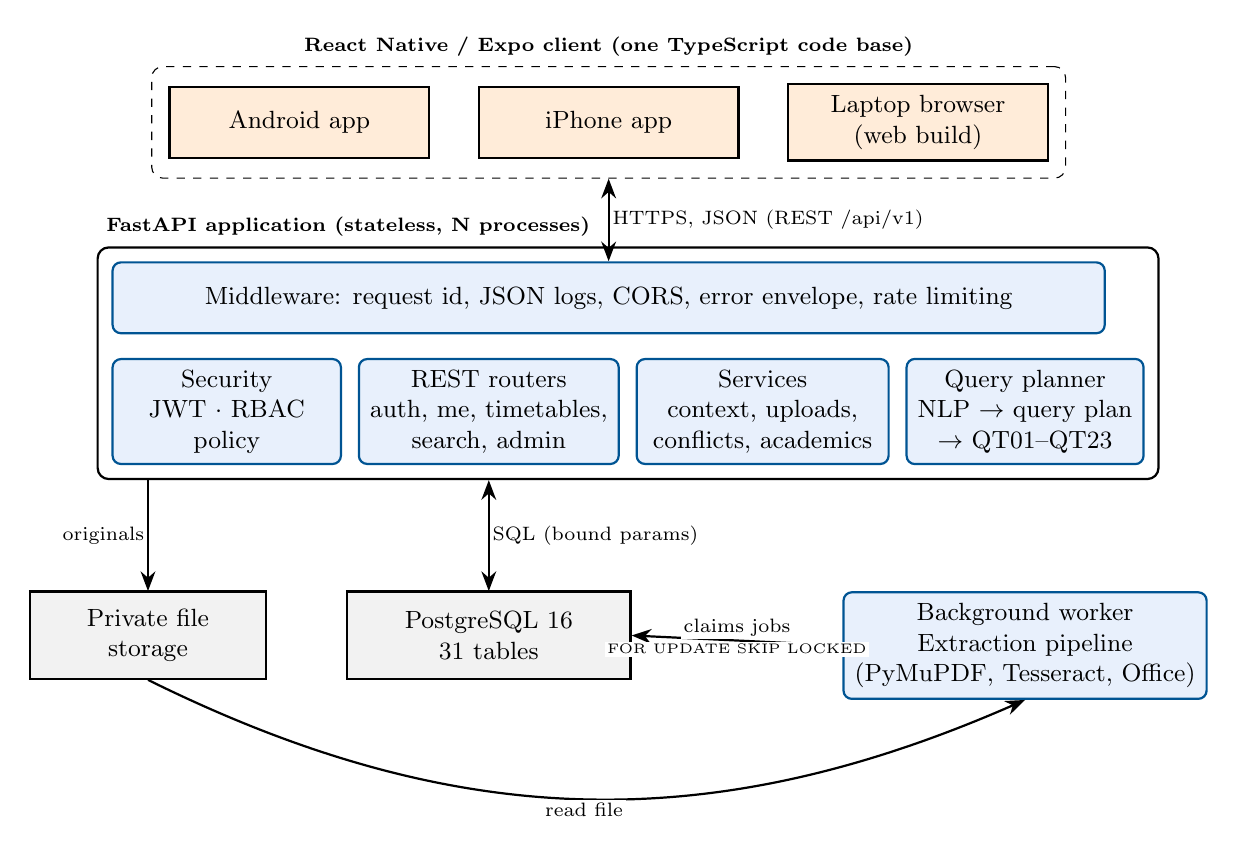
\begin{tikzpicture}[node distance=4mm and 6mm]
% clients
\node[ext,minimum width=3.3cm] (android) {Android app};
\node[ext,minimum width=3.3cm,right=of android] (ios) {iPhone app};
\node[ext,minimum width=3.3cm,right=of ios] (web) {Laptop browser\\(web build)};
\node[draw,dashed,rounded corners,fit=(android)(ios)(web),inner sep=6pt,
      label={[font=\scriptsize\bfseries]above:React Native / Expo client (one TypeScript code base)}] (cl) {};
% api
\node[blk,below=13mm of ios,minimum width=12.6cm,minimum height=9mm] (mw) {Middleware: request id, JSON logs, CORS, error envelope, rate limiting};
\node[blk,below=3mm of mw.south west,anchor=north west,minimum width=2.9cm,minimum height=13mm] (sec) {Security\\JWT $\cdot$ RBAC\\policy};
\node[blk,right=2mm of sec,minimum width=2.9cm,minimum height=13mm] (routers) {REST routers\\auth, me, timetables,\\search, admin};
\node[blk,right=2mm of routers,minimum width=3.2cm,minimum height=13mm] (svc) {Services\\context, uploads,\\conflicts, academics};
\node[blk,right=2mm of svc,minimum width=3cm,minimum height=13mm] (qe) {Query planner\\NLP $\rightarrow$ query plan\\$\rightarrow$ QT01--QT23};
\node[draw,thick,rounded corners,fit=(mw)(sec)(qe),inner sep=5pt,
      label={[font=\scriptsize\bfseries,anchor=south west]north west:FastAPI application (stateless, N processes)}] (api) {};
% bottom
\node[store,below=16mm of routers,minimum width=3.6cm,minimum height=11mm,font=\small] (db) {PostgreSQL 16\\31 tables};
\node[blk,below=16mm of qe,minimum width=4cm,minimum height=11mm] (worker) {Background worker\\Extraction pipeline\\(PyMuPDF, Tesseract, Office)};
\node[store,left=10mm of db,minimum width=3cm,minimum height=11mm,font=\small] (files) {Private file\\storage};
\draw[darr] (cl.south) -- node[lbl,right]{HTTPS, JSON (REST /api/v1)} (mw.north -| cl.south);
\draw[darr] (api.south -| db.north) -- node[lbl,right]{SQL (bound params)} (db.north);
\draw[arr] (worker.west) -- node[lbl,above]{claims jobs} node[lbl,below,font=\tiny]{FOR UPDATE SKIP LOCKED} (db.east);
\draw[arr] (api.south -| files.north) -- node[lbl,left]{originals} (files.north);
\draw[arr] (files.south) to[bend right=25] node[lbl,below]{read file} (worker.south);
\end{tikzpicture}
\caption{Overall system architecture (block diagram)}
\label{fig:arch}
\end{figure}

\paragraph{Responsibilities and interactions.}
The \textbf{client} renders dashboards and forms, caches reads with TanStack Query and keeps the
session in the device keystore. It calls the \textbf{API} over HTTPS with a bearer token. The API
authenticates the user, loads roles from the database, resolves the search context (domain,
timetable, time zone, current time), and runs services and the query engine. Uploads are stored
privately and a \texttt{PROCESSING\_JOB} row is inserted in the same transaction. The \textbf{worker}
claims jobs, extracts and validates the timetable, and writes entries back. \textbf{PostgreSQL} is
the single source of truth, and its row locks are also used for synchronisation.

\subsection{Component and Module Description}
\begingroup\small
\begin{longtable}{@{}>{\raggedright\arraybackslash}p{3.3cm}>{\raggedright\arraybackslash}p{4.4cm}>{\raggedright\arraybackslash}p{3.5cm}>{\raggedright\arraybackslash}p{3.9cm}@{}}
\caption{Modules: purpose, inputs, outputs and dependencies}\label{tab:modules}\\
\toprule
\textbf{Module (path)} & \textbf{Purpose} & \textbf{Input / output} & \textbf{Depends on}\\
\midrule
\endfirsthead
\toprule
\textbf{Module (path)} & \textbf{Purpose} & \textbf{Input / output} & \textbf{Depends on}\\
\midrule
\endhead
Auth \& RBAC \newline{\scriptsize\texttt{app/\allowbreak security}} & Login, tokens, password hashing, role$\rightarrow$scope policy, rate limit & Credentials / tokens; request / principal & \texttt{USER\_ACCOUNT}, \texttt{USER\_ROLE}, Argon2, PyJWT\\
API routers \newline{\scriptsize\texttt{app/\allowbreak api/\allowbreak v1}} & HTTP endpoints, request/response validation & JSON, multipart / JSON envelopes & Services, Pydantic\\
Context resolver \newline{\scriptsize\texttt{services/\allowbreak context.py}} & Chooses domain, timetable, time zone, ``now'' on the server & User + hints / context object & Preferences, settings\\
Upload service \newline{\scriptsize\texttt{services/\allowbreak uploads.py}} & Validates file, stores it, creates archive + job & File / timetable id (\textsc{Queued}) & File types, storage, jobs\\
Extraction \newline{\scriptsize\texttt{app/\allowbreak extraction}} & File $\rightarrow$ grid $\rightarrow$ sections, times, cells $\rightarrow$ validated entries & Bytes / \texttt{ExtractionResult} & PyMuPDF, Tesseract, openpyxl, python-docx\\
Worker \newline{\scriptsize\texttt{app/\allowbreak worker.py}} & Claims and runs jobs, heartbeat, retries, status update & Job rows / entries, status, notification & Extraction, DB\\
Query planner \newline{\scriptsize\texttt{app/\allowbreak query}} & Parse, build a typed query plan, resolve entities, validate, compile into templates (specialised QT01--QT22 or composed QT23) & Text / result envelope & Vocabulary, templates, policy\\
Conflicts \newline{\scriptsize\texttt{services/\allowbreak conflicts.py}} & Detect professor/room/batch overlaps & Timetable id / conflict list & Entries\\
Academics \newline{\scriptsize\texttt{services/\allowbreak academics.py}} & Fresher registration, promotion, transitions & Admin commands / history rows & Student history\\
Admin master data & Departments, years, batches, courses, rooms, aliases, users & Forms / records & DB, audit\\
Notifications \& audit & In-app/push notifications; audit trail & Events / rows & Expo push (optional)\\
Mobile app \newline{\scriptsize\texttt{mobile/\allowbreak src}} & Screens, navigation, state, API client & User actions / rendered UI & REST API\\
\bottomrule
\end{longtable}
\endgroup

\subsection{Architecture Selection and Justification}
We compared three options.
\begin{enumerate}
\item \textbf{Microservices} (separate auth, extraction and search services with a message broker):
      independent scaling, but much more deployment and debugging effort for a single-college workload and
      a team of students, and not possible on a free hosting tier.
\item \textbf{Serverless functions}: no server to manage, but cold starts, execution-time limits
      that do not suit OCR, and vendor lock-in.
\item \textbf{Modular monolith + worker} (chosen): one Python service with clearly separated
      layers (API $\rightarrow$ services $\rightarrow$ query/extraction $\rightarrow$ data). The only
      CPU-heavy part, extraction, runs in a separate worker process so it never blocks API requests.
      A PostgreSQL job table replaces a message broker, so job creation is in the \emph{same
      transaction} as the upload record and there is one less moving part.
\end{enumerate}
The API is \textbf{stateless} (REST~\cite{fielding2000}): any process can serve any request, so the
system scales horizontally by adding processes. A \textbf{layered} design keeps the rules
(security, domain separation) in one place each, which makes them testable.

\subsection{Data Flow Diagrams}
\begin{figure}[H]
\centering
\begin{adjustbox}{max width=\textwidth}
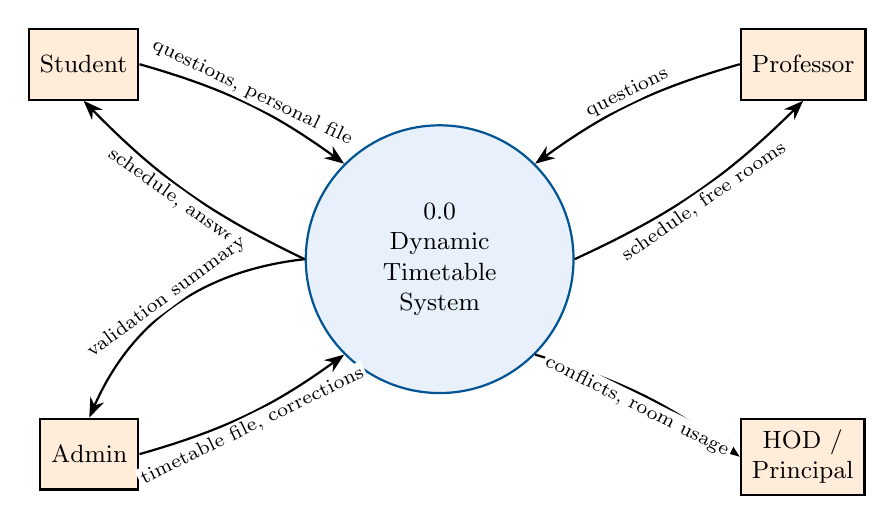
\begin{tikzpicture}
\node[proc,minimum size=34mm,font=\small] (sys) {0.0\\Dynamic\\Timetable\\System};
\node[ext,above left=8mm and 26mm of sys] (stu) {Student};
\node[ext,above right=8mm and 26mm of sys] (prof) {Professor};
\node[ext,below left=8mm and 26mm of sys] (adm) {Admin};
\node[ext,below right=8mm and 26mm of sys] (hod) {HOD /\\Principal};
\draw[arr] (stu.east) to[bend left=10] node[lbl,above,sloped]{questions, personal file} (sys.north west);
\draw[arr] (sys.west) to[bend left=10] node[lbl,below,sloped]{schedule, answers} (stu.south);
\draw[arr] (prof.west) to[bend right=10] node[lbl,above,sloped]{questions} (sys.north east);
\draw[arr] (sys.east) to[bend right=10] node[lbl,below,sloped]{schedule, free rooms} (prof.south);
\draw[arr] (adm.east) to[bend right=10] node[lbl,below,sloped]{timetable file, corrections} (sys.south west);
\draw[arr] (sys.west) to[bend right=30] node[lbl,above,sloped]{validation summary} (adm.north);
\draw[arr] (sys.south east) to[bend left=10] node[lbl,below,sloped]{conflicts, room usage} (hod.west);
\end{tikzpicture}
\end{adjustbox}
\caption{DFD level 0 (context diagram)}
\label{fig:dfd0}
\end{figure}

\begin{figure}[H]
\centering
\begin{adjustbox}{max width=\textwidth}
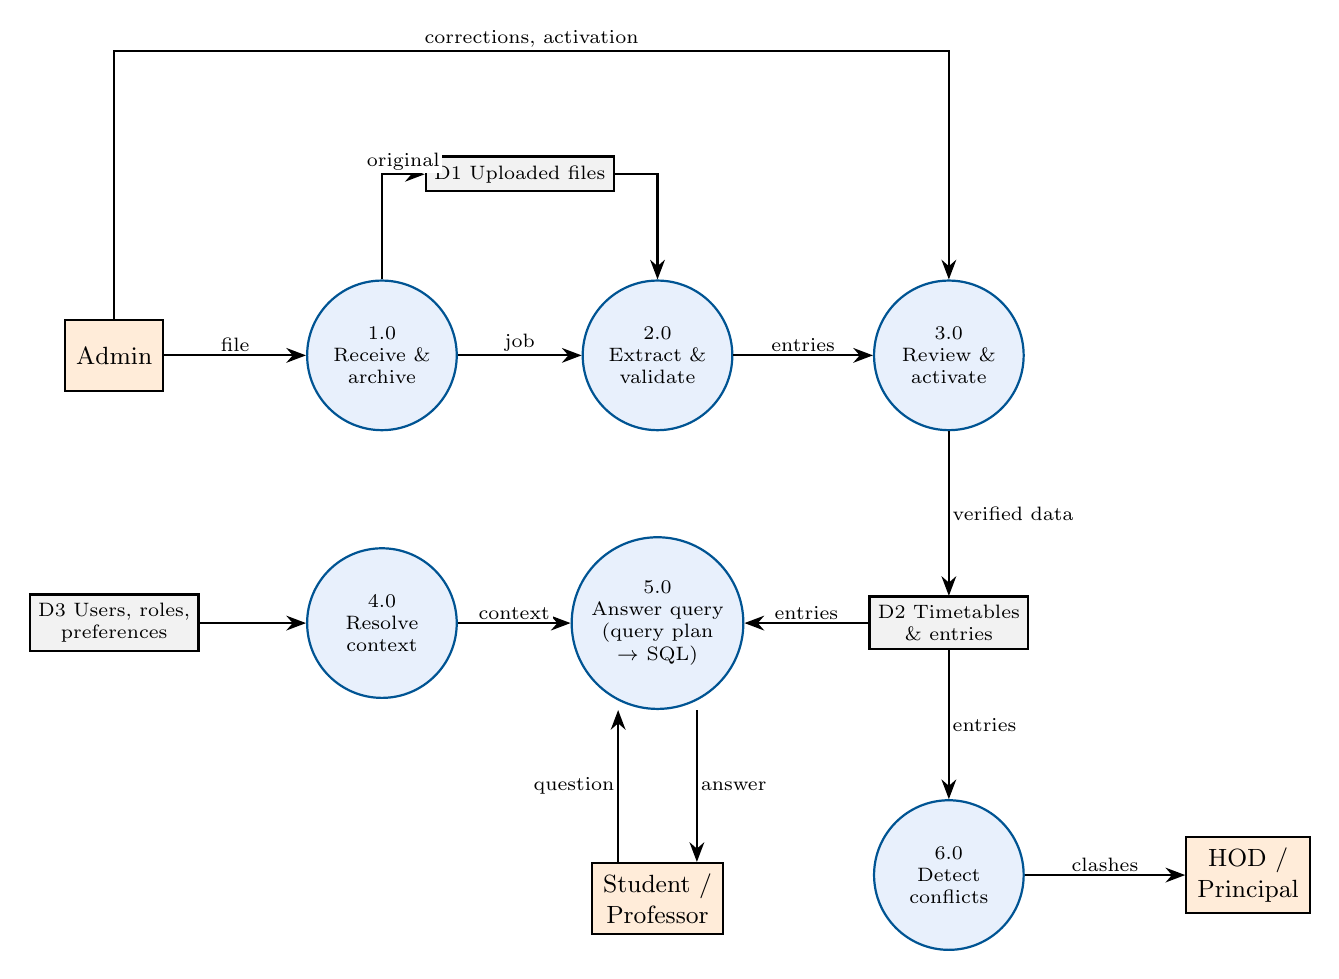
\begin{tikzpicture}
\node[ext] (adm) at (0,0) {Admin};
\node[proc] (p1) at (3.4,0) {1.0\\Receive \&\\archive};
\node[proc] (p2) at (6.9,0) {2.0\\Extract \&\\validate};
\node[proc] (p3) at (10.6,0) {3.0\\Review \&\\activate};
\node[store] (d1) at (5.15,2.3) {D1 Uploaded files};
\node[store] (d3) at (0,-3.4) {D3 Users, roles,\\preferences};
\node[proc] (p4) at (3.4,-3.4) {4.0\\Resolve\\context};
\node[proc] (p5) at (6.9,-3.4) {5.0\\Answer query\\(query plan\\$\rightarrow$ SQL)};
\node[store] (d2) at (10.6,-3.4) {D2 Timetables\\\& entries};
\node[proc] (p6) at (10.6,-6.6) {6.0\\Detect\\conflicts};
\node[ext] (hod) at (14.4,-6.6) {HOD /\\Principal};
\node[ext] (usr) at (6.9,-6.9) {Student /\\Professor};
\draw[arr] (adm) -- node[lbl,above]{file} (p1);
\draw[arr] (p1) -- node[lbl,above]{job} (p2);
\draw[arr] (p1) |- node[lbl,pos=0.75,above]{original} (d1.west);
\draw[arr] (d1.east) -| (p2);
\draw[arr] (p2) -- node[lbl,above]{entries} (p3);
\draw[arr] (adm.north) -- ++(0,3.4) -| node[lbl,pos=0.25,above]{corrections, activation} (p3.north);
\draw[arr] (p3) -- node[lbl,right]{verified data} (d2);
\draw[arr] (d3) -- (p4);
\draw[arr] (p4) -- node[lbl,above]{context} (p5);
\draw[arr] (d2) -- node[lbl,above]{entries} (p5);
\draw[arr] (d2) -- node[lbl,right]{entries} (p6);
\draw[arr] (p6) -- node[lbl,above]{clashes} (hod);
\draw[arr] ([xshift=-5mm]usr.north) -- node[lbl,left]{question} ([xshift=-5mm]p5.south);
\draw[arr] ([xshift=5mm]p5.south) -- node[lbl,right]{answer} ([xshift=5mm]usr.north);
\end{tikzpicture}
\end{adjustbox}
\caption{DFD level 1}
\label{fig:dfd1}
\end{figure}
The level-0 DFD shows the system with its four external entities. The level-1 DFD splits it into the
upload path (1.0--3.0, used by the Admin) and the query path (4.0--6.0, used by everyone). Both
share the timetable store D2. Personal timetables follow the same path but are written to separate
personal tables (not drawn).

\subsection{UML Diagrams}
\subsubsection{Use case diagram}
\begin{figure}[H]
\centering
\begin{adjustbox}{max width=\textwidth}
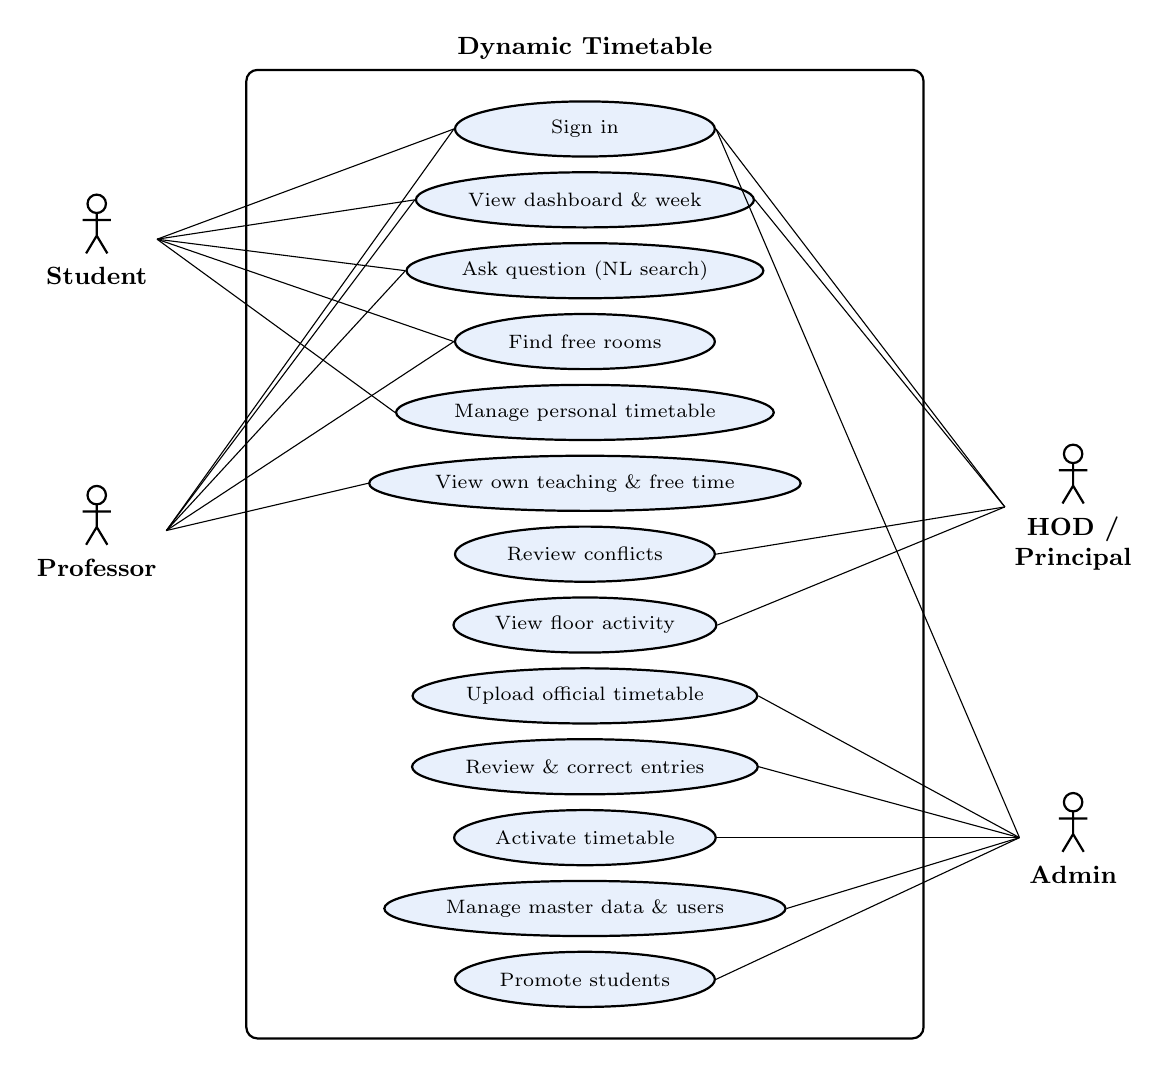
\begin{tikzpicture}[uc/.style={draw,ellipse,thick,fill=boxfill,font=\scriptsize,align=center,minimum width=33mm,minimum height=7mm,inner sep=1pt},
  actor/.style={font=\small,align=center}]
\node[draw,thick,rounded corners,minimum width=8.6cm,minimum height=12.3cm,label={[font=\small\bfseries]above:Dynamic Timetable}] (b) at (0,0) {};
\foreach \n/\t/\y in {u1/Sign in/5.4, u2/View dashboard \& week/4.5, u3/Ask question (NL search)/3.6, u4/Find free rooms/2.7,
  u5/Manage personal timetable/1.8, u6/View own teaching \& free time/0.9, u7/Review conflicts/0, u8/View floor activity/-0.9,
  u9/Upload official timetable/-1.8, u10/Review \& correct entries/-2.7, u11/Activate timetable/-3.6, u12/Manage master data \& users/-4.5, u13/Promote students/-5.4}
  { \node[uc] (\n) at (0,\y) {\t}; }
\node[actor] (s) at (-6.2,4) {\stick\\\textbf{Student}};
\node[actor] (p) at (-6.2,0.3) {\stick\\\textbf{Professor}};
\node[actor] (h) at (6.2,0.6) {\stick\\\textbf{HOD /}\\\textbf{Principal}};
\node[actor] (a) at (6.2,-3.6) {\stick\\\textbf{Admin}};
\foreach \u in {u1,u2,u3,u4,u5} \draw (s.east) -- (\u.west);
\foreach \u in {u1,u2,u3,u4,u6} \draw (p.east) -- (\u.west);
\foreach \u in {u1,u2,u7,u8} \draw (h.west) -- (\u.east);
\foreach \u in {u1,u9,u10,u11,u12,u13} \draw (a.west) -- (\u.east);
\end{tikzpicture}
\end{adjustbox}
\caption{Use case diagram}
\label{fig:usecase}
\end{figure}
Professors inherit the student-facing use cases. The HOD and Principal are professors with wider scopes,
which is why the system uses many-to-many \texttt{USER\_ROLE} rather than one role per user.

\subsubsection{Class diagram}
\begin{figure}[H]
\centering
\resizebox{\textwidth}{!}{%
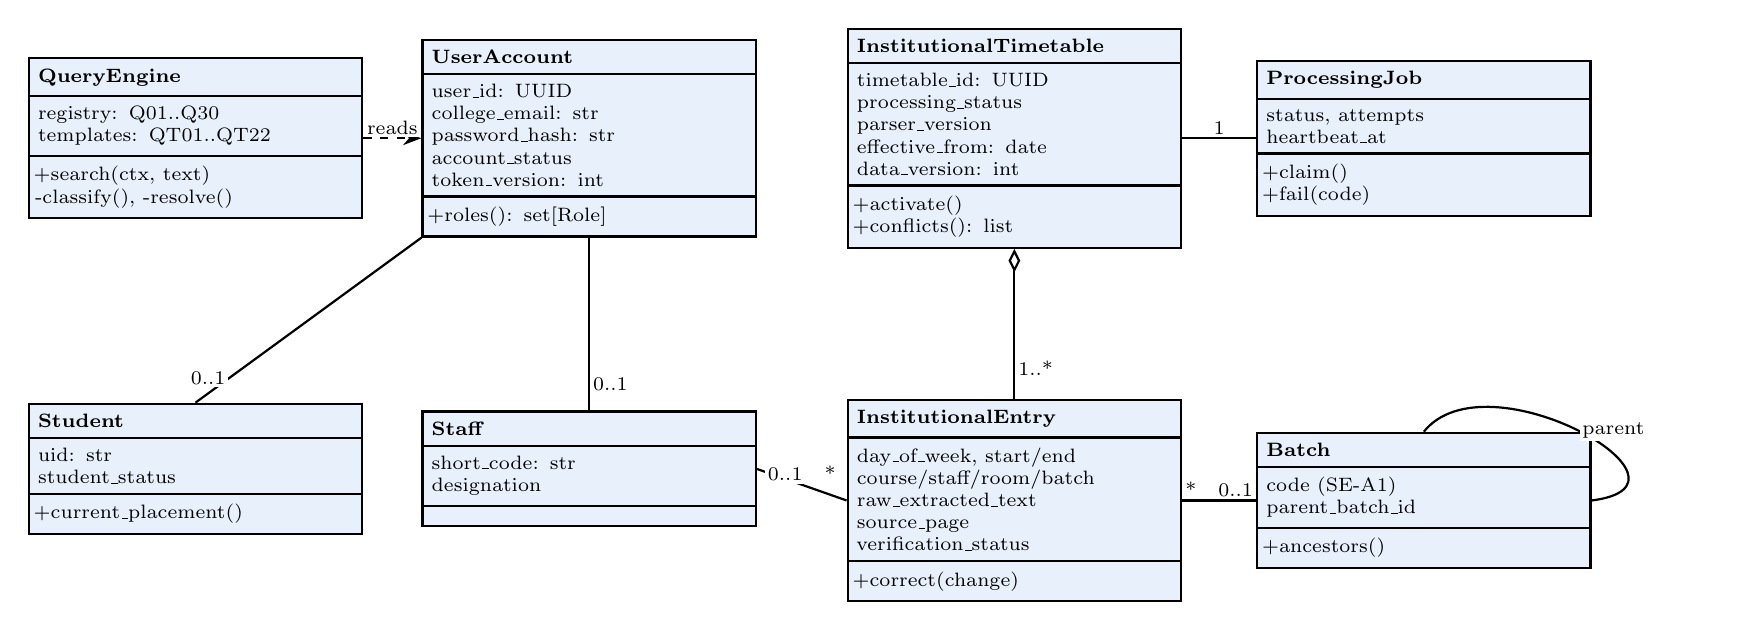
\begin{tikzpicture}[cls/.style={draw,thick,rectangle split,rectangle split parts=3,fill=boxfill,
  font=\scriptsize,align=left,text width=40mm,rectangle split part fill={spitblue!25,boxfill,white}}]
\node[cls] (ua) at (0,0) {\textbf{UserAccount}
\nodepart{second}user\_id: UUID\\college\_email: str\\password\_hash: str\\account\_status\\token\_version: int
\nodepart{third}+roles(): set[Role]};
\node[cls] (st) at (-5,-4.2) {\textbf{Student}
\nodepart{second}uid: str\\student\_status
\nodepart{third}+current\_placement()};
\node[cls] (sf) at (0,-4.2) {\textbf{Staff}
\nodepart{second}short\_code: str\\designation
\nodepart{third}};
\node[cls] (it) at (5.4,0) {\textbf{InstitutionalTimetable}
\nodepart{second}timetable\_id: UUID\\processing\_status\\parser\_version\\effective\_from: date\\data\_version: int
\nodepart{third}+activate()\\+conflicts(): list};
\node[cls] (ie) at (5.4,-4.6) {\textbf{InstitutionalEntry}
\nodepart{second}day\_of\_week, start/end\\course/staff/room/batch\\raw\_extracted\_text\\source\_page\\verification\_status
\nodepart{third}+correct(change)};
\node[cls] (job) at (10.6,0) {\textbf{ProcessingJob}
\nodepart{second}status, attempts\\heartbeat\_at
\nodepart{third}+claim()\\+fail(code)};
\node[cls] (qe) at (-5,0) {\textbf{QueryEngine}
\nodepart{second}registry: Q01..Q30\\templates: QT01..QT22
\nodepart{third}+search(ctx, text)\\-classify(), -resolve()};
\node[cls] (b) at (10.6,-4.6) {\textbf{Batch}
\nodepart{second}code (SE-A1)\\parent\_batch\_id
\nodepart{third}+ancestors()};
\draw[thick] (ua.south) -- node[lbl,pos=.85,right]{0..1} (sf.north);
\draw[thick] (ua.south west) -- node[lbl,pos=.85,left]{0..1} (st.north);
\draw[thick,-{Diamond[open,length=3mm]}] (ie.north) -- node[lbl,pos=0.2,right]{1..*} (it.south);
\draw[thick] (job.west) -- node[lbl,above]{1} (it.east);
\draw[thick,dashed,-{Stealth}] (qe.east) -- node[lbl,above]{reads} (ua.west);
\draw[thick] (ie.east) -- node[lbl,above]{*\quad 0..1} (b.west);
\draw[thick] (sf.east) -- node[lbl,above]{0..1\quad *} (ie.west);
\draw[thick] (b.north) .. controls +(0.8,1) and +(1.6,0.2) .. node[lbl,right]{parent} (b.east);
\end{tikzpicture}}
\caption{Simplified class diagram of the core domain}
\label{fig:class}
\end{figure}

\subsubsection{Sequence diagram: answering a question}
\begin{figure}[H]
\centering
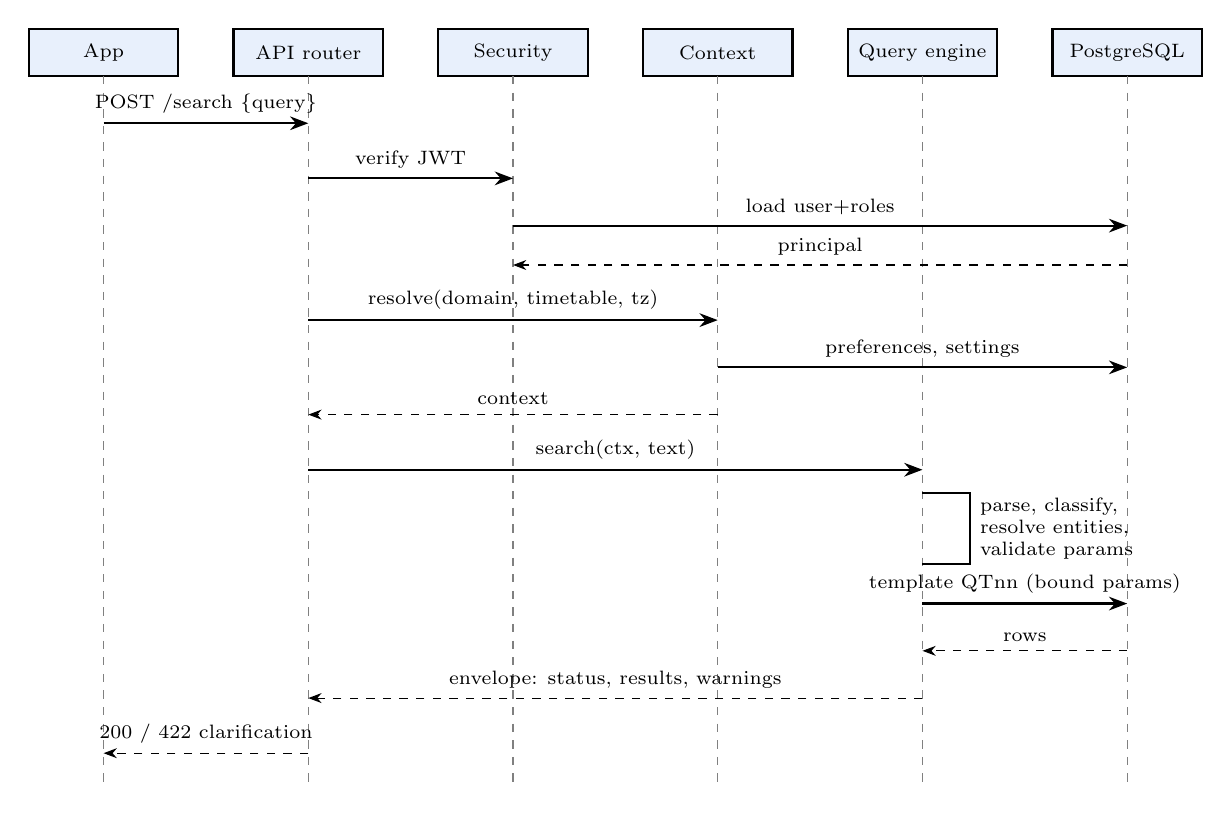
\begin{tikzpicture}[
  ll/.style={draw,thick,fill=boxfill,font=\scriptsize,minimum width=19mm,minimum height=6mm},
  msg/.style={-{Stealth},thick,font=\scriptsize},
  ret/.style={-{Stealth},dashed,font=\scriptsize}]
\foreach \x/\n/\t in {0/c/App, 2.6/a/API router, 5.2/s/Security, 7.8/x/Context, 10.4/q/Query engine, 13.0/d/PostgreSQL}{
  \node[ll] (\n) at (\x,0) {\t};
  \draw[dashed,gray] (\x,-0.3) -- (\x,-9.3);}
\draw[msg] (0,-0.9) -- node[above]{POST /search \{query\}} (2.6,-0.9);
\draw[msg] (2.6,-1.6) -- node[above]{verify JWT} (5.2,-1.6);
\draw[msg] (5.2,-2.2) -- node[above]{load user+roles} (13,-2.2);
\draw[ret] (13,-2.7) -- node[above]{principal} (5.2,-2.7);
\draw[msg] (2.6,-3.4) -- node[above]{resolve(domain, timetable, tz)} (7.8,-3.4);
\draw[msg] (7.8,-4.0) -- node[above]{preferences, settings} (13,-4.0);
\draw[ret] (7.8,-4.6) -- node[above]{context} (2.6,-4.6);
\draw[msg] (2.6,-5.3) -- node[above]{search(ctx, text)} (10.4,-5.3);
\draw[thick] (10.4,-5.6) -- ++(0.6,0) -- node[right,font=\scriptsize,align=left]{parse, classify,\\resolve entities,\\validate params} ++(0,-0.9) -- ++(-0.6,0);
\draw[msg] (10.4,-7.0) -- node[above]{template QTnn (bound params)} (13,-7.0);
\draw[ret] (13,-7.6) -- node[above]{rows} (10.4,-7.6);
\draw[ret] (10.4,-8.2) -- node[above]{envelope: status, results, warnings} (2.6,-8.2);
\draw[ret] (2.6,-8.9) -- node[above]{200 / 422 clarification} (0,-8.9);
\end{tikzpicture}
\caption{Sequence diagram for a natural-language search}
\label{fig:seq}
\end{figure}
Identity, roles and the selected timetable are always resolved on the server, so the client cannot
claim another role or timetable. If a parameter is missing (for example a.m./p.m.), the engine
returns \texttt{CLARIFICATION\_REQUIRED} with choices instead of running a template.

\subsubsection{Activity diagram: publishing a new timetable}
\begin{figure}[H]
\centering
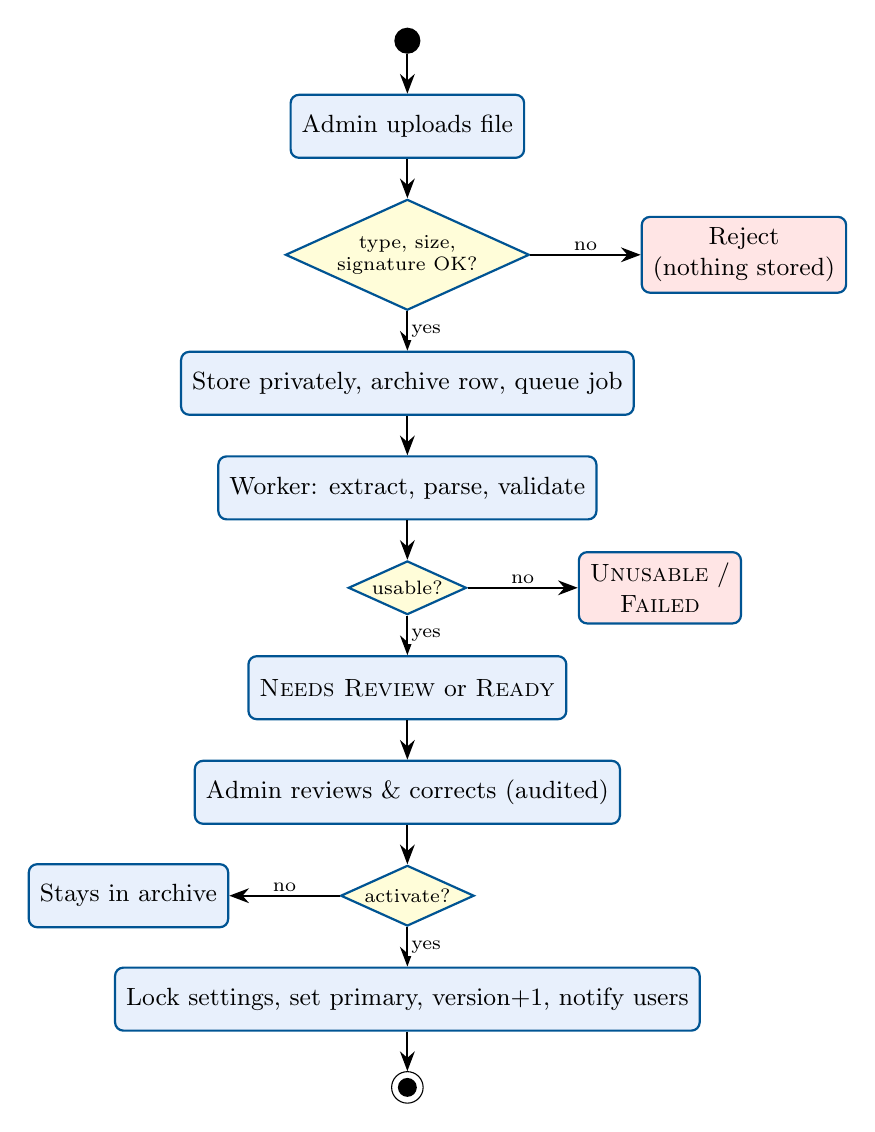
\begin{tikzpicture}[node distance=5mm]
\node[fill=black,circle,minimum size=3mm] (s) {};
\node[blk,below=of s] (a1) {Admin uploads file};
\node[dec,below=of a1] (d1) {type, size,\\signature OK?};
\node[blk,right=14mm of d1,fill=red!10] (rej) {Reject\\(nothing stored)};
\node[blk,below=of d1] (a2) {Store privately, archive row, queue job};
\node[blk,below=of a2] (a3) {Worker: extract, parse, validate};
\node[dec,below=of a3] (d2) {usable?};
\node[blk,right=14mm of d2,fill=red!10] (un) {\textsc{Unusable} /\\\textsc{Failed}};
\node[blk,below=of d2] (a4) {\textsc{Needs Review} or \textsc{Ready}};
\node[blk,below=of a4] (a5) {Admin reviews \& corrects (audited)};
\node[dec,below=of a5] (d3) {activate?};
\node[blk,below=of d3] (a6) {Lock settings, set primary, version+1, notify users};
\node[draw,circle,minimum size=4mm,below=of a6,path picture={\fill (path picture bounding box.center) circle (1.2mm);}] (e) {};
\node[blk,left=14mm of d3] (keep) {Stays in archive};
\draw[arr] (s) -- (a1); \draw[arr] (a1) -- (d1); \draw[arr] (d1) -- node[lbl,above]{no} (rej);
\draw[arr] (d1) -- node[lbl,right]{yes} (a2); \draw[arr] (a2) -- (a3); \draw[arr] (a3) -- (d2);
\draw[arr] (d2) -- node[lbl,above]{no} (un); \draw[arr] (d2) -- node[lbl,right]{yes} (a4);
\draw[arr] (a4) -- (a5); \draw[arr] (a5) -- (d3); \draw[arr] (d3) -- node[lbl,right]{yes} (a6); \draw[arr] (a6) -- (e);
\draw[arr] (d3) -- node[lbl,above]{no} (keep);
\end{tikzpicture}
\caption{Activity diagram: upload, review and activation}
\label{fig:activity}
\end{figure}

\subsubsection{State machine diagram: timetable processing status}
\begin{figure}[H]
\centering
\begin{adjustbox}{max width=\textwidth}
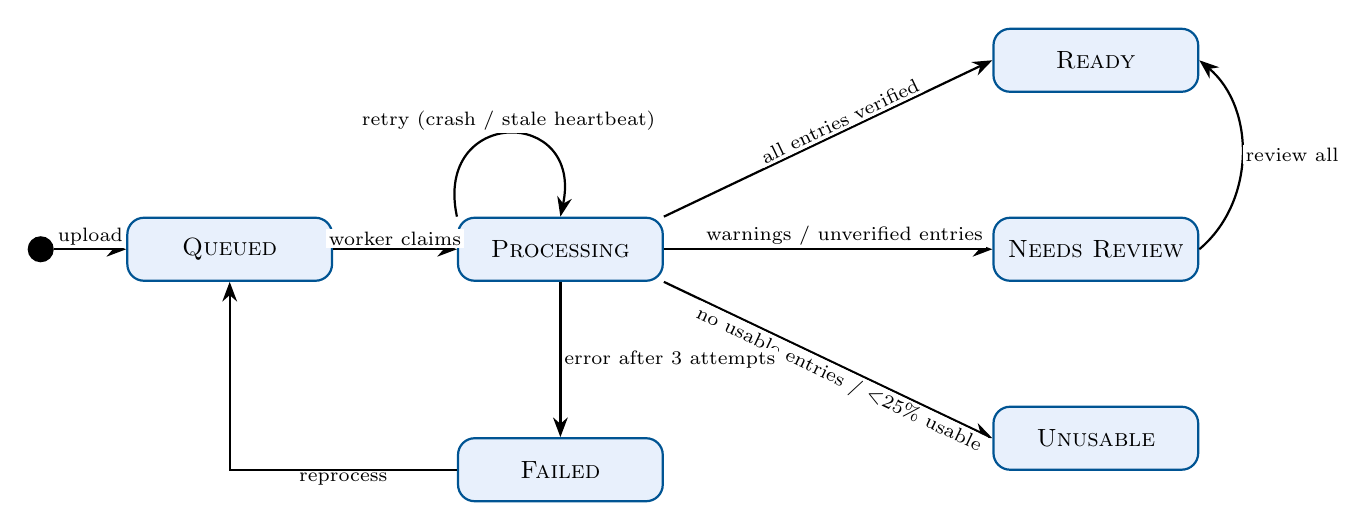
\begin{tikzpicture}[st/.style={draw=spitblue,thick,rounded corners=6pt,fill=boxfill,font=\small,minimum width=26mm,minimum height=8mm}]
\node[fill=black,circle,minimum size=3mm] (i) at (-2.4,0) {};
\node[st] (q) at (0,0) {\textsc{Queued}};
\node[st] (p) at (4.2,0) {\textsc{Processing}};
\node[st] (r) at (11,2.4) {\textsc{Ready}};
\node[st] (n) at (11,0) {\textsc{Needs Review}};
\node[st] (u) at (11,-2.4) {\textsc{Unusable}};
\node[st] (f) at (4.2,-2.8) {\textsc{Failed}};
\draw[arr] (i) -- node[lbl,above]{upload} (q);
\draw[arr] (q) -- node[lbl,above]{worker claims} (p);
\draw[arr] (p.north east) -- node[lbl,above,sloped,pos=0.55]{all entries verified} (r.west);
\draw[arr] (p) -- node[lbl,above,pos=0.55]{warnings / unverified entries} (n);
\draw[arr] (p.south east) -- node[lbl,below,sloped,pos=0.55]{no usable entries / $<$25\% usable} (u.west);
\draw[arr] (p) -- node[lbl,right]{error after 3 attempts} (f);
\draw[arr] (p.north west) .. controls +(-0.3,1.4) and +(0.3,1.4) .. node[lbl,above]{retry (crash / stale heartbeat)} (p.north);
\draw[arr] (n.east) to[bend right=50] node[lbl,right]{review all} (r.east);
\draw[arr] (f.west) -| node[lbl,pos=0.25,below]{reprocess} (q.south);
\end{tikzpicture}
\end{adjustbox}
\caption{State machine of a timetable archive (\textsc{Ready} and \textsc{Needs Review} may be activated)}
\label{fig:state}
\end{figure}

\subsubsection{Deployment diagram}
\begin{figure}[H]
\centering
\begin{adjustbox}{max width=\textwidth}
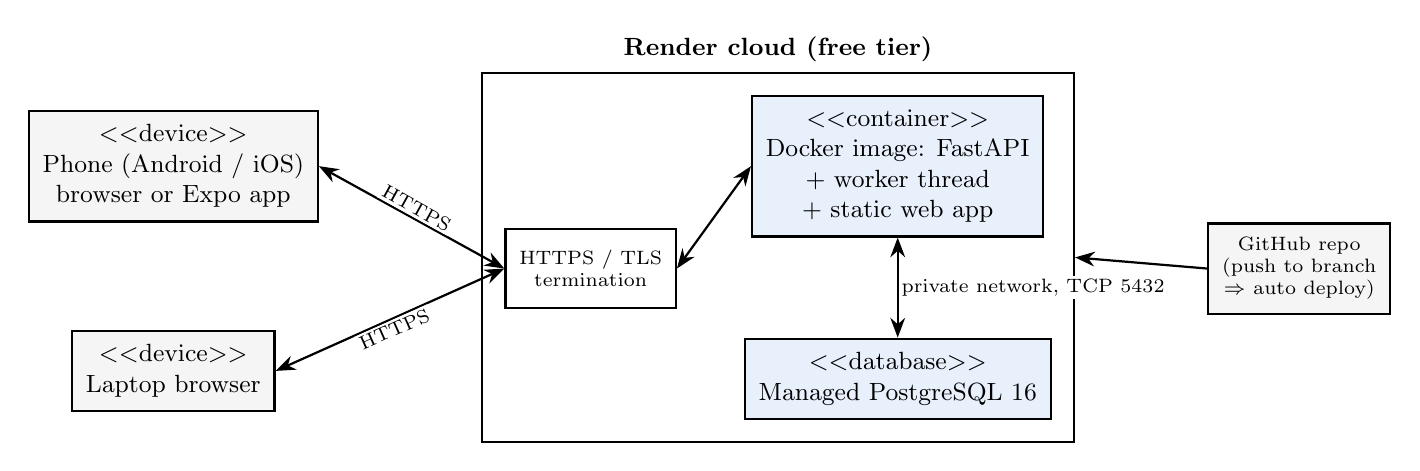
\begin{tikzpicture}[node/.style={draw,thick,fill=gray!8,align=center,font=\small,minimum height=10mm,inner sep=5pt}]
\node[node] (ph) at (0,0) {\textless\textless device\textgreater\textgreater\\Phone (Android / iOS)\\browser or Expo app};
\node[node] (lp) at (0,-2.6) {\textless\textless device\textgreater\textgreater\\Laptop browser};
\node[node,fill=white,font=\scriptsize] (tls) at (5.3,-1.3) {HTTPS / TLS\\termination};
\node[node,fill=boxfill] (svc) at (9.2,0) {\textless\textless container\textgreater\textgreater\\Docker image: FastAPI\\+ worker thread\\+ static web app};
\node[node,fill=boxfill] (pg) at (9.2,-2.7) {\textless\textless database\textgreater\textgreater\\Managed PostgreSQL 16};
\node[draw,thick,fit=(tls)(svc)(pg),inner sep=8pt,label={[font=\small\bfseries]above:Render cloud (free tier)}] (cloud) {};
\node[node,font=\scriptsize] (gh) at (14.3,-1.3) {GitHub repo\\(push to branch\\$\Rightarrow$ auto deploy)};
\draw[darr] (ph.east) -- node[lbl,above,sloped]{HTTPS} (tls.west);
\draw[darr] (lp.east) -- node[lbl,below,sloped]{HTTPS} (tls.west);
\draw[darr] (tls.east) -- (svc.west);
\draw[darr] (svc) -- node[lbl,right]{private network, TCP 5432} (pg);
\draw[arr] (gh.west) -- (cloud.east);
\end{tikzpicture}
\end{adjustbox}
\caption{Deployment diagram of the free online demo}
\label{fig:deploy}
\end{figure}
For the demo, the worker runs as a thread inside the web container, because the free tier allows one
service. In production the API and the worker run as separate processes or containers
(\texttt{docker-compose.yml}).

\subsection{Database Design}
\subsubsection{ER diagram}
\begin{figure}[H]
\centering
\begin{adjustbox}{max width=\textwidth}
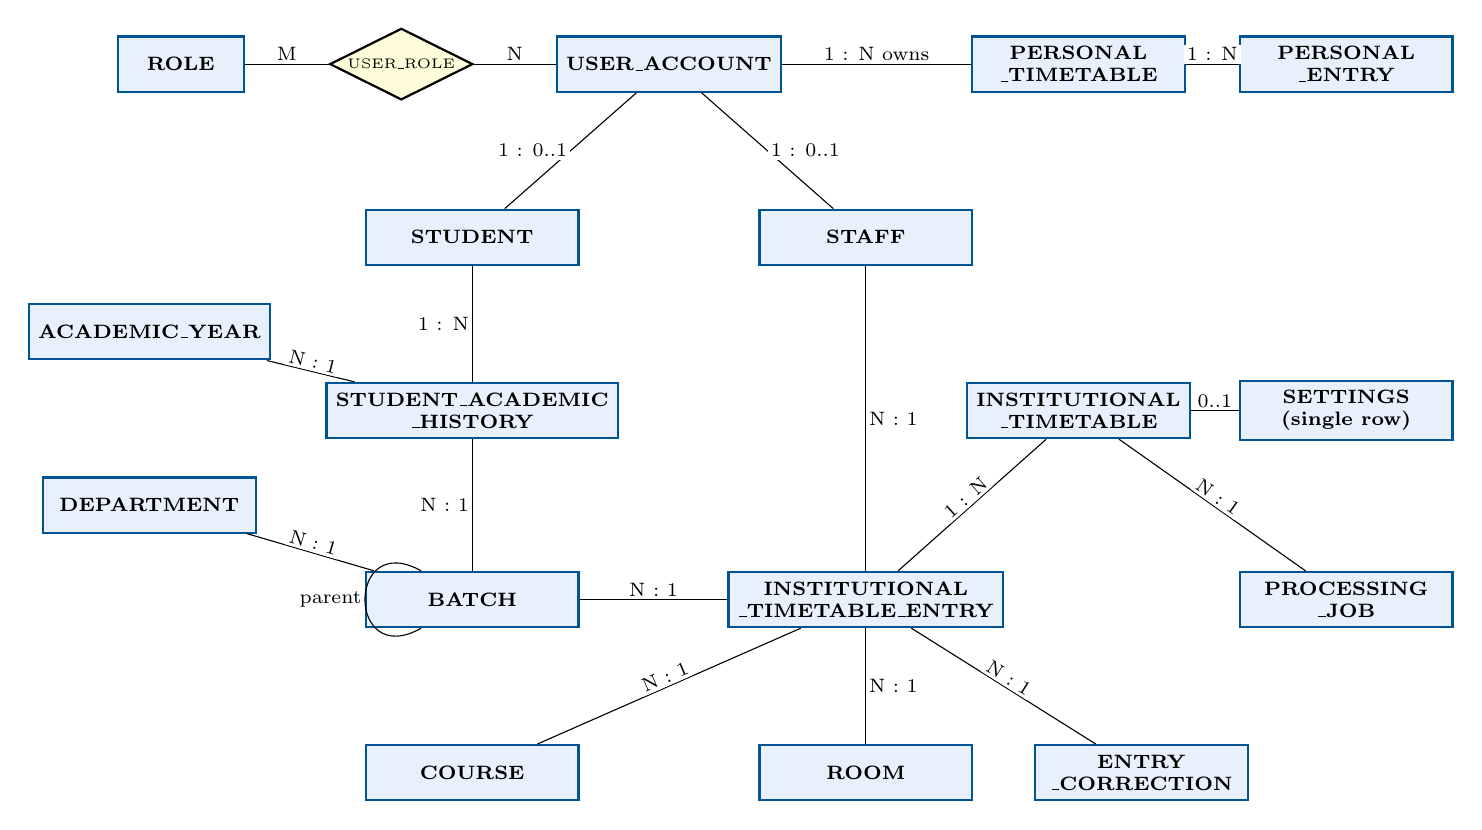
\begin{tikzpicture}[ent/.style={draw=spitblue,thick,fill=boxfill,font=\scriptsize\bfseries,minimum width=27mm,minimum height=7mm,align=center},
  rel/.style={draw,thick,diamond,aspect=2,fill=yellow!15,font=\tiny,inner sep=1pt,align=center}]
\node[ent] (ua) at (0,0) {USER\_ACCOUNT};
\node[ent,minimum width=16mm] (role) at (-6.2,0) {ROLE};
\node[rel] (has) at (-3.4,0) {USER\_ROLE};
\node[ent] (stu) at (-2.5,-2.2) {STUDENT};
\node[ent] (stf) at (2.5,-2.2) {STAFF};
\node[ent] (sah) at (-2.5,-4.4) {STUDENT\_ACADEMIC\\\_HISTORY};
\node[ent] (batch) at (-2.5,-6.8) {BATCH};
\node[ent] (dept) at (-6.6,-5.6) {DEPARTMENT};
\node[ent] (ay) at (-6.6,-3.4) {ACADEMIC\_YEAR};
\node[ent] (itt) at (5.2,-4.4) {INSTITUTIONAL\\\_TIMETABLE};
\node[ent] (ite) at (2.5,-6.8) {INSTITUTIONAL\\\_TIMETABLE\_ENTRY};
\node[ent] (room) at (2.5,-9) {ROOM};
\node[ent] (course) at (-2.5,-9) {COURSE};
\node[ent] (set) at (8.6,-4.4) {SETTINGS\\(single row)};
\node[ent] (ptt) at (5.2,0) {PERSONAL\\\_TIMETABLE};
\node[ent] (pte) at (8.6,0) {PERSONAL\\\_ENTRY};
\node[ent] (job) at (8.6,-6.8) {PROCESSING\\\_JOB};
\node[ent] (cor) at (6,-9) {ENTRY\\\_CORRECTION};
\draw (role) -- node[lbl,above]{M} (has) -- node[lbl,above]{N} (ua);
\draw (ua) -- node[lbl,left]{1 : 0..1} (stu);
\draw (ua) -- node[lbl,right]{1 : 0..1} (stf);
\draw (stu) -- node[lbl,left]{1 : N} (sah);
\draw (sah) -- node[lbl,left]{N : 1} (batch);
\draw (sah) -- node[lbl,above,sloped]{N : 1} (ay);
\draw (batch) -- node[lbl,above,sloped]{N : 1} (dept);
\draw (batch) .. controls +(-1.6,-0.9) and +(-1.6,0.9) .. node[lbl,left]{parent} (batch);
\draw (itt) -- node[lbl,above,sloped]{1 : N} (ite);
\draw (ite) -- node[lbl,above]{N : 1} (batch);
\draw (ite) -- node[lbl,right]{N : 1} (room);
\draw (ite) -- node[lbl,above,sloped]{N : 1} (course);
\draw (ite) -- node[lbl,right]{N : 1} (stf);
\draw (set) -- node[lbl,above]{0..1} (itt);
\draw (ua) -- node[lbl,above]{1 : N owns} (ptt);
\draw (ptt) -- node[lbl,above]{1 : N} (pte);
\draw (job) -- node[lbl,above,sloped]{N : 1} (itt);
\draw (cor) -- node[lbl,above,sloped]{N : 1} (ite);
\end{tikzpicture}
\end{adjustbox}
\caption{ER diagram (main entities; personal sections, notifications, tokens and audit omitted)}
\label{fig:er}
\end{figure}

\subsubsection{Relational schema, keys and constraints}
The database has 31 tables, created by three Alembic migrations. Table~\ref{tab:schema} lists the most
important tables. Primary keys are UUIDs for user-facing objects (non-guessable, which prevents ID
enumeration) and \texttt{BIGINT} identities for master data.

\begingroup\footnotesize
\begin{longtable}{@{}>{\raggedright\arraybackslash}p{4.0cm}>{\raggedright\arraybackslash}p{5.6cm}>{\raggedright\arraybackslash}p{5.6cm}@{}}
\caption{Relational schema of the main tables}\label{tab:schema}\\
\toprule
\textbf{Table (PK)} & \textbf{Main attributes} & \textbf{FKs and constraints}\\
\midrule
\endfirsthead
\toprule
\textbf{Table (PK)} & \textbf{Main attributes} & \textbf{FKs and constraints}\\
\midrule
\endhead
\texttt{user\_\allowbreak{}account}\newline(user\_id) & college\_email, display\_name, password\_hash, account\_status, token\_version & UNIQUE(college\_email)\\
\texttt{user\_\allowbreak{}role}\newline(user\_id, role\_id) & -- & FK user, FK role (M:N bridge)\\
\texttt{student}\newline(student\_id) & uid, student\_status & FK user (UNIQUE), UNIQUE(uid)\\
\texttt{staff}\newline(staff\_id) & short\_code, designation & FK user (UNIQUE), FK department\\
\texttt{student\_\allowbreak{}academic\_\allowbreak{}history}\newline(history\_id) & year\_of\_study, semester, status, effective\_from/to & FK student, academic\_year, department, batch; \textbf{partial UNIQUE(student\_id) WHERE effective\_to IS NULL}\\
\texttt{batch}\newline(batch\_id) & code (SE-A1), cohort, division, program\_year & FK department, self-FK parent\_batch\_id; UNIQUE(dept, code)\\
\texttt{institutional\_\allowbreak{}timetable}\newline(timetable\_id) & title, file\_sha256, file\_format, processing\_status, parser\_version, effective\_from, data\_version & FK academic\_year, department, uploader; partial UNIQUE(uploader, client\_request\_id)\\
\texttt{institutional\_\allowbreak{}timetable\_\allowbreak{}entry}\newline(entry\_id) & entry\_kind, day\_of\_week, class\_date, start\_time, end\_time, raw labels, raw\_extracted\_text, source\_page, confidence\_score, verification\_status, time\_uncertain & FK timetable, section, course, batch, staff, room; CHECK day 1--7; CHECK end$>$start; CHECK status $\in$ \{VERIFIED, UNVERIFIED, INCOMPLETE, REJECTED\}; CHECK 0$\le$confidence$\le$1\\
\texttt{institutional\_\allowbreak{}timetable\_\allowbreak{}settings}\newline(settings\_id) & default\_timetable\_id, version, updated\_by & \textbf{CHECK settings\_id = 1} (single row)\\
\texttt{personal\_\allowbreak{}timetable}\newline(timetable\_id) & owner\_user\_id, status, \ldots & UNIQUE(timetable\_id, owner\_user\_id) for composite FKs\\
\texttt{user\_\allowbreak{}preference}\newline(user\_id) & selection\_mode, personal\_primary\_timetable\_id, last\_active\_domain, last institutional/personal timetable & \textbf{composite FKs (timetable\_id, owner\_user\_id)}: a user can only point to their own personal timetable\\
\texttt{processing\_\allowbreak{}job}\newline(job\_id) & domain, status, attempts, heartbeat\_at & CHECK exactly one target matching the domain\\
\texttt{entry\_\allowbreak{}correction}\newline(correction\_id) & domain, before/after JSON, reason, corrected\_by, corrected\_at & FK entry\\
\texttt{audit\_\allowbreak{}event}\newline(event\_id) & actor, event\_type, target\_type/id, request\_id, occurred\_at & append-only\\
\bottomrule
\end{longtable}
\endgroup

\paragraph{Normalisation.}
The schema is in third normal form: course, staff, room and batch details are stored once and
referenced by FK; many-to-many relations (users--roles) use bridge tables; academic placement is a
separate history table instead of repeating groups in \texttt{student}. One deliberate
\emph{denormalisation} is that each entry also keeps the raw labels exactly as printed (e.g.\
\texttt{KKD}, \texttt{606-4}). This is provenance data rather than derived data: it is needed for
review and stays correct when master data changes.

\paragraph{Indexing strategy.}
Every query template filters by the selected timetable first, so composite B-tree indexes start with
\texttt{timetable\_id}:
\texttt{(timetable\_id, day\_of\_week, start\_time)} for day views, ``now'' and ``next''; \texttt{(timetable\_id,
class\_date, start\_time)} for dated entries; and \texttt{(timetable\_id, staff\_id)}, \texttt{(…, room\_id)},
\texttt{(…, batch\_id)} and \texttt{(…, course\_id)} for professor, room, batch and course searches.
Partial unique indexes enforce business rules (one open placement per student, one active
academic year, idempotent uploads). Status indexes support the worker's job claim.

\paragraph{Sample records.}
Table~\ref{tab:sample} shows real rows extracted from page 1 of the college PDF (SE Division A, Monday).

\begin{table}[H]
\centering
\caption{Sample entries extracted from the real timetable (page 1, Monday)}
\label{tab:sample}
\small
\begin{tabular}{@{}cccllllc@{}}
\toprule
\textbf{Day} & \textbf{Start} & \textbf{End} & \textbf{Course} & \textbf{Staff} & \textbf{Room} & \textbf{Batch} & \textbf{Status}\\
\midrule
1 & 09:00 & 10:00 & LLC & -- & -- & SE-A & VERIFIED\\
1 & 10:00 & 11:00 & DBMS & KKD & 508 & SE-A & VERIFIED\\
1 & 11:15 & 12:15 & DSGT & AAG & 508 & SE-A & VERIFIED\\
1 & 12:15 & 13:15 & DS & AVN & 508 & SE-A & VERIFIED\\
1 & 14:15 & 16:15 & COA Lab & JS & 606-4 & SE-A1 & VERIFIED\\
1 & 14:15 & 16:15 & COA Lab & AVS & 607-B & SE-A2 & VERIFIED\\
\bottomrule
\end{tabular}
\end{table}

\subsection{Security and Error Handling Design}
\begin{table}[H]
\centering
\caption{Threats and controls}
\label{tab:security}
\small
\begin{tabularx}{\textwidth}{@{}p{3.6cm}X@{}}
\toprule
\textbf{Threat} & \textbf{Control in the design}\\
\midrule
Password theft & Argon2id hashing~\cite{biryukov2016}; generic login error; per-IP and per-e-mail rate limit\\
Stolen refresh token & Rotation on every refresh; reuse of an old token revokes the whole token family\\
Viewing policy & The official timetable is public, so every signed-in user may view and ask about all of it; roles only decide what ``my'' means and who may change data (Admin)\\
Role escalation & Roles read from \texttt{USER\_ROLE} on every request; role change bumps \texttt{token\_version}\\
IDOR on personal data & Owner check in the query itself; non-owners get 404 (no existence leak) and an \texttt{ACCESS\_DENIED} audit row\\
SQL / prompt injection & No SQL built from text; query plans use a closed vocabulary of operations and filters; typed, bound parameters; unknown parameters rejected\\
Malicious upload & Extension allow-list \emph{and} magic-byte signature check; size/page limits; private storage; parsing isolated in the worker; LibreOffice with isolated profile and timeout\\
Account takeover via reset & Reset codes never returned in API responses or logs in production (bug P0-1 found and fixed in our audit)\\
Information leakage & Uniform error envelope with request id; no stack traces or SQL in responses; no tokens or free text in logs\\
Secrets in the app & Only the public API URL is in the bundle; tokens in iOS Keychain / Android Keystore (SecureStore)\\
\bottomrule
\end{tabularx}
\end{table}
\paragraph{Error handling.}
Every error returns the same JSON envelope (\texttt{code}, \texttt{message}, \texttt{request\_id}).
Validation errors return 422 with field details. Query results use application statuses
(\texttt{OK}, \texttt{NO\_MATCH}, \texttt{CLARIFICATION\_REQUIRED}, \texttt{UNSUPPORTED\_INTENT},
\texttt{DATA\_UNVERIFIED}), so the app can show a helpful message instead of a generic failure. The
worker separates deterministic failures (unreadable file: no retry) from unexpected ones (retried up
to three times). Structured JSON logs carry the request id for tracing.

\newpage

\section{Algorithm Design and Data Structures}

\subsection{Identification of Critical Operations}
\begin{table}[H]
\centering
\caption{Critical operations of the system}
\label{tab:critops}
\small
\begin{tabularx}{\textwidth}{@{}p{0.8cm}p{4.2cm}Xp{2.2cm}@{}}
\toprule
\textbf{\#} & \textbf{Operation} & \textbf{Why it is critical} & \textbf{Frequency}\\
\midrule
C1 & Time-row resolution & Wrong a.m./p.m.\ makes every class in the row wrong & Per upload\\
C2 & Cell parsing (stacked labs, rooms, legends) & Determines subject, teacher, room and lab group of every entry & Per upload\\
C3 & Conflict detection & Must find genuine clashes and ignore intended overlaps & Per upload / on demand\\
C4 & Query planning & Every question must become one valid, typed query plan (or a clarification) & Every search\\
C5 & Entity resolution & ``Desai'', ``DBMS'', ``508'' must resolve only within the selected timetable & Every search\\
C6 & Next class / free time / free rooms & Most frequent dashboard operations; must be fast and correct & Every app open\\
C7 & Job claiming & Several workers must never process the same upload twice & Per upload\\
\bottomrule
\end{tabularx}
\end{table}

\subsection{Algorithm Design}
\subsubsection{C1: Time-row resolution by constrained backtracking}
Time labels in the real PDF are inconsistent. For example, ``12.15 a.m.\ to 01.15 p.m.'' appears where
noon is meant, and many labels have no a.m./p.m.\ at all. Each label is turned into a small set of
candidate intervals, and the algorithm searches for assignments in which every row is a plausible
interval (between 7:00 and 21:00, at most 6 hours long) and no row starts before the previous row
ends. A reading is accepted as certain only if it is the \emph{same in every valid assignment}.
Otherwise the row is marked uncertain and sent to review. This follows the project rule that the
system never guesses silently.

\begin{algorithm}[H]
\caption{Resolve a column of time labels}\label{alg:time}
\begin{algorithmic}[1]
\Require labels $L_1..L_r$ (top to bottom); each $L_i$ gives start/end hour, minute and optional marker
\Ensure for each row: (start, end, certain?) or a review flag
\For{$i \gets 1$ \textbf{to} $r$}
  \State $O_i \gets \{(s,e) : s \in \textsc{Cand}(L_i.\mathit{start}), e \in \textsc{Cand}(L_i.\mathit{end}), \textsc{Plausible}(s,e)\}$ \Comment{literal markers honoured}
  \If{$O_i = \emptyset$} $O_i \gets$ readings ignoring markers, flagged \textit{non-literal} \EndIf
\EndFor
\State $S \gets \emptyset$
\Procedure{Walk}{$i, \mathit{prevEnd}, A$}
  \If{$|S| > 64$} \Return \EndIf \Comment{bound the search}
  \If{$i > r$} $S \gets S \cup \{A\}$; \Return \EndIf
  \ForAll{$(s,e) \in O_i$ \textbf{with} $s \geq \mathit{prevEnd}$}
     \State \Call{Walk}{$i+1, e, A \cdot (s,e)$}
  \EndFor
\EndProcedure
\State \Call{Walk}{$1, 0, \langle\rangle$}
\For{$i \gets 1$ \textbf{to} $r$}
  \State $R_i \gets \{A_i : A \in S\}$
  \If{$|R_i| = 1$ \textbf{and} reading is literal} mark row $i$ \textsc{certain}
  \ElsIf{$|R_i| = 1$} keep reading, set \texttt{time\_uncertain}, add \texttt{TIME\_LABEL\_INCONSISTENT}
  \Else{} leave time empty, add \texttt{TIME\_AMBIGUOUS\_AMPM} (entries become \textsc{Incomplete})
  \EndIf
\EndFor
\end{algorithmic}
\end{algorithm}
A special rule handles the college's ``12.15 a.m.\ to 01.15 p.m.'' row. It is read as midday only
when the row before it ends exactly at 12:15 and the row after it starts exactly at 1:15. It is
therefore proven by its neighbours, not assumed.

\subsubsection{C2: Cell parsing}
\begin{algorithm}[H]
\caption{Parse one grid cell into entries}\label{alg:cell}
\begin{algorithmic}[1]
\Require cell text $c$, row time $(s,e)$, day $d$, section scope, page legend $\Lambda$
\Ensure list of entries with raw text and status
\State $\mathit{parts} \gets$ split $c$ into lines; group lines that belong to one lab sub-group (e.g.\ \texttt{A1 COA Lab JS 606-4})
\If{$c$ is a break / lunch / activity} \Return one \textsc{Break}/\textsc{Activity} entry \EndIf
\ForAll{$p \in \mathit{parts}$}
   \State tokens $\gets$ split $p$ on ``/'', ``,'' and whitespace
   \State $g \gets$ sub-group token matching \texttt{[A-D][1-4]} or \texttt{Batch$n$} (if any)
   \State $\rho \gets$ last token matching a room pattern (\texttt{508}, \texttt{606-4}, \texttt{509 old})
   \State $\phi \gets$ tokens found in $\Lambda$ as faculty codes; $\kappa \gets$ remaining subject tokens
   \State expand $\kappa$, $\phi$ with $\Lambda$ only if the code exists \emph{on this page}; else keep code + \texttt{INFO}
   \State inline range ``(2.15--4.15 pm)'' overrides $(s,e)$ if consistent; else flag a conflict
   \State emit entry$(d, s, e, \kappa, \phi, \rho, \text{scope} + g)$ with raw text, page and cell region
\EndFor
\State \textsc{Validate} each entry $\rightarrow$ \textsc{Verified}/\textsc{Unverified}/\textsc{Incomplete}/\textsc{Rejected}
\end{algorithmic}
\end{algorithm}

\subsubsection{C3: Conflict detection (group, sort and sweep)}
\begin{algorithm}[H]
\caption{Detect professor, room and batch clashes}\label{alg:conflict}
\begin{algorithmic}[1]
\Require entries $E$ of one timetable (classes with day and times, not rejected)
\Ensure list of conflicts with confidence \textsc{Confirmed}/\textsc{Possible}
\State $G \gets$ empty hash map
\ForAll{$x \in E$}
  \ForAll{resource $(k, \mathit{key}) \in \{$professor, room, batch$\}$ of $x$}
     \State append $x$ to $G[(k, \mathit{key}, x.\mathit{day})]$ \Comment{id if mapped, else normalised label}
  \EndFor
\EndFor
\ForAll{group $g \in G$}
   \State sort $g$ by start time
   \For{$i \gets 1$ \textbf{to} $|g|$}
     \For{$j \gets i+1$ \textbf{to} $|g|$}
        \If{$g_j.\mathit{start} \geq g_i.\mathit{end}$} \textbf{break} \Comment{sorted: no later entry can overlap}\EndIf
        \If{$g_i.\mathit{start} < g_j.\mathit{end} \wedge g_j.\mathit{start} < g_i.\mathit{end}$ \textbf{and not} \textsc{Intended}$(g_i, g_j)$}
            \State report $(k, g_i, g_j)$; \textsc{Confirmed} if both verified, mapped and certain
        \EndIf
     \EndFor
   \EndFor
\EndFor
\Function{Intended}{$a, b$}: same source cell, same combined session on several pages, parallel
elective options, or a sub-group's own written period \EndFunction
\end{algorithmic}
\end{algorithm}
On the real PDF a naive pairwise check reported 542 overlaps. Adding the intended-overlap rules in
two refinement steps (first 25, then 2) left exactly the \textbf{2 genuine clashes}, which we
confirmed by hand against the PDF (Section~10.3).

\subsubsection{C4 and C5: Query planning and interpretation}
The query engine does not match a whole question to one of a fixed list of question types. A
\emph{planner} recognises independent pieces of the question and combines them into a typed
\textbf{query plan}: an \emph{operation} (\textsc{List}, \textsc{Count}, \textsc{Exists},
\textsc{Total\_Hours}, \textsc{First}, \textsc{Last}, \textsc{Next}, \textsc{Per\_Day}), \emph{filters}
(me, batch, professor, room, course; lab or lecture), \emph{when} (a date, a weekday, this/next week
or the whole weekly timetable), a \emph{time window} (at, after, before, between, after lunch) and,
for day-wise questions, a \emph{metric and sort} (most/least classes or hours, earliest/latest start
or finish). For example, ``Which day do I finish earliest?'' becomes
\texttt{\{operation: PER\_DAY, metric: LAST\_END, sort: EARLIEST\}} and ``How many labs do I have
this week?'' becomes \texttt{\{operation: COUNT, kind: LAB, when: \{week: this\}\}}.
Questions that need dedicated logic (free rooms, a professor's free time or scheduled location,
room status, archives \ldots) keep their specialised operations (templates QT01--QT22); all other
plans are compiled by the composed executor (template QT23) from the same building blocks.

\begin{algorithm}[H]
\caption{Build a query plan from the parsed question}\label{alg:plan}
\begin{algorithmic}[1]
\Require parsed question $p$, specialised operation $S$ recognised by the rule cascade (or $\bot$)
\Ensure plan $P$
\If{$S$ is pinned (archives, primary, cross-domain, time-until)} \Return $P(S)$ \EndIf
\State $k \gets$ \textsc{Lab} / \textsc{Lecture} from words (``lab'', ``practical'' / ``lecture'', ``theory''); $\bot$ otherwise
\State $w \gets$ window from times and words (between, before, after, after lunch, at)
\State $o \gets$ \textsc{Total\_Hours} (``total hours'') $\vee$ \textsc{Count} (``how many'') $\vee$ \textsc{Per\_Day} (``which day'', ``busiest'') $\vee$ \textsc{Next} / \textsc{First} / \textsc{Last} $\vee$ \textsc{Exists} (``any lab'')
\If{$o = $ \textsc{Per\_Day}} choose metric (finish $\rightarrow$ \textsc{Last\_End}, start $\rightarrow$ \textsc{First\_Start}, else classes/hours) and sort (most/least, earliest/latest) \EndIf
\If{$o = $ \textsc{Count} and $S$ returns rooms/professors/courses} \Return $P(\textsc{Count}$ over $S)$ \EndIf
\If{$o = \bot$ and $k = \bot$ and $w \neq$ \textsc{Before}} \Return $P(S)$ \Comment{specialised operation unchanged} \EndIf
\State \Return composed $P(o \text{ or } \textsc{List}, k, w, \text{filters}, \text{when}, \text{sort})$
\end{algorithmic}
\end{algorithm}

\begin{algorithm}[H]
\caption{Answer a natural-language question}\label{alg:query}
\begin{algorithmic}[1]
\Require text $q$, authenticated principal $u$, optional domain hint
\Ensure response envelope
\State $p \gets \textsc{Parse}(q)$: normalise; extract dates, weekdays, times (with ambiguity), ``now'', ``after lunch'', anchored mentions (``prof X'', ``room 508'', ``5th floor'')
\If{$p$ asks to compare personal and college data} \Return \texttt{UNSUPPORTED\_INTENT} (Q30) \EndIf
\State $\mathit{ctx} \gets \textsc{ResolveContext}(u, \text{hint})$ \Comment{domain, timetable, time zone, now; server side}
\State $V \gets$ vocabulary of labels of \emph{this} timetable only
\State $M \gets \textsc{Scan}(p, V)$: longest-first n-gram match ($n = 4..1$) of unanchored mentions
\State $S \gets \textsc{Classify}(p, M)$: ordered rules recognise a specialised operation (or $\bot$)
\State $I \gets \textsc{BuildPlan}(p, S)$ (Algorithm~\ref{alg:plan})
\If{$I = \bot$} \Return \texttt{UNSUPPORTED\_INTENT} with example questions \EndIf
\State check $I$ allowed for role and domain; check student/staff mapping exists
\ForAll{required parameter $\pi$ of $I$}
   \If{$\pi$ missing or ambiguous (a.m./p.m., date, several entities)} \Return \texttt{CLARIFICATION\_REQUIRED} with choices \EndIf
\EndFor
\State $\mathit{rows} \gets$ compile $I$: specialised template, or composed QT23 (days $\times$ filters $\times$ window, then count / sum / first / last / per-day), always with bound parameters and role scope
\State \Return \texttt{OK} / \texttt{NO\_MATCH} / \texttt{DATA\_UNVERIFIED} with warnings
\end{algorithmic}
\end{algorithm}
Entity resolution (C5) works in this order: (1) exact match of normalised label, id or alias;
(2) a \emph{unique} whole-word match (``desai'' $\rightarrow$ Prof.\ Kiran K.\ Desai); (3) fuzzy
suggestions (RapidFuzz similarity) that are \emph{always shown as choices}, never auto-selected.
Teachers are found the way students say them: faculty code (``AVN''), full name, first name or surname
alone (``Anant'', ``Nimkar's schedule''), or with ``sir''/``ma'am'' after it. A surname shared by several
teachers (``Sawant'') asks which one; entries that share a faculty code are merged into one person,
because the PDF legend sometimes spells the same name differently. Subjects are found by part of their
name (``database'', ``computer organization'') with a one-letter typo tolerance for long words.

\subsubsection{C6: Next class and free rooms}
\begin{algorithm}[H]
\caption{Next class and free rooms}\label{alg:next}
\begin{algorithmic}[1]
\Function{NextClass}{scope, now, $H=7$}
  \For{$k \gets 0$ \textbf{to} $H$} \Comment{today, then following days (one weekly cycle)}
     \State $D \gets \mathit{now}.\mathit{date}+k$;\; $t_0 \gets (k=0)\;?\;\mathit{now}.\mathit{time} : 00{:}00$
     \State $x \gets$ first entry in scope with $(\mathit{class\_date}=D \vee (\mathit{class\_date}=\bot \wedge \mathit{dow}=\mathrm{isodow}(D)))$, start $> t_0$, time certain, ordered by start
     \Comment{index $(\mathit{timetable}, \mathit{dow}, \mathit{start})$}
     \If{$x \neq \bot$} \Return $x$ \EndIf
  \EndFor
  \State \Return \texttt{NO\_MATCH}
\EndFunction
\Function{FreeRooms}{$D, t$, floor}
  \State $B \gets \{x.\mathit{room} : x \text{ on } D,\; x.\mathit{start} \le t < x.\mathit{end}\} \cup \{\text{rooms of uncertain entries}\}$ \Comment{uncertain = busy}
  \State \Return $\{r \in \text{Rooms}(\text{floor}) : r \notin B\}$; warn if some room labels are unmapped
\EndFunction
\end{algorithmic}
\end{algorithm}

\subsubsection{C7: Job claiming}
\begin{lstlisting}[language=SQL,caption={Job claim executed by every worker (simplified)},label=lst:claim]
SELECT * FROM processing_job
 WHERE status = 'QUEUED'
    OR (status = 'RUNNING' AND heartbeat_at < now() - interval '10 minutes')
 ORDER BY created_at          -- FIFO
 LIMIT 1
 FOR UPDATE SKIP LOCKED;      -- a row locked by another worker is skipped, not waited for
\end{lstlisting}

\subsection{Flowcharts}
\begin{figure}[H]
\centering
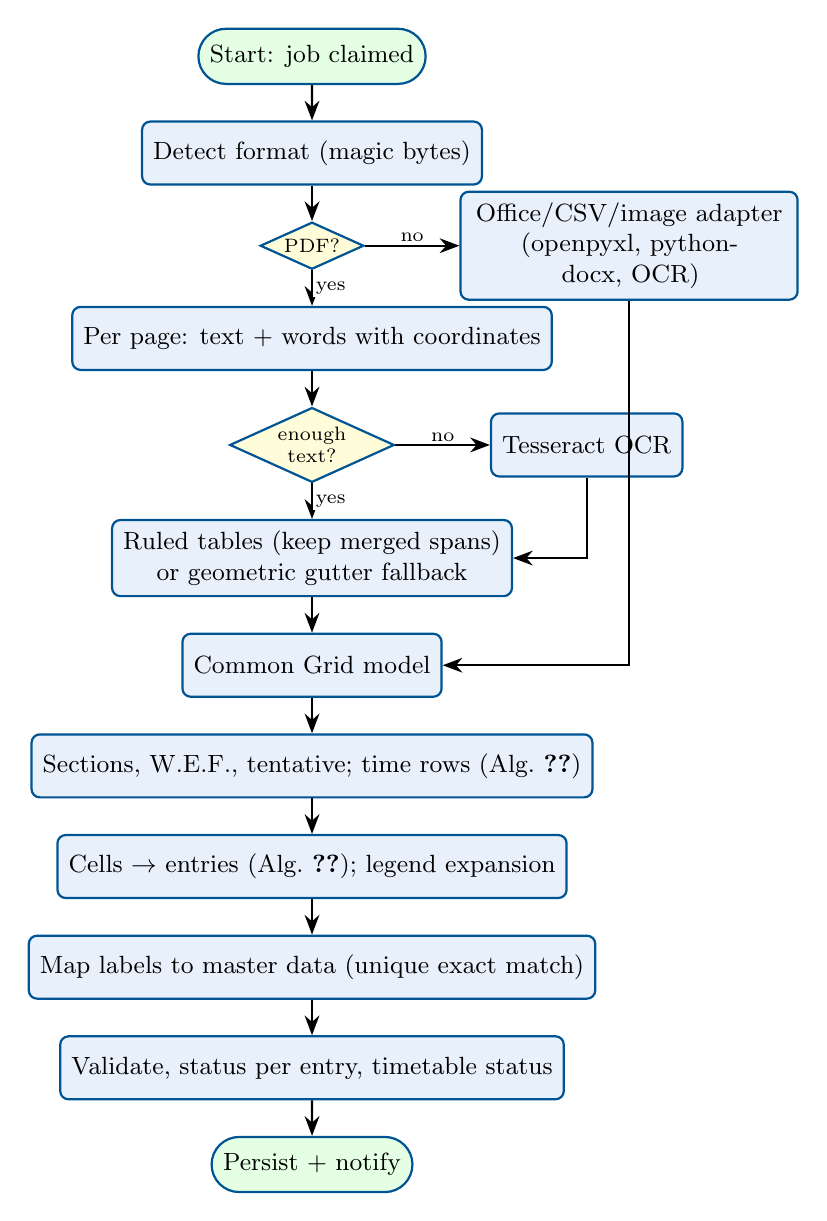
\begin{tikzpicture}[node distance=4.5mm]
\node[term] (s) {Start: job claimed};
\node[blk,below=of s] (a) {Detect format (magic bytes)};
\node[dec,below=of a] (d1) {PDF?};
\node[blk,right=12mm of d1,text width=40mm] (o) {Office/CSV/image adapter\\(openpyxl, python-docx, OCR)};
\node[blk,below=of d1] (b) {Per page: text + words with coordinates};
\node[dec,below=of b] (d2) {enough\\text?};
\node[blk,right=12mm of d2] (ocr) {Tesseract OCR};
\node[blk,below=of d2] (c) {Ruled tables (keep merged spans)\\or geometric gutter fallback};
\node[blk,below=of c] (g) {Common Grid model};
\node[blk,below=of g] (h) {Sections, W.E.F., tentative; time rows (Alg.~\ref{alg:time})};
\node[blk,below=of h] (i) {Cells $\rightarrow$ entries (Alg.~\ref{alg:cell}); legend expansion};
\node[blk,below=of i] (j) {Map labels to master data (unique exact match)};
\node[blk,below=of j] (k) {Validate, status per entry, timetable status};
\node[term,below=of k] (e) {Persist + notify};
\draw[arr] (s)--(a); \draw[arr] (a)--(d1); \draw[arr] (d1)--node[lbl,right]{yes}(b); \draw[arr] (d1)--node[lbl,above]{no}(o);
\draw[arr] (o.south) |- (g.east);
\draw[arr] (b)--(d2); \draw[arr] (d2)--node[lbl,right]{yes}(c); \draw[arr] (d2)--node[lbl,above]{no}(ocr);
\draw[arr] (ocr.south) |- (c.east);
\draw[arr] (c)--(g); \draw[arr] (g)--(h); \draw[arr] (h)--(i); \draw[arr] (i)--(j); \draw[arr] (j)--(k); \draw[arr] (k)--(e);
\end{tikzpicture}
\caption{Flowchart of the extraction pipeline}
\label{fig:flowextract}
\end{figure}

\begin{figure}[H]
\centering
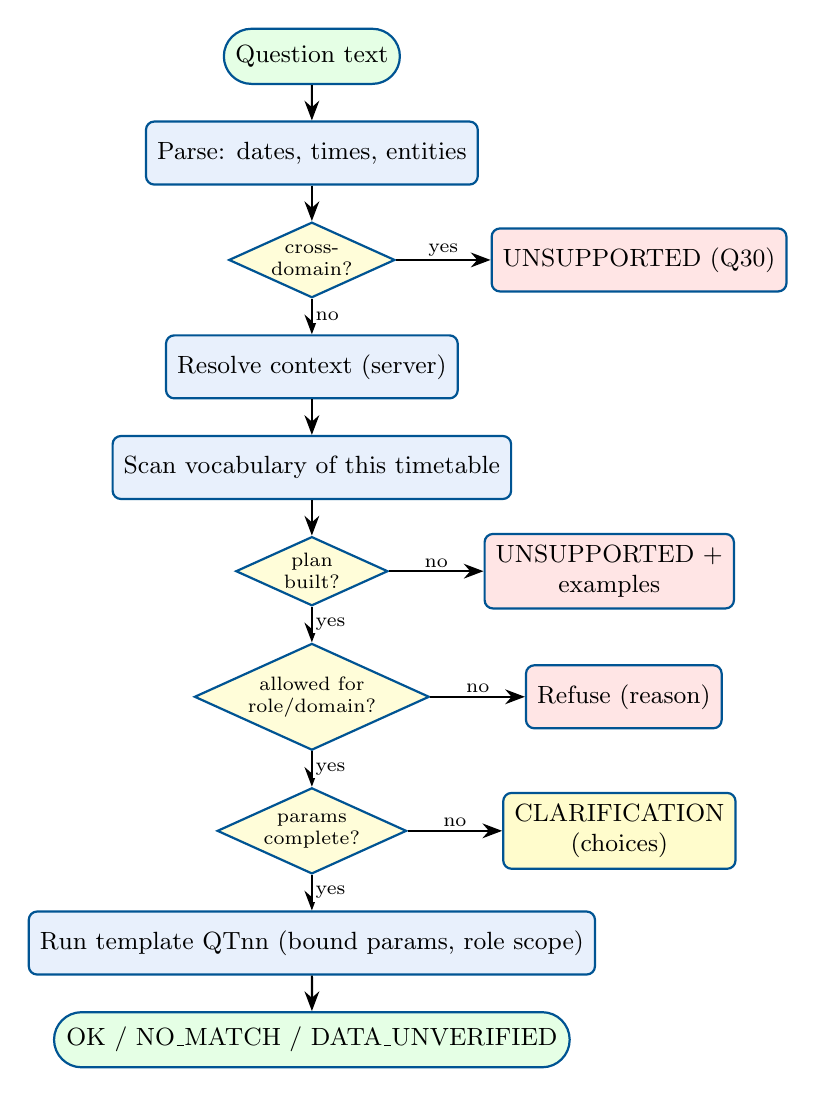
\begin{tikzpicture}[node distance=4.5mm]
\node[term] (s) {Question text};
\node[blk,below=of s] (p) {Parse: dates, times, entities};
\node[dec,below=of p] (x) {cross-\\domain?};
\node[blk,right=12mm of x,fill=red!10] (x1) {UNSUPPORTED (Q30)};
\node[blk,below=of x] (c) {Resolve context (server)};
\node[blk,below=of c] (v) {Scan vocabulary of this timetable};
\node[dec,below=of v] (k) {plan\\built?};
\node[blk,right=12mm of k,fill=red!10] (k1) {UNSUPPORTED +\\examples};
\node[dec,below=of k] (r) {allowed for\\role/domain?};
\node[blk,right=12mm of r,fill=red!10] (r1) {Refuse (reason)};
\node[dec,below=of r] (m) {params\\complete?};
\node[blk,right=12mm of m,fill=yellow!20] (m1) {CLARIFICATION\\(choices)};
\node[blk,below=of m] (t) {Run template QTnn (bound params, role scope)};
\node[term,below=of t] (e) {OK / NO\_MATCH / DATA\_UNVERIFIED};
\draw[arr] (s)--(p); \draw[arr] (p)--(x); \draw[arr] (x)--node[lbl,above]{yes}(x1); \draw[arr] (x)--node[lbl,right]{no}(c);
\draw[arr] (c)--(v); \draw[arr] (v)--(k); \draw[arr] (k)--node[lbl,above]{no}(k1); \draw[arr] (k)--node[lbl,right]{yes}(r);
\draw[arr] (r)--node[lbl,above]{no}(r1); \draw[arr] (r)--node[lbl,right]{yes}(m);
\draw[arr] (m)--node[lbl,above]{no}(m1); \draw[arr] (m)--node[lbl,right]{yes}(t); \draw[arr] (t)--(e);
\end{tikzpicture}
\caption{Flowchart of the query engine}
\label{fig:flowquery}
\end{figure}

\subsection{Data Structure Selection}
\begin{table}[H]
\centering
\caption{Data structures used and why}
\label{tab:ds}
\small
\begin{tabularx}{\textwidth}{@{}p{3.2cm}p{4.3cm}X@{}}
\toprule
\textbf{Data structure} & \textbf{Where} & \textbf{Reason}\\
\midrule
Hash map (dict) & Conflict groups keyed by (resource, key, day); page legend; vocabulary n-gram index & $O(1)$ average lookup and grouping, replacing $O(n^2)$ all-pairs comparison\\
Hash set & Seen conflict pairs; used tokens; role sets & De-duplication in $O(1)$\\
Sorted array + sweep & Entries per group sorted by start time & Early \texttt{break} when no later interval can overlap\\
2-D grid (list of rows of cells with span) & \texttt{Grid} model shared by all adapters & Natural model of a timetable; merged cells keep row/column span\\
Tree (parent pointer) & Batch hierarchy SE $\rightarrow$ SE-A $\rightarrow$ SE-A1 & A lab group inherits division classes by walking to the root ($O(\text{depth})$, depth $\le 3$)\\
Queue (FIFO) & \texttt{processing\_job} ordered by \texttt{created\_at} & Fair processing order; persistent across crashes\\
B-tree index & PostgreSQL composite indexes & $O(\log n)$ range scans on (timetable, day, start)\\
Search tree of assignments & Time-row backtracking (Alg.~\ref{alg:time}) & Explores consistent readings; pruned by ordering constraint\\
Immutable registry (tuple/dict) & Operations Q01--Q31, templates QT01--QT23, plan vocabulary & Closed set; unknown operations or plan values cannot be executed\\
\bottomrule
\end{tabularx}
\end{table}

\subsection{Algorithm Selection and Justification}
\begin{table}[H]
\centering
\caption{Alternatives considered for the key algorithms}
\label{tab:algsel}
\small
\begin{tabularx}{\textwidth}{@{}p{2.8cm}XXp{3cm}@{}}
\toprule
\textbf{Problem} & \textbf{Alternative} & \textbf{Chosen} & \textbf{Justification}\\
\midrule
Clash detection & All pairs, $O(n^2)$ & Group by resource (hash) + sort + sweep & Same result, $O(n\log n + m)$; simpler to explain intended-overlap rules per group\\
Clash detection & Interval tree & Sorted sweep & Groups are small (tens of entries); a tree adds code without measurable gain\\
Time labels & Trust printed a.m./p.m.\ & Constrained backtracking with uniqueness & Printed markers are wrong in the real PDF; uniqueness gives provable certainty\\
Question understanding & LLM text-to-SQL; trained intent classifier; one fixed rule per question & Compositional query plan (independent rules per piece) + vocabulary scan + compiled templates & Deterministic, explainable, injection-safe, no training data or API cost~\cite{androutsopoulos1995,pedro2023}\\
Entity matching & Fuzzy auto-select & Exact $\rightarrow$ unique word $\rightarrow$ fuzzy \emph{suggestions} & Avoids silently picking the wrong professor\\
Job distribution & Redis/RabbitMQ & PostgreSQL \texttt{SKIP LOCKED} & One less service; job creation is transactional with the upload\\
Table extraction & Deep-learning table detector & PyMuPDF ruled tables + geometric fallback & Text PDFs are exact; no GPU; explainable failures\\
\bottomrule
\end{tabularx}
\end{table}

\subsection{Time Complexity Analysis}
Let $n$ be the number of entries in a timetable, $r$ the rows of a grid section, $w$ the words in a
question, $|V|$ the vocabulary size, $m$ the number of overlapping pairs reported, and $R$ the number of rooms.

\begin{table}[H]
\centering
\caption{Time complexity of critical operations}
\label{tab:timecx}
\small
\begin{tabularx}{\textwidth}{@{}p{4.3cm}p{3.5cm}X@{}}
\toprule
\textbf{Operation} & \textbf{Complexity} & \textbf{Remarks}\\
\midrule
Time-row resolution & worst $O(4^{r})$, bounded by 64 solutions; typical $O(r)$ & $r \le 12$ rows, $\le 4$ readings each; the ordering constraint prunes almost all branches\\
Cell parsing (whole PDF) & $O(C \cdot \ell)$ & $C$ cells, $\ell$ tokens per cell; legend lookup $O(1)$\\
Conflict detection & $O(n \log n + m)$ average & Hash grouping $O(n)$, sort per group, sweep with early break. Worst case (all overlapping in one group) $O(n^2)$\\
Division vs sub-group check & $O(d^2)$ per day & $d$ entries with batch label on a day; acceptable for $d \approx 100$, see Section 5.8\\
Parse + classify question & $O(w)$ & Fixed number of regular expressions\\
Build query plan & $O(w)$ & One pass of a fixed set of piece rules (operation, kind, window, sort)\\
Execute composed plan & $O(D\log n + k\log k)$ & $D \leq 7$ day range scans on the index; $k$ matching entries sorted for slots, first/last and per-day sums\\
Vocabulary scan & $O(4w)$ lookups & n-gram sizes 4..1, hash index built in $O(|V|)$\\
Next class & $O(H \log n)$ & At most $H{=}7$ index range scans\\
Free rooms & $O(\log n + k + R)$ & $k$ entries at that time, set difference over $R$ rooms\\
Job claim & $O(\log J)$ & Index on (status, created\_at)\\
\bottomrule
\end{tabularx}
\end{table}

\subsection{Space Complexity Analysis}
Extraction holds one document's grid in memory: $O(C)$ cells plus $O(n)$ entries, a few megabytes
for a 10-page PDF. OCR is the largest consumer (one page image at native resolution at a time, so
memory is bounded by one page). Conflict detection uses $O(n)$ for the hash groups and $O(m)$ for
results. The backtracking stores at most 64 assignments of length $r$, so $O(64r)$. The query
vocabulary is $O(|V|)$ per request (about 200 labels for the real timetable). The database stores one
row per entry, so 570 rows (453 classes plus breaks and activities) for the real PDF. The whole
development database with this timetable, users and history measured \textbf{12~MB}.

\subsection{Optimisation Opportunities}
\begin{itemize}
\item \textbf{Done -- N+1 queries removed:} loading related course/staff/room/batch rows eagerly cut
      the number of SQL statements per search from about 50 to about 25 (Section~8.9).
\item \textbf{Done -- batched vocabulary loading:} one query per entity type instead of one per label.
\item \textbf{Possible -- division-pair sweep:} the $O(d^2)$ loop can use the same sort-and-break
      sweep as the main groups.
\item \textbf{Possible -- vocabulary cache:} cache the vocabulary per (timetable, data\_version); it
      changes only on correction or activation.
\item \textbf{Possible -- parallel page extraction:} pages are independent, so OCR of scanned PDFs
      could use a process pool.
\end{itemize}

\newpage

\section{Subject-Wise Engineering Concepts and APNI Leap Alignment}
This chapter shows how concepts from Semesters I--IV were applied in the project. Every claim points
to code in the repository or to a test, so it can be checked.

\subsection{Software Engineering}
\begin{itemize}
\item \textbf{Process model:} incremental. Each phase (requirements $\rightarrow$ back-end foundation
      $\rightarrow$ extraction $\rightarrow$ query engine $\rightarrow$ app $\rightarrow$ testing
      $\rightarrow$ deployment) produced a working, tested increment and a commit
      (Section~7.8)~\cite{sommerville}.
\item \textbf{Requirement traceability:} every functional requirement (FR-01 \ldots FR-19) maps to
      modules (Table~\ref{tab:modules}) and test cases (Table~\ref{tab:testcases}). Conflicts between the
      source specifications were recorded with their resolution (\texttt{docs/01-requirements-and-decisions.md},
      C-01 \ldots C-10, D-01 \ldots D-20).
\item \textbf{Modularity and separation of concerns:} routers $\rightarrow$ services $\rightarrow$
      query/extraction $\rightarrow$ models. Security policy lives in one file
      (\texttt{security/policy.py}), and domain separation in one adapter (\texttt{services/domains.py}).
\item \textbf{State management (client):} server state in TanStack Query (cache, invalidation on
      activation), authentication state in a React context, form state in React Hook Form with Zod schemas.
\item \textbf{Exception handling:} typed application errors mapped to one JSON error envelope; the
      worker separates retryable from deterministic failures.
\item \textbf{Version control:} Git with a feature branch and descriptive commit messages (Section~7.8).
\item \textbf{Quality:} static typing (Pydantic, TypeScript \texttt{strict}), 178 + 20 automated tests,
      end-to-end tests, a security audit with prioritised findings (P0--P2).
\end{itemize}

\subsection{Computer Networks}
\begin{itemize}
\item \textbf{Architecture:} client--server over TCP/IP. Many clients (phones and browsers) talk to
      one logical server over HTTPS (HTTP/1.1 over TLS over TCP, port 443). The database is reached over
      TCP port 5432 on a private network.
\item \textbf{Protocol and message format:} REST resources under \texttt{/api/v1}; JSON request and
      response bodies; \texttt{multipart/form-data} for uploads; standard status codes (200, 401, 403,
      404, 413, 422, 429). Search answers always use one envelope
      (\texttt{status}, \texttt{intent}, \texttt{results}, \texttt{warnings}, \texttt{clarification}).
\item \textbf{Connection management:} stateless requests with bearer tokens; keep-alive handled
      by the HTTP client; a database connection pool per API process.
\item \textbf{Error recovery:} client timeouts; automatic retry only for idempotent reads;
      \emph{single-flight} token refresh, where many requests that receive 401 at the same time share
      one refresh call (tested in Jest); offline detection with NetInfo and a cached last-known
      institutional timetable.
\item \textbf{Real bug found:} the web build checked connectivity with an HTTP \texttt{HEAD /}
      request, which the server answered with 405, so the app believed it was offline and stayed
      on ``Loading\ldots''. The server now accepts \texttt{HEAD} for the web routes (Section~9.9).
\item \textbf{Concurrency:} several Uvicorn worker processes each serve concurrent requests, so many
      clients are served at once (Section~8.4).
\end{itemize}

\subsection{Database Management Systems}
\begin{itemize}
\item \textbf{ER modelling and normalisation} to 3NF (Section~4.6), with a justified provenance
      denormalisation (raw labels).
\item \textbf{Keys and constraints:} UUID and identity PKs; FKs including \emph{composite} FKs
      that make a user's preference point only to their own personal timetable; CHECK constraints (day
      1--7, end $>$ start, status enums, single-row settings); \emph{partial unique} indexes (one open
      academic placement per student; one active academic year; idempotent uploads per client request id).
\item \textbf{Indexing and query optimisation:} composite B-tree indexes led by
      \texttt{timetable\_id}; eager loading removed N+1 queries (about 50 $\rightarrow$ about 25
      statements per search).
\item \textbf{Transactions and concurrency control:} activation locks the settings row
      (\texttt{SELECT \ldots{} FOR UPDATE}); promotion locks student rows in a stable order to avoid
      deadlocks; job claiming uses \texttt{FOR UPDATE SKIP LOCKED}; each request runs in one
      transaction, so it sees one consistent snapshot.
\item \textbf{Schema migration:} Alembic versioned migrations (0001 schema, 0002 reference data, 0003
      time-uncertainty flag).
\item \textbf{Security:} parameterised queries only, so no SQL is ever built from user text.
\end{itemize}

\subsection{Operating Systems}
\begin{itemize}
\item \textbf{Processes:} the API runs as several OS processes (Uvicorn workers); extraction runs in a
      separate worker process, so CPU-heavy OCR cannot starve request handling. On the free tier the
      worker runs as a background \emph{thread} in the same process instead.
\item \textbf{Producer--consumer:} the API (producer) inserts jobs and workers (consumers) remove them
      from a shared, persistent FIFO queue: the \texttt{processing\_job} table.
\item \textbf{Synchronisation:} database row locks act as the mutual-exclusion mechanism.
      \texttt{SKIP LOCKED} gives non-blocking acquisition, which is like a \emph{try-lock}, so idle
      workers never wait on a busy row.
\item \textbf{Deadlock avoidance:} resources (student rows) are always locked in the same order,
      which breaks the circular-wait condition.
\item \textbf{Fault tolerance:} heartbeat timestamps detect crashed workers, a job whose heartbeat is
      older than 10 minutes is re-claimed, and the maximum attempt count prevents infinite retry loops.
\item \textbf{Scheduling:} jobs are served first-come-first-served (\texttt{ORDER BY created\_at}). The
      OS scheduler time-slices request handling across processes. Section~8.5 discusses the
      measurements. We did not need a custom Round-Robin scheduler, because jobs are rare and short (under 2~s).
\item \textbf{Resource limits:} upload size (15~MB) and page count (30), and a timeout on the
      LibreOffice conversion subprocess.
\end{itemize}

\subsection{Data Structures}
Hash maps for grouping and legend/vocabulary lookup, sets for de-duplication, sorted arrays with a
sweep for interval overlap, a 2-D grid with spans for the timetable, a parent-pointer tree for the
batch hierarchy, a FIFO queue for jobs and B-tree indexes in the database (Table~\ref{tab:ds}).

\subsection{Design and Analysis of Algorithms}
\begin{itemize}
\item \textbf{Backtracking with pruning} for time-row resolution, with a uniqueness test for
      certainty (Algorithm~\ref{alg:time}).
\item \textbf{Divide by key, sort and sweep} for interval-overlap detection, $O(n\log n + m)$
      instead of $O(n^2)$ (Algorithm~\ref{alg:conflict})~\cite{cormen2009}.
\item \textbf{Greedy longest-match} n-gram scanning for entity mentions.
\item \textbf{Compositional semantic parsing}: independent rules for operation, filters, time window and
      sort combine into a query plan, which is then compiled into queries (a small query algebra:
      selection by day and filters, then aggregation by count, sum, min/max or group-by-day; Algorithm~\ref{alg:plan}).
\item \textbf{Interval algebra} for overlap and free-time computation~\cite{allen1983}.
\item \textbf{Correctness argument (conflicts):} after sorting by start time, if $g_j.\mathit{start}
      \geq g_i.\mathit{end}$ then every later $g_k$ ($k>j$) also has $g_k.\mathit{start} \geq g_i.\mathit{end}$,
      so it cannot overlap $g_i$. The early break therefore never misses a conflict.
\end{itemize}

\subsection{Cloud Computing}
\begin{itemize}
\item \textbf{Service model:} Platform-as-a-Service (Render) running our \textbf{Docker} container,
      plus a managed PostgreSQL database (Database-as-a-Service).
\item \textbf{Infrastructure as code:} \texttt{render.yaml} blueprint declares the web service, the
      database and environment variables. A push to the branch triggers build and deploy (continuous deployment).
\item \textbf{Configuration and secrets:} 12-factor style environment variables; the secret key is
      generated by the platform and the demo password is entered at deploy time, so nothing secret is
      in Git.
\item \textbf{Availability and scaling:} a health-check endpoint; the stateless API scales
      horizontally; the free tier sleeps after 15 minutes idle (a cost/availability trade-off).
\end{itemize}

\subsection{Mapping of Subjects to Project Implementation}
\begin{longtable}{@{}p{2.2cm}p{4cm}p{3.6cm}p{5.1cm}@{}}
\caption{Mapping of Semester I--IV subjects to the project}\label{tab:mapping}\\
\toprule
\textbf{Subject} & \textbf{Concept applied} & \textbf{Project module} & \textbf{Evidence}\\
\midrule
\endfirsthead
\toprule
\textbf{Subject} & \textbf{Concept applied} & \textbf{Project module} & \textbf{Evidence}\\
\midrule
\endhead
DBMS & Normalisation, PK/FK, CHECK, partial unique indexes & Schema (\texttt{models.py}, migrations) & ER diagram Fig.~\ref{fig:er}; Table~\ref{tab:schema}\\
DBMS & Indexing, N+1 elimination & Query templates & 50 $\rightarrow$ 25 statements per search; latency results (Ch.~8)\\
DBMS & Transactions, row locking & Activation, promotion & Concurrent activation/promotion tests (one wins, no corruption)\\
Operating Systems & Producer--consumer, mutual exclusion (try-lock) & Worker, job queue & \texttt{SKIP LOCKED} claim; worker retry test\\
Operating Systems & Processes vs threads, deadlock avoidance & API workers, promotion & Load test with 4 processes; ordered locking\\
Computer Networks & Client--server, HTTP/REST, JSON, TLS & API, app client & OpenAPI spec (\texttt{docs/openapi.json}); e2e tests\\
Computer Networks & Error recovery, single-flight refresh & \texttt{api/client.ts} & Jest test with concurrent 401s\\
Data Structures & Hash maps, sets, trees, queues, grids & Extraction, conflicts, vocabulary & Code; Table~\ref{tab:ds}\\
Analysis of Algorithms & Backtracking, sort + sweep, complexity & Time parser, conflicts & Alg.~\ref{alg:time}, \ref{alg:conflict}; Table~\ref{tab:timecx}\\
Software Engineering & SRS, traceability, testing, Git & Whole project & FR table, test-case table, commit history\\
Discrete Mathematics & Sets, relations, intervals, predicate logic & Clash rule, role scopes & $a.s<b.e \wedge b.s<a.e$; RBAC matrix\\
Programming (Python, JS) & OOP, typing, async UI & Back end, app & 10.5k lines Python, 5.5k lines TypeScript\\
Cloud Computing & PaaS, Docker, IaC, CD & Deployment & \texttt{render.yaml}, \texttt{deploy/render.Dockerfile}; live demo\\
Information Security (applied) & Hashing, tokens, RBAC, OWASP & \texttt{app/security} & Auth tests; P0 fix verified with 9 checks\\
\bottomrule
\end{longtable}

\newpage

\section{Implementation and Module-Wise Coding}

\subsection{Development Environment}
\begin{itemize}
\item \textbf{Languages:} Python 3.13 (back end, about 10{,}500 lines in \texttt{backend/app}), TypeScript
      in strict mode (app, about 5{,}500 lines in \texttt{mobile/src}), SQL (migrations, templates).
\item \textbf{Frameworks and libraries:} FastAPI, SQLAlchemy 2.1, Alembic, Pydantic v2, PyMuPDF,
      pytesseract, openpyxl, python-docx, RapidFuzz, argon2-cffi, PyJWT; Expo SDK 58, React Native 0.88,
      Expo Router, TanStack Query, React Hook Form, Zod.
\item \textbf{Tools:} VS Code, Git/GitHub, PostgreSQL 16, Docker, Expo Go, Chrome DevTools, pytest,
      Jest, Playwright, Render.
\item \textbf{Operating systems:} Windows and Linux laptops for development; Android and iPhone for device testing.
\end{itemize}

\subsection{Overall Implementation Strategy}
The design was translated into software \emph{risk first}, from the inside out:
\begin{enumerate}
\item \textbf{Foundation:} schema, migrations, authentication, RBAC and admin master data, so every
      later feature was secure from the start.
\item \textbf{Extraction engine:} the riskiest part, built and tuned on the real college PDF early.
\item \textbf{Query engine:} the intent registry and templates, tested intent by intent (Q01--Q30).
\item \textbf{Mobile app} on top of a stable, documented API (OpenAPI).
\item \textbf{Hardening:} concurrency tests, a security audit, the real-PDF rules from the college,
      laptop/web support, the SDK upgrade and free cloud deployment.
\end{enumerate}
Each step ended with all tests passing and a commit (Table~\ref{tab:commits}).

\subsection{Module-Wise Implementation}
\paragraph{M1. Authentication and RBAC (\texttt{app/security}, \texttt{services/auth.py}).}
\emph{Input/Output:} credentials $\rightarrow$ access token (15 min) and refresh token (30 days, stored only as a hash).
\emph{Logic:} Argon2id verification; on refresh, the old token is revoked and a new one is issued in
the same family, and reuse of a revoked token revokes the family. \texttt{load\_principal} reads roles,
staff profile and academic placement from the database on every request. \texttt{policy.py} maps
roles to data scopes (batch, department, college).
\emph{Tests:} 15 tests in \texttt{test\_auth.py} (rotation, reuse detection, suspension, role change, rate limit).

\paragraph{M2. Upload and archive (\texttt{services/uploads.py}, \texttt{storage.py}).}
\emph{Input:} multipart file plus metadata. \emph{Logic:} extension allow-list and magic-byte
check (\texttt{extraction/filetypes.py}), size and page limits, atomic private write (mode 0600),
SHA-256 for duplicate detection, archive row and job row in one transaction, idempotency via
\texttt{client\_request\_id}. \emph{Output:} timetable id in state \textsc{Queued}.
\emph{Tests:} \texttt{test\_uploads\_and\_domains.py} (13).

\paragraph{M3. Extraction (\texttt{app/extraction}, 11 files).}
\texttt{pdf.py} (PyMuPDF tables and words), \texttt{geometric.py} (gutter-based columns),
\texttt{ocr.py} (Tesseract), \texttt{office.py} (XLSX/CSV/DOCX, LibreOffice for legacy formats)
$\rightarrow$ \texttt{model.py} (Grid) $\rightarrow$ \texttt{sections.py}, \texttt{timeparse.py},
\texttt{gridparse.py}, \texttt{cellparse.py} $\rightarrow$ \texttt{validate.py} $\rightarrow$
\texttt{pipeline.py}. The parser version (\texttt{tt-grid-parser/1.2.0}) is stored with every entry.
\emph{Tests:} 24 extraction tests and 14 regression tests on the real PDF.

\paragraph{M4. Worker (\texttt{app/worker.py}).}
Claims jobs (Listing~\ref{lst:claim}), runs the pipeline, persists entries, computes the timetable
status, notifies the uploader, and retries unexpected failures. It can run as a separate process
(\texttt{python -m app.worker}) or as a thread inside the API on the free tier.

\paragraph{M5. Query engine (\texttt{app/query}).} Files \texttt{nlp.py}, \texttt{vocab.py}, \texttt{registry.py}, \texttt{engine.py} and \texttt{templates.py}.
Implements Algorithm~\ref{alg:query}. \texttt{registry.py} declares the 30 intents with their allowed
domains, roles, required parameters and templates. \texttt{templates.py} holds the 22 parameterised
SQLAlchemy queries. \emph{Tests:} 57 tests in \texttt{test\_query\_engine.py}, including SQL-injection text
and unknown parameters.

\paragraph{M6. Conflicts (\texttt{services/conflicts.py}).}
Implements Algorithm~\ref{alg:conflict} and returns \textsc{Confirmed}/\textsc{Possible} conflicts,
scoped to the HOD's department. \emph{Test:} the real-PDF test asserts that exactly the two genuine clashes
are reported.

\paragraph{M7. Academics and administration.} Files \texttt{services/academics.py}, \texttt{users.py} and \texttt{api/v1/admin.py}.
Fresher registration without duplicates, promotion with preview and confirm (all or nothing, history
preserved), and master data CRUD with validation. \emph{Tests:} 13 in \texttt{test\_academics\_admin.py}, including
concurrent promotions.

\paragraph{M8. Mobile and web client (\texttt{mobile/src}).}
Described in Section~7.4. \emph{Tests:} 18 Jest tests and Playwright end-to-end tests.

\subsection{Front-End Implementation}
The app has 26 screens organised with Expo Router (file-based routing):
\begin{itemize}
\item \textbf{Auth stack:} welcome, login, account activation, forgot password.
\item \textbf{Tabs:} Home (role dashboard), Ask (NL search), Timetable (week strip and day timeline),
      Archives, Admin (Admins only; hiding the tab is cosmetic because the server enforces access), Profile.
\item \textbf{Stack screens:} class details, timetable details (extraction summary, sections),
      review \& correct, upload, conflicts, monitoring, notifications, admin tools (users, new user,
      promotion, master data, institution settings, jobs, audit log).
\end{itemize}
\textbf{Forms} use React Hook Form with Zod schemas (e.g.\ e-mail format, password rules, room code).
\textbf{Navigation} is file-based. \textbf{State}: server data in TanStack Query with keys per domain
and timetable, invalidated when the official timetable changes. A
\textbf{College/Personal toggle} switches the domain, with a different accent colour so users always
know which data they see. \textbf{Accessibility}: light/dark themes, large tap targets, labels for
screen readers. On a wide laptop screen the app is shown as a centred column. The web session is kept in
\texttt{sessionStorage} (cleared when the tab closes), and on phones in the Keychain/Keystore.

\subsection{Back-End Implementation}
\begin{itemize}
\item \textbf{76 REST endpoints} in six routers: \texttt{auth}, \texttt{me}, \texttt{timetables},
      \texttt{search}, \texttt{notifications}, \texttt{admin}. The OpenAPI specification is generated
      automatically (\texttt{docs/openapi.json}).
\item \textbf{Request processing:} middleware adds a request id and JSON logging; dependencies
      authenticate and load the principal; Pydantic validates bodies; services hold business logic; the
      error handler converts exceptions to the envelope.
\item \textbf{Search context:} \texttt{services/context.py} decides the domain (request hint
      $\rightarrow$ remembered $\rightarrow$ institutional), the timetable (explicit archive
      $\rightarrow$ remembered archive $\rightarrow$ primary), verifies ownership and usability, and
      computes ``now'' in the user's time zone.
\item \textbf{Static web app:} in the deployed image the same FastAPI process serves the exported web
      app, so phone and laptop use one HTTPS origin.
\end{itemize}

\subsection{Database Implementation}
31 tables are created by Alembic migrations. Templates are SQLAlchemy Core/ORM expressions with
bound parameters. A representative template (QT08, next class) is:
\begin{lstlisting}[language=Python,caption={Template QT08 (simplified): next class within a scope},label=lst:qt08]
stmt = (select(E)
        .where(E.timetable_id == ctx.timetable_id,
               E.entry_kind == "CLASS",
               E.verification_status != "REJECTED",
               E.time_uncertain.is_(False),
               or_(E.class_date == day, and_(E.class_date.is_(None),
                                             E.day_of_week == day.isoweekday())),
               E.start_time > after,
               scope_filter(ctx))          # batch + parent batch, or staff id
        .order_by(E.start_time)
        .limit(1))
\end{lstlisting}
Connectivity: one SQLAlchemy engine per process with a connection pool (\texttt{psycopg} 3 driver);
each request gets a session that commits or rolls back as one transaction.

\subsection{Communication and Concurrency Implementation}
\begin{itemize}
\item \textbf{Client--server:} \texttt{mobile/src/api/client.ts} adds the bearer token, applies
      timeouts, retries idempotent GETs, and performs a \emph{single-flight} refresh: the first 401
      starts one refresh call and all other failing requests wait for the same promise, then retry.
\item \textbf{Concurrent clients:} several Uvicorn processes; each request is independent
      (stateless), with its own database transaction.
\item \textbf{Synchronisation:} activation and preference changes use \texttt{SELECT \ldots{} FOR
      UPDATE}; job claiming uses \texttt{SKIP LOCKED}; uploads are idempotent through a partial unique index;
      the rate limiter uses a lock-protected in-process sliding window.
\item \textbf{Recovery:} job heartbeat and re-claim; maximum attempts; the client shows the cached
      institutional timetable with ``last refreshed'' time when offline.
\end{itemize}

\subsection{Git Repository Setup}
\begin{itemize}
\item \textbf{Repository URL:} \url{\RepoURL}
\item \textbf{Structure:} \texttt{backend/} (app, alembic, tests), \texttt{mobile/} (src, \_\_tests\_\_, e2e),
      \texttt{docs/} (13 documents + OpenAPI), \texttt{deploy/} (Render image), \texttt{scripts/}
      (dev script, Windows one-click start, load smoke), \texttt{report/} (this report and poster),
      \texttt{render.yaml}, \texttt{docker-compose.yml}.
\item \textbf{Branching strategy:} \texttt{main} is the stable branch; development happens on a feature
      branch that is merged through a pull request after review. The Render demo deploys from the
      development branch, so every push updates the demo.
\item \textbf{Commit message convention:} an imperative summary of what changed and why, naming the
      scope (e.g.\ ``Query engine: intent registry Q01--Q30 \ldots''), with the details in the body.
\end{itemize}

\begingroup\small
\begin{longtable}{@{}p{1.5cm}p{1.9cm}p{9.0cm}p{2.3cm}@{}}
\caption{Development history (commits on the development branch)}\label{tab:commits}\\
\toprule
\textbf{Commit} & \textbf{Date} & \textbf{Message (summary)} & \textbf{Files / lines}\\
\midrule
\endfirsthead
\toprule
\textbf{Commit} & \textbf{Date} & \textbf{Message (summary)} & \textbf{Files / lines}\\
\midrule
\endhead
\texttt{0dfda92} & 2026-10-09 & Backend foundation: schema, migrations, auth, RBAC, admin master data & 46 / +5164\\
\texttt{bc917fb} & 2026-10-09 & Extraction engine (PDF/OCR/Excel/CSV/Word/images), worker, archives, review, conflicts & 30 / +3841\\
\texttt{47e3d89} & 2026-10-09 & Query engine: intent registry Q01--Q30, templates QT01--QT22, entity resolution, clarification & 17 / +3026\\
\texttt{1aa651d} & 2026-10-09 & Expo mobile app: role dashboards, NL search, weekly timetable, archives, uploads, review, admin; Jest + Playwright & 72 / +18618\\
\texttt{f028feb} & 2026-10-09 & Academic/admin/conflict/concurrency tests, batched vocabulary loading, load smoke script & 7 / +353\\
\texttt{4f3528b} & 2026-10-09 & Documentation, OpenAPI export, Docker/compose, EAS profiles, pinned requirements & 23 / +7345\\
\texttt{bb81091} & 2026-10-09 & Tune extraction on the college's real timetable PDF (parser 1.1.0) & 13 / +508\\
\texttt{dc12b25} & 2026-10-09 & Apply the college's timetable rules; real-PDF seed; phone guide & 31 / +1106\\
\texttt{710e679} & 2026-10-14 & College seed: one student login per lab group & 3 / +24\\
\texttt{fce3644} & 2026-10-21 & Run the app in a laptop browser; one-click Windows start & 7 / +129\\
\texttt{e8f74c3} & 2026-10-21 & Hide admin review notices from students; fix archive banner & 12 / +102\\
\texttt{326b8e6} & 2026-10-25 & Upgrade the app to Expo SDK 58 & 8 / +9018 (lockfile)\\
\texttt{8093f09} & 2026-10-25 & Free online demo (Render) + fix account takeover via password reset (P0-1) & 25 / +444\\
\bottomrule
\end{longtable}
\endgroup

\paragraph{Contribution of individual group members.}
\begin{table}[H]
\centering
\caption{Contribution of group members (to be confirmed by the group and guide)}
\label{tab:contrib}
\small
\begin{tabularx}{\textwidth}{@{}p{3.6cm}X@{}}
\toprule
\textbf{Member} & \textbf{Main contributions}\\
\midrule
\StudentA{} (\UIDA) & \textit{[e.g.\ back-end foundation, query engine, deployment]}\\
\StudentB{} (\UIDB) & \textit{[e.g.\ extraction pipeline and real-PDF tuning]}\\
\StudentC{} (\UIDC) & \textit{[e.g.\ mobile app screens and UI design]}\\
\StudentD{} (\UIDD) & \textit{[e.g.\ testing, documentation, report and poster]}\\
\bottomrule
\end{tabularx}
\end{table}

\subsection{Integration of Modules}
Modules communicate only through defined interfaces: the app uses the REST API; routers call
services; services call the query engine or put jobs in the queue; the worker calls the extraction
pipeline and writes through the same models. Integration was verified at three levels:
(1) back-end integration tests that upload a file, run the worker, activate the timetable and query it
through the API; (2) the college seed test, which runs the real PDF through the whole pipeline and then
asks questions as students, faculty, HOD and Admin; (3) Playwright end-to-end tests that drive the real
UI against the real API, including uploading a PDF through the file picker and waiting for the worker.

\subsection{Implementation Challenges and Resolutions}
\begin{longtable}{@{}p{4.2cm}p{4.6cm}p{6.2cm}@{}}
\caption{Implementation challenges and resolutions}\label{tab:challenges}\\
\toprule
\textbf{Challenge} & \textbf{Cause} & \textbf{Resolution}\\
\midrule
\endfirsthead
\toprule
\textbf{Challenge} & \textbf{Cause} & \textbf{Resolution}\\
\midrule
\endhead
Noon row printed as ``12.15 a.m.\ to 01.15 p.m.'' & Typing error in the source PDF & Accept midday only when proven by both neighbouring rows (Algorithm~\ref{alg:time})\\
Stacked lab cells (A1--A4 in one cell) & Four sub-groups share one grid cell & Line grouping by sub-group token; each becomes its own entry with its own room/teacher\\
Legends split across columns, codes missing from legend & Page layout & Page-local legend parser; unknown codes kept as written, with an INFO note (not an error)\\
Combined B.E.\ electives across divisions A--D & One page serves four divisions & Map to a common parent batch so all B.E.\ divisions see it\\
LLC slots with no teacher or room & Co-curricular course & Treat as a valid class without teacher/room; app hides empty fields\\
542 raw overlaps & Parallel labs and electives are intended & Intended-overlap rules $\rightarrow$ 2 genuine clashes\\
Slow searches (about 50 SQL statements) & N+1 lazy loading of related rows & Eager loading and batched vocabulary $\rightarrow$ about 25\\
Web app stuck on ``Loading\ldots'' in production & Connectivity probe used \texttt{HEAD /}, server returned 405 & Accept \texttt{GET} and \texttt{HEAD} on web routes; regression test\\
Account takeover risk (P0-1) & Password-reset code could be returned/logged in non-dev configuration & Never return or log codes in production; 9 verification checks\\
Expo Go on iPhone required SDK 58 & Store Expo Go supports only the newest SDK & Upgraded to SDK 58 / RN 0.88; fixed type changes; mocked icon fonts in Jest\\
Free hosting allows one service & Render free tier & In-process worker thread using the same \texttt{SKIP LOCKED} claim; static web app served by FastAPI\\
PowerShell blocked \texttt{npx} on Windows & Execution policy & Documented \texttt{npx.cmd} / policy change; one-click \texttt{start-windows.bat}\\
\bottomrule
\end{longtable}

\newpage

\section{Scalability, Performance and Resource Management}
\noindent\fbox{\parbox{\dimexpr\textwidth-2\fboxsep-2\fboxrule}{\small
\textbf{Tested vs.\ projected.} All numbers in this chapter labelled \emph{measured} were collected by us
on the development machine described in Section~8.6, with the real college timetable loaded. Numbers
labelled \emph{projected} are estimates and have not been tested on production hardware.}}

\subsection{Scalability Requirements}
\begin{table}[H]
\centering
\caption{Expected scale of one institute (projected)}
\label{tab:scale}
\small
\begin{tabularx}{\textwidth}{@{}Xp{6cm}@{}}
\toprule
\textbf{Quantity} & \textbf{Expected value}\\
\midrule
Registered users (students + staff) & 2{,}000--3{,}000\\
Batches / lab groups & 50--100 (real PDF: 46)\\
Class entries per official timetable & 500--1{,}000 (real PDF: 453 classes, 570 rows)\\
Timetable versions per semester & 3--10\\
Peak concurrent users (e.g.\ just after a timetable change) & 50--200\\
Peak request rate & 20--60 requests/s (a few requests per active user per minute)\\
Uploads & a few per week; each $\leq$ 15 MB, $\leq$ 30 pages\\
\bottomrule
\end{tabularx}
\end{table}

\subsection{Workload and Load Model}
The load test simulates students using the app at the same time:
\begin{itemize}
\item $N \in \{1, 2, 4, 8, 16, 32\}$ concurrent clients (threads), each logged in as a
      \emph{different} real student account (37 accounts, one per lab group).
\item Each client sends 30 search requests back-to-back with no think time (closed-loop, worst case),
      cycling through five realistic questions: ``What is my next class?'', ``What are my classes on
      Monday?'', ``Do I have classes after lunch on Tuesday?'', ``Which rooms are free at 10~am
      today?'' and ``Find all DBMS classes''.
\item Total requests per run $= 30N$ (30 to 960).
\item Every response is checked: HTTP 200 with \texttt{OK}/\texttt{NO\_MATCH}, or the expected 422
      clarification. (The M.Tech.\ page has no lunch row, so ``after lunch'' correctly asks for a time.)
\end{itemize}

\subsection{Resource Utilisation (measured)}
\begin{table}[H]
\centering
\caption{Measured resource utilisation}
\label{tab:resources}
\small
\begin{tabularx}{\textwidth}{@{}p{5.4cm}p{3cm}X@{}}
\toprule
\textbf{Resource} & \textbf{Value} & \textbf{How measured}\\
\midrule
Memory per API worker process (after load test) & 113--116 MB & \texttt{ps -o rss}, 4 workers\\
Peak memory, extraction of the 10-page PDF & 82 MB & \texttt{getrusage} max RSS\\
Database size (one timetable, 91 users, history) & 12 MB & \texttt{pg\_database\_size}\\
Entry table incl.\ indexes (570 rows) & 592 kB & \texttt{pg\_total\_relation\_size}\\
Original PDF stored & 420 kB & file size\\
CPU during 32-client test & $\approx$76\% of 4 cores & process CPU time / wall time\\
Web app bundle (JavaScript) & 3.5 MB uncompressed & exported bundle size\\
Network per search & $\approx$1--6 kB JSON & response size (depends on result count)\\
\bottomrule
\end{tabularx}
\end{table}
The KPI targets were under 300~MB per API worker and under 50~MB of database; both are met with a
large margin.

\subsection{Concurrent Processing}
Requests are handled by several independent Uvicorn worker \emph{processes} (4 in the test), each
with its own connection pool. Because the API is stateless, a request can go to any process. Within a
process, FastAPI runs synchronous endpoints in a thread pool, so slow database calls do not block other
requests. Extraction never runs in an API request: it is a job processed by the worker, so a large
OCR job cannot slow down searches. Shared state lives only in PostgreSQL and is protected by row locks
(Section~7.7).

\subsection{Scheduling and Synchronisation Analysis}
\begin{itemize}
\item \textbf{Request scheduling} is done by the operating system (processes) and Uvicorn's event
      loop. Under overload, requests queue at the socket. The rising p50 latency beyond 8 clients
      (Table~\ref{tab:loadresults}) is this queueing delay, since throughput stays flat at the CPU limit.
\item \textbf{Job scheduling} is FIFO by \texttt{created\_at}. Jobs are short (about 1.5~s for the
      real PDF), so FIFO gives low waiting times and needs no pre-emption. Round-Robin would only help
      with long jobs that need to share a worker, which our workload does not have.
\item \textbf{Synchronisation measurements:} the concurrency tests start 2 activations and 2
      promotions at the same moment. In every run exactly one wins and the other sees the committed
      result, with no deadlock and no lost update. The load test reported 0 inconsistent answers.
\end{itemize}

\subsection{Performance Measurement}
\begin{itemize}
\item \textbf{Environment:} Linux VM, 4 vCPU, 15~GB RAM; PostgreSQL 16 on the same machine; API with
      4 Uvicorn workers; the load generator also on the same machine (which takes CPU from the server,
      so results are conservative).
\item \textbf{Data:} the college's real timetable (453 classes), 46 batches, 52 faculty, 42 rooms,
      91 user accounts.
\item \textbf{Tools:} a Python script with \texttt{httpx} and threads; \texttt{time.perf\_counter}
      timestamps around each request; percentiles computed from all samples; \texttt{ps} for CPU and
      memory. For the load test only, the per-user rate limits were raised, because otherwise the
      limiter (60 searches/min per user) correctly rejects the synthetic burst.
\item \textbf{Single-user latency:} 50 sequential requests per question type after one warm-up request.
\end{itemize}

\subsection{Performance Results (measured)}
\begin{table}[H]
\centering
\caption{Single-user search latency per question type (50 requests each)}
\label{tab:latency}
\small
\setlength{\tabcolsep}{4pt}\begin{tabular}{@{}llrrr@{}}
\toprule
\textbf{Intent} & \textbf{Question} & \textbf{Results} & \textbf{p50 (ms)} & \textbf{p95 (ms)}\\
\midrule
Q10 Next class & What is my next class? & 1 & 42 & 52\\
Q02 Day timetable & What are my classes on Monday? & 5 & 44 & 52\\
Q06 Course search & Find all DBMS classes & 7 & 45 & 51\\
Q11 After lunch & Do I have classes after lunch on Tuesday? & 3 & 47 & 54\\
Q15 Professor schedule & What is my schedule on Monday? & 3 & 37 & 46\\
Q22 Free rooms & Which rooms are free at 10~am today? & 20 & 43 & 51\\
Q20 Room schedule & Show the schedule of room 508 on Monday & 8 & 41 & 49\\
\bottomrule
\end{tabular}
\end{table}

\begin{table}[H]
\centering
\caption{Load test with increasing concurrent clients (4 API workers)}
\label{tab:loadresults}
\small
\begin{tabular}{@{}rrrrrrr@{}}
\toprule
\textbf{Clients} & \textbf{Requests} & \textbf{Wrong} & \textbf{req/s} & \textbf{p50 (ms)} & \textbf{p95 (ms)} & \textbf{CPU (\%)}\\
\midrule
1 & 30 & 0 & 18.6 & 49 & 57 & 31\\
2 & 60 & 0 & 25.4 & 75 & 90 & 32\\
4 & 120 & 0 & 46.5 & 64 & 90 & 48\\
8 & 240 & 0 & 60.4 & 90 & 141 & 63\\
16 & 480 & 0 & 54.1 & 183 & 354 & 62\\
32 & 960 & 0 & 57.4 & 410 & 635 & 76\\
\bottomrule
\end{tabular}
\end{table}

\begin{figure}[H]
\centering
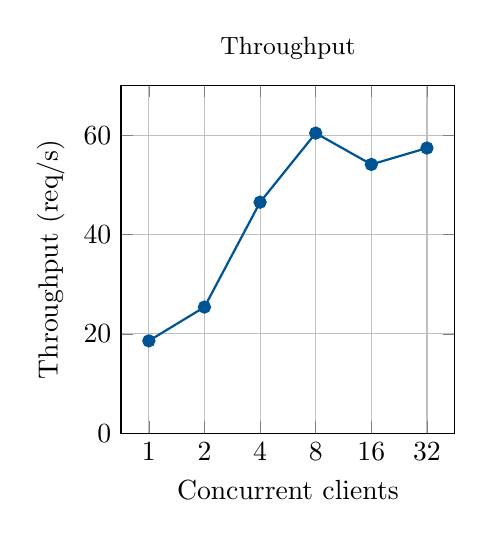
\begin{tikzpicture}
\begin{axis}[width=0.48\textwidth,height=6cm,xmode=log,log basis x=2,xtick={1,2,4,8,16,32},
  xticklabels={1,2,4,8,16,32},xlabel={Concurrent clients},ylabel={Throughput (req/s)},
  ymin=0,ymax=70,grid=major,title={\small Throughput}]
\addplot[thick,mark=*,color=spitblue] coordinates {(1,18.6)(2,25.4)(4,46.5)(8,60.4)(16,54.1)(32,57.4)};
\end{axis}
\end{tikzpicture}\hfill
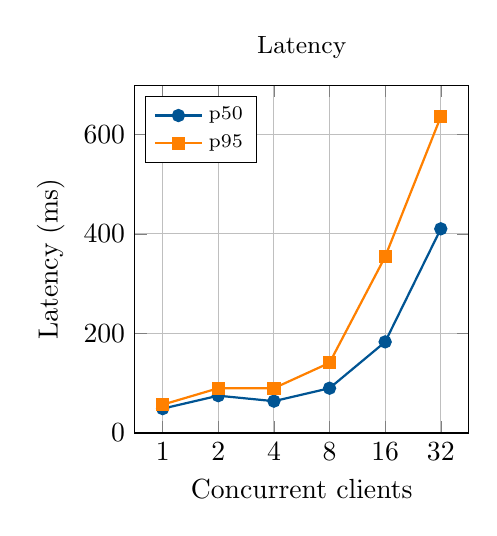
\begin{tikzpicture}
\begin{axis}[width=0.48\textwidth,height=6cm,xmode=log,log basis x=2,xtick={1,2,4,8,16,32},
  xticklabels={1,2,4,8,16,32},xlabel={Concurrent clients},ylabel={Latency (ms)},
  ymin=0,grid=major,legend pos=north west,legend style={font=\scriptsize},title={\small Latency}]
\addplot[thick,mark=*,color=spitblue] coordinates {(1,49)(2,75)(4,64)(8,90)(16,183)(32,410)};
\addplot[thick,mark=square*,color=orange] coordinates {(1,57)(2,90)(4,90)(8,141)(16,354)(32,635)};
\legend{p50,p95}
\end{axis}
\end{tikzpicture}
\caption{Throughput and latency under increasing concurrent load (measured)}
\label{fig:load}
\end{figure}

\begin{table}[H]
\centering
\caption{Extraction performance on the real 10-page PDF (median of 5 runs)}
\label{tab:extractperf}
\small
\begin{tabular}{@{}lr@{}}
\toprule
\textbf{Metric} & \textbf{Value}\\
\midrule
Pages / rows produced & 10 / 570 (453 classes)\\
Extraction time, whole pipeline & 1.65 s (runs: 1.72, 1.65, 1.64, 1.69, 1.64 s)\\
Per page & $\approx$0.17 s\\
Peak memory & 82 MB\\
\bottomrule
\end{tabular}
\end{table}

\subsection{Bottleneck Identification}
\begin{enumerate}
\item \textbf{CPU of the API processes.} Throughput stops growing at about 55--60 req/s from 8 clients
      while CPU reaches 60--76\%, and the rest of the CPU is taken by PostgreSQL and the load generator
      on the same machine. Beyond that point extra clients only add queueing delay, so p50 rises
      roughly linearly with $N$.
\item \textbf{Per-request work:} each search resolves the context, loads the vocabulary of the
      timetable (about 200 labels) and runs one or two templates. Vocabulary loading is the largest
      repeated cost.
\item \textbf{Database round trips:} before optimisation a search issued about 50 SQL statements
      because related rows were loaded lazily (N+1 problem).
\end{enumerate}

\subsection{Optimisation and Improvement}
\begin{table}[H]
\centering
\caption{Optimisations performed (before/after)}
\label{tab:optim}
\small
\begin{tabularx}{\textwidth}{@{}p{4cm}p{3.2cm}p{3.2cm}X@{}}
\toprule
\textbf{Change} & \textbf{Before} & \textbf{After} & \textbf{Effect}\\
\midrule
Eager loading of course/staff/room/batch (N+1 fix) & $\approx$50 SQL statements / search & $\approx$25 & Halved round trips; latency now 37--47~ms\\
Batched vocabulary loading & 1 query per label & 1 query per entity type & Constant number of queries per search\\
Composite indexes led by \texttt{timetable\_id} & -- & index range scans & ``Now/next'' independent of other timetables' size\\
Intended-overlap rules in conflict detection & 542 reported overlaps & 2 & Removes false alarms (quality, not speed)\\
Extraction moved to background worker & -- & API never blocked by OCR & Search latency unaffected by uploads\\
\bottomrule
\end{tabularx}
\end{table}
Further options: cache the vocabulary per (timetable, \texttt{data\_version}); add more API processes
or machines (horizontal scaling); use a shared rate-limit store (Redis/PostgreSQL) for several machines.

\subsection{Cloud Deployment and Resource Utilisation}
\begin{itemize}
\item \textbf{Architecture:} Figure~\ref{fig:deploy}. One Render \emph{free} web service runs a Docker
      image (multi-stage build: Node builds the web app, then a Python image with Tesseract runs
      FastAPI, the worker thread and the static web app), plus a free managed PostgreSQL database.
\item \textbf{Configuration:} \texttt{render.yaml} (blueprint); the secret key is generated by Render,
      \texttt{DEMO\_PASSWORD} is entered at deploy time, production mode refuses the published
      development password, and demo data is seeded only into an empty database.
\item \textbf{Resources:} free instance with 512~MB RAM and a shared fraction of a CPU. Measured
      memory of one API process ($\approx$115~MB) plus extraction peak ($\approx$82~MB) fits within it.
\item \textbf{Limits:} the service sleeps after 15 minutes idle (first request then takes about a
      minute); the free database expires after 30 days; 750 free instance hours per month~\cite{render}.
\item \textbf{Scaling approach (projected):} a paid always-on instance with 2+ API processes and a
      separate worker; managed PostgreSQL with backups; horizontal scaling behind the platform's load
      balancer, because the API is stateless.
\end{itemize}

\subsection{Scalability Limitations}
\begin{itemize}
\item \textbf{Maximum tested workload:} 32 concurrent closed-loop clients (960 requests) with 0 wrong
      answers and 57 req/s, on a 4-core development VM shared with the database and the load generator.
\item \textbf{Projection (not tested):} with think time of about 10~s between requests, 57 req/s
      corresponds to several hundred simultaneously active users on similar hardware. This is an
      estimate only; a real capacity test must run on the deployment hardware.
\item The free cloud tier is much smaller (shared CPU); it is suitable for a demo, not for the whole college.
\item The rate limiter is per process. With several machines it must move to a shared store.
\item OCR of large scanned PDFs is CPU-heavy; with many simultaneous uploads more workers are needed.
\end{itemize}

\newpage

\section{Testing and Validation}

\subsection{Testing Strategy}
Testing followed the test pyramid: many fast unit tests, fewer integration tests, and a small number
of end-to-end tests that drive the real user interface. Tests were written alongside each module and
the full suite was run before every commit. The real college PDF is part of the test fixtures, so
every change to the parser is checked against the real document (regression testing).

\begin{table}[H]
\centering
\caption{Test suites and results (latest run)}
\label{tab:suites}
\small
\begin{tabularx}{\textwidth}{@{}p{4.5cm}p{1.8cm}X@{}}
\toprule
\textbf{Suite (file)} & \textbf{Tests} & \textbf{What it covers}\\
\midrule
\texttt{test\_\allowbreak{}auth.py} & 15 & Login, tokens, rotation, reuse detection, suspension, role change, rate limit, reset-code safety\\
\texttt{test\_\allowbreak{}extraction.py} & 24 & PDF-01\ldots PDF-13 of the extraction specification, OCR, other formats, time rules, cell grammar\\
\texttt{test\_\allowbreak{}reference\_\allowbreak{}pdf.py} & 14 & Regression on the real college PDF (10 pages)\\
\texttt{test\_\allowbreak{}college\_\allowbreak{}seed.py} & 22 & Real PDF end to end: seed $\rightarrow$ API as student, professor, HOD, Admin; 7 composed query-plan tests (count, first/last, busiest day, lab filter scope, exists, counting professors/subjects, clarification, injection)\\
\texttt{test\_\allowbreak{}uploads\_\allowbreak{}and\_\allowbreak{}domains.py} & 13 & Upload $\rightarrow$ worker $\rightarrow$ status, primary rules, IDOR, idempotency, corrections\\
\texttt{test\_\allowbreak{}query\_\allowbreak{}engine.py} & 59 & Every specialised operation Q01--Q30, composed plans in the personal domain, clarifications, domain isolation, injection text\\
\texttt{test\_\allowbreak{}academics\_\allowbreak{}admin.py} & 13 & Registration, promotion, concurrency, master data, role matrix, conflicts\\
\texttt{test\_\allowbreak{}deploy.py} & 8 & Web app serving, \texttt{HEAD} connectivity check, production safety\\
\midrule
\textbf{Back end (pytest)} & \textbf{168} & \textbf{168 passed, 0 failed}\\
Mobile unit/component (Jest) & 20 & API client, single-flight refresh, offline cache, result renderer (incl.\ count and day-summary cards), status labels\\
End-to-end (Playwright) & 24 + 21 & Real college timetable flow 24/24 (incl.\ composed questions); synthetic smoke flow incl.\ upload 21/21\\
TypeScript \texttt{strict} type check & -- & clean\\
\bottomrule
\end{tabularx}
\end{table}

\subsection{Unit Testing}
Unit tests check individual functions with exact inputs and outputs. Examples:
\texttt{test\_\allowbreak{}time\_\allowbreak{}rules} (time-label parsing and sequence resolution, including ``12.15 a.m.\ to
01.15 p.m.''), \texttt{test\_cell\_grammar\_explicit\_time\_and\_electives} (cell parser),
\texttt{test\_\allowbreak{}signature\_\allowbreak{}detection\_\allowbreak{}rejects\_\allowbreak{}mismatch} (plain text named \texttt{x.pdf} is rejected; a real PDF is recognised even when renamed),
and, in Jest, the single-flight token refresh (three concurrent 401 responses produce exactly one
refresh call).

\subsection{Integration Testing}
Integration tests use a real PostgreSQL test database and FastAPI's test client:
\texttt{test\_\allowbreak{}personal\_\allowbreak{}upload\_\allowbreak{}processing\_\allowbreak{}and\_\allowbreak{}primary\_\allowbreak{}unchanged} uploads a file, runs the worker and
checks the status transitions; \texttt{test\_real\_pdf\_end\_to\_end\_upload\_persist\_activate} runs the
real PDF through upload, worker, database and activation; \texttt{test\_college\_seed.py} loads the real
timetable and asks questions as different roles. Playwright then tests the front end, back end and
database together in a browser.

\subsection{Functional Testing}
Each functional requirement has at least one test (Table~\ref{tab:testcases}). The intent tests are
organised one per intent (\texttt{test\_q01\_\ldots} to \texttt{test\_q30\_\ldots}), each with valid and
negative paths.

\subsection{Non-Functional Testing}
\begin{itemize}
\item \textbf{Performance:} single-user latency and load tests (Chapter~8).
\item \textbf{Security:} role escalation (\texttt{test\_role\_escalation\_not\_possible\_via\_client}),
      IDOR (\texttt{test\_idor\_other\_users\_personal\_timetable}), SQL-injection text
      (\texttt{test\_sql\_injection\_text\_is\_data}), raw SQL parameters rejected, rate limiting,
      token reuse detection, reset codes never logged in production. A manual security audit (OWASP
      categories) found one critical issue (P0-1), which was fixed and verified with 9 checks.
\item \textbf{Reliability:} worker retry, crash recovery by heartbeat, idempotent uploads.
\item \textbf{Usability:} the app was tried on Android and iPhone (Expo Go) and laptop browsers by the
      team. This hands-on use led to hiding Admin review notices from students and fixing the
      archive banner.
\item \textbf{Portability:} Android and iOS bundles compile; the web build runs in Chrome; the Docker
      image deploys on Render.
\end{itemize}

\subsection{Boundary and Invalid-Input Testing}
\begin{itemize}
\item Empty, corrupt and wrong-type files; a PDF with no table; a 0-entry result (\textsc{Unusable}).
\item Time boundaries: back-to-back classes (9--10 and 10--11) do \emph{not} conflict (end-exclusive);
      a class at exactly its start time is ``current''.
\item Ambiguous inputs: ``Am I free at 2?'' (a.m./p.m.), ``5/6'' (date order), an unknown professor
      name, a misspelled name (suggestions only).
\item Date range larger than 31 days rejected; unknown parameters and raw SQL rejected.
\item Invalid state transitions: an \textsc{Unusable} or \textsc{Failed} timetable cannot become
      primary; a student cannot be promoted twice; an Admin cannot remove their own Admin role.
\item Missing configuration: no lunch boundary, no working hours, no week start $\rightarrow$
      clarification or explicit ``not configured'', never an assumed value.
\end{itemize}

\subsection{Concurrency and Stress Testing}
\begin{itemize}
\item \texttt{test\_concurrent\_activation\_single\_default}: two threads activate different timetables
      at the same time; exactly one default results, with no lost update.
\item \texttt{test\_concurrent\_promotions\_cannot\_create\_two\_open\_placements}: simultaneous
      promotions of the same student; the partial unique index and row locks guarantee one open placement.
\item Single-flight refresh under concurrent 401s (Jest).
\item Load test up to 32 concurrent clients: 960 requests, 0 wrong answers, no deadlocks or errors
      (Section~8.7).
\end{itemize}

\subsection{Test Case Specification}
\begingroup\footnotesize
\setlength{\tabcolsep}{3pt}
\begin{longtable}{@{}p{1.15cm}p{1.2cm}>{\raggedright\arraybackslash}p{4.4cm}>{\raggedright\arraybackslash}p{3.6cm}>{\raggedright\arraybackslash}p{2.1cm}p{0.6cm}>{\raggedright\arraybackslash}p{2.3cm}@{}}
\caption{Test case specification}\label{tab:testcases}\\
\toprule
\textbf{TC} & \textbf{Req.} & \textbf{Scenario (input)} & \textbf{Expected result} & \textbf{Actual} & \textbf{P/F} & \textbf{Evidence}\\
\midrule
\endfirsthead
\toprule
\textbf{TC} & \textbf{Req.} & \textbf{Scenario (input)} & \textbf{Expected result} & \textbf{Actual} & \textbf{P/F} & \textbf{Evidence}\\
\midrule
\endhead
TC-01 & FR-01 & Wrong password vs unknown user (Two bad logins) & Same generic error & As expected & P & test\_\allowbreak{}auth\\
TC-02 & FR-01 & Refresh-token reuse (Reuse rotated token) & Whole family revoked, 401 & As expected & P & test\_\allowbreak{}auth\\
TC-03 & FR-02 & Role escalation (Student sends \texttt{roles:[ADMIN]}) & Ignored; admin APIs 403 & As expected & P & test\_\allowbreak{}auth\\
TC-04 & FR-03 & Wrong file type (Text file named \texttt{.pdf}) & Rejected, nothing stored & As expected & P & test\_\allowbreak{}extraction\\
TC-05 & FR-03 & Upload does not change primary (Upload new file) & Primary unchanged & As expected & P & test\_\allowbreak{}uploads\\
TC-06 & FR-03 & Retry same upload (Same client\_\allowbreak{}request\_\allowbreak{}id twice) & One archive record & As expected & P & test\_\allowbreak{}uploads\\
TC-07 & FR-04 & Real PDF extraction (10-page college PDF) & $\geq$95\% verified & 452/453 (99.8\%) & P & test\_\allowbreak{}college\_\allowbreak{}seed\\
TC-08 & FR-04 & Stacked lab cell (Cell with A1--A4) & 4 entries, own room/teacher & As expected & P & test\_\allowbreak{}reference\_\allowbreak{}pdf\\
TC-09 & FR-04 & Noon row typo (``12.15 a.m.\ to 01.15 p.m.'') & 12:15--13:15 with visible note & As expected & P & test\_\allowbreak{}reference\_\allowbreak{}pdf\\
TC-10 & FR-04 & Scanned PDF (Image-only PDF) & OCR, entries \textsc{Unverified} & As expected & P & test\_\allowbreak{}extraction\\
TC-11 & FR-05 & No-table PDF (Plain text PDF) & \textsc{Unusable}, cannot be primary & As expected & P & test\_\allowbreak{}extraction\\
TC-12 & FR-06 & Correction audited (Admin edits room) & Original kept, audit row & As expected & P & test\_\allowbreak{}uploads\\
TC-13 & FR-07 & Concurrent activation (2 threads activate) & Exactly one default & As expected & P & test\_\allowbreak{}academics\\
TC-14 & FR-09 & Dashboard = query (Home vs ``next class?'') & Identical entry & As expected & P & test\_\allowbreak{}query\_\allowbreak{}engine\\
TC-15 & FR-10 & Lab group isolation (SE-A1, Wednesday) & Only A1 labs & As expected & P & test\_\allowbreak{}college\_\allowbreak{}seed\\
TC-16 & FR-11 & Lunch per year (SE vs TE ``after lunch'') & 14:15 vs 13:15 from PDF & As expected & P & test\_\allowbreak{}college\_\allowbreak{}seed\\
TC-17 & FR-11 & Ambiguous time (``Am I free at 2?'') & Clarification a.m./p.m. & As expected & P & test\_\allowbreak{}query\_\allowbreak{}engine, e2e\\
TC-18 & FR-11 & Injection text (``'; DROP TABLE \ldots'') & Treated as text; no SQL run & As expected & P & test\_\allowbreak{}query\_\allowbreak{}engine\\
TC-19 & FR-11 & Cross-domain compare (Q30 question) & UNSUPPORTED, no query executed & As expected & P & test\_\allowbreak{}query\_\allowbreak{}engine\\
TC-20 & FR-12 & Free rooms on a floor (``free rooms on floor 5 at 10'') & Rooms without overlapping class & As expected & P & test\_\allowbreak{}query\_\allowbreak{}engine\\
TC-21 & FR-13 & Clashes in real PDF (Real timetable) & Exactly 2 genuine clashes & 2 (SP Fri; 603-2 Tue) & P & test\_\allowbreak{}college\_\allowbreak{}seed\\
TC-22 & FR-14 & IDOR personal (Other user's timetable id) & 404 + audit & As expected & P & test\_\allowbreak{}uploads\\
TC-23 & FR-15 & Promotion (Preview + confirm) & History kept, new batch & As expected & P & test\_\allowbreak{}academics\\
TC-24 & FR-15 & Concurrent promotion (2 threads) & One open placement & As expected & P & test\_\allowbreak{}academics\\
TC-25 & FR-17 & Student without batch (``next class?'') & Setup-required message & As expected & P & test\_\allowbreak{}college\_\allowbreak{}seed\\
TC-26 & NFR-04 & Reset code in prod (Production, no SMTP) & Code never in response/log & As expected & P & test\_\allowbreak{}deploy\\
TC-27 & NFR-03 & Connectivity probe (\texttt{HEAD /}) & 200 (not 405) & As expected & P & test\_\allowbreak{}deploy\\
TC-28 & NFR-01 & Search latency (50 req/intent) & p50 $<$ 300 ms & 37--47 ms & P & Table~\ref{tab:latency}\\
TC-29 & NFR-03 & Load (32 clients, 960 req) & 0 wrong answers & 0 & P & Table~\ref{tab:loadresults}\\
TC-30 & UI & Full student/HOD flow (Browser, real data) & All steps pass & 24/24 & P & college.e2e.mjs\\
TC-31 & FR-11 & Count with filters (``How many labs do I have this week?'') & Count = distinct lab periods; only labs & As expected & P & test\_\allowbreak{}college\_\allowbreak{}seed\\
TC-32 & FR-11 & First/last (``When is my last class on Friday?'') & Same as max end of the Friday listing & As expected & P & test\_\allowbreak{}college\_\allowbreak{}seed\\
TC-33 & FR-11 & Day-wise ordering (``Which day is my busiest / finish earliest?'') & Days sorted by classes / finish time & As expected & P & test\_\allowbreak{}college\_\allowbreak{}seed\\
TC-34 & FR-02 & Composed plan keeps role scope (``Show my labs'', ``Show SE-B labs'') & Only own lab group; no other batch & As expected & P & test\_\allowbreak{}college\_\allowbreak{}seed\\
\bottomrule
\end{longtable}
\endgroup

\subsection{Defect Identification and Resolution}
\begin{table}[H]
\centering
\caption{Significant defects found, fixed and re-tested}
\label{tab:defects}
\small
\begin{tabularx}{\textwidth}{@{}p{1cm}p{4cm}Xp{2.3cm}@{}}
\toprule
\textbf{ID} & \textbf{Defect} & \textbf{Root cause and fix} & \textbf{Re-test}\\
\midrule
D-1 & 542 ``conflicts'' in real PDF & Parallel labs/electives treated as clashes; added intended-overlap rules & 2 remain; test asserts exact set\\
D-2 & Noon classes missing & ``12.15 a.m.'' rejected as invalid; added neighbour-proof rule & Regression test\\
D-3 & Unknown legend codes shown as errors & Codes not in legend are valid; downgraded to INFO & Test\\
D-4 & Students saw ``needs review'' warnings & Admin-only notice leaked to students; filtered by role & Test + screenshot\\
D-5 & Archive banner shown when choosing the official timetable & Explicit selection of primary treated as archive & Test\\
D-6 & Web app stuck on ``Loading\ldots'' & \texttt{HEAD /} returned 405 $\Rightarrow$ ``offline''; allow HEAD & Test + e2e\\
D-7 & Account takeover via reset (P0-1) & Reset code exposed outside development; never returned/logged in production & 9 checks + test\\
D-8 & $\approx$50 SQL statements per search & N+1 lazy loading; eager loading & $\approx$25; latency measured\\
D-9 & App incompatible with Expo Go on iPhone & SDK 57 vs required 58; upgraded, fixed types and Jest mocks & All tests + e2e\\
\bottomrule
\end{tabularx}
\end{table}

\subsection{Validation Against KPIs}
\begin{table}[H]
\centering
\caption{KPI targets (Chapter 1) vs measured results}
\label{tab:kpivalid}
\small
\begin{tabularx}{\textwidth}{@{}p{3.6cm}p{2.6cm}Xp{1.4cm}@{}}
\toprule
\textbf{KPI} & \textbf{Target} & \textbf{Measured} & \textbf{Met?}\\
\midrule
Extraction verification rate & $\geq$95\% & 452/453 = 99.8\% (remaining entry has no time in the PDF) & Yes\\
False clash reports & 0 & 0 (2 reported, both genuine) & Yes\\
Response time (median, 1 user) & $<$300 ms & 37--47 ms & Yes\\
Throughput (4 workers) & $\geq$30 req/s & 46.5 req/s at 4 clients, 60.4 at 8 & Yes\\
Reliability under concurrency & 100\% & 960/960 correct at 32 clients & Yes\\
Functional correctness & 100\% tests pass & 168/168, 20/20, 24/24, 21/21 & Yes\\
Extraction time (10 pages) & $<$10 s & 1.65 s & Yes\\
Memory per API worker; DB size & $<$300 MB; $<$50 MB & $\approx$115 MB; 12 MB & Yes\\
Supported question types & $\geq$25 & 30 specialised operations + composed plans (8 operations $\times$ filters $\times$ windows) & Yes\\
\bottomrule
\end{tabularx}
\end{table}

\subsection{Limitations and Untested Scenarios}
\begin{itemize}
\item \textbf{Extraction accuracy} has not been measured against a hand-labelled ground truth
      (precision/recall). The 99.8\% figure is the share of entries the system \emph{verified itself};
      the 2 clashes were confirmed by hand.
\item \textbf{Capacity on production hardware} has not been tested; the load test ran on a development VM.
\item \textbf{Push notifications} (need a store build), \textbf{SMTP e-mail} and \textbf{store builds}
      (APK/TestFlight) have not been exercised.
\item \textbf{Device matrix:} tried on a few phones through Expo Go and the web; no systematic
      small-screen/large-text/accessibility audit.
\item \textbf{Other colleges' timetable layouts} have not been tested; only our department's PDF and
      synthetic fixtures.
\item \textbf{Long-running operation} (database expiry, backups, multi-semester data) has not been
      tested beyond the 30-day free-tier window.
\end{itemize}

\newpage

\section{Results, Demonstration and Discussion}

\subsection{Implemented Features}
\begin{table}[H]
\centering
\caption{Implementation status of features (implemented = code + automated test)}
\label{tab:features}
\small
\begin{tabularx}{\textwidth}{@{}Xp{2.4cm}p{3.3cm}@{}}
\toprule
\textbf{Feature} & \textbf{Status} & \textbf{Evidence}\\
\midrule
Login, activation, password reset, 5 roles with server-side RBAC & Implemented, tested & test\_auth (15)\\
Upload PDF / scanned PDF / image / XLSX / XLS / CSV / DOCX / DOC & Implemented, tested & test\_extraction (24)\\
Extraction tuned on real college PDF (labs, legends, noon row, BE combined, LLC) & Implemented, tested & test\_reference\_pdf (14)\\
Validation, review \& correction (audited), activation, archives & Implemented, tested & test\_uploads (13)\\
Conflict detection (professor / room / batch) & Implemented, tested & 2 genuine clashes found\\
Role dashboards, weekly view, class details & Implemented, e2e tested & Figures \ref{fig:screens1}--\ref{fig:screens2}\\
Natural-language search: compositional query plans (count, first/last, per day, lab/lecture, before/after) plus specialised operations, clarifications & Implemented, tested & test\_query\_engine (59), composed tests (7)\\
Personal timetables, strictly separate & Implemented, tested & domain tests\\
Promotion, fresher registration, master data, users, audit log & Implemented, tested & test\_academics (13)\\
Android, iPhone (Expo Go), laptop browser & Implemented; web e2e; device tried & Screenshots\\
Free online demo (Render) & Deployed & \texttt{render.yaml}, demo link\\
Push notifications & Implemented, not verified & Needs store build\\
E-mail delivery (SMTP) & Implemented, not verified & No mail server configured\\
Installable store apps (APK/TestFlight) & Configured (EAS), not built & --\\
\bottomrule
\end{tabularx}
\end{table}

\subsection{Screenshots and Demonstration Evidence}
The screenshots below were captured automatically by the Playwright end-to-end tests running the real
app (web build, phone-sized viewport) against the real API, with the college's timetable loaded.

\begin{figure}[H]
\centering
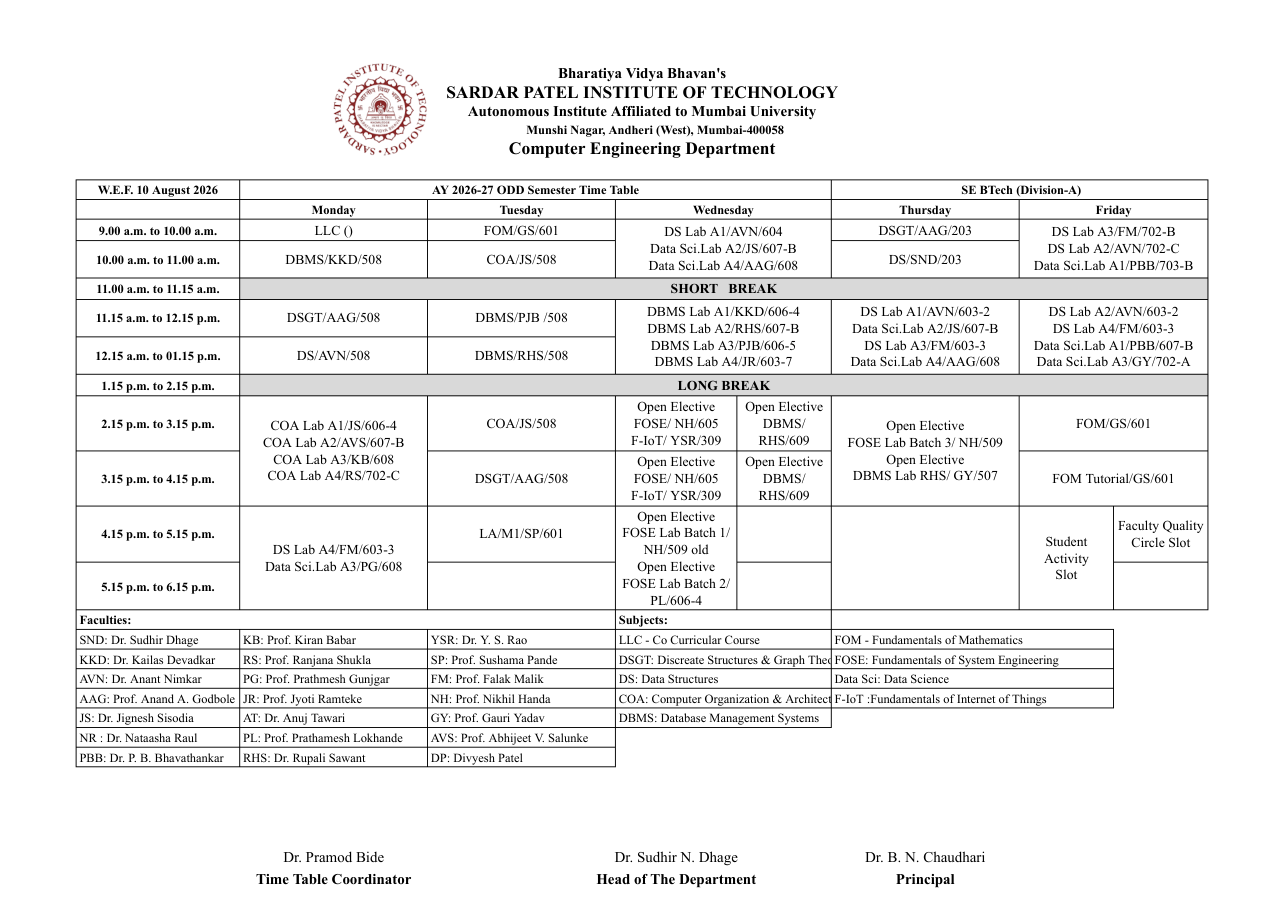
\includegraphics[width=0.75\textwidth]{figures/real-pdf-page1.png}
\caption{Input: page 1 of the college's real timetable PDF (S.E.\ Division A), with stacked lab cells and legend}
\label{fig:realpdf}
\end{figure}

\begin{figure}[H]
\centering
\begin{subfigure}[t]{0.24\textwidth}\centering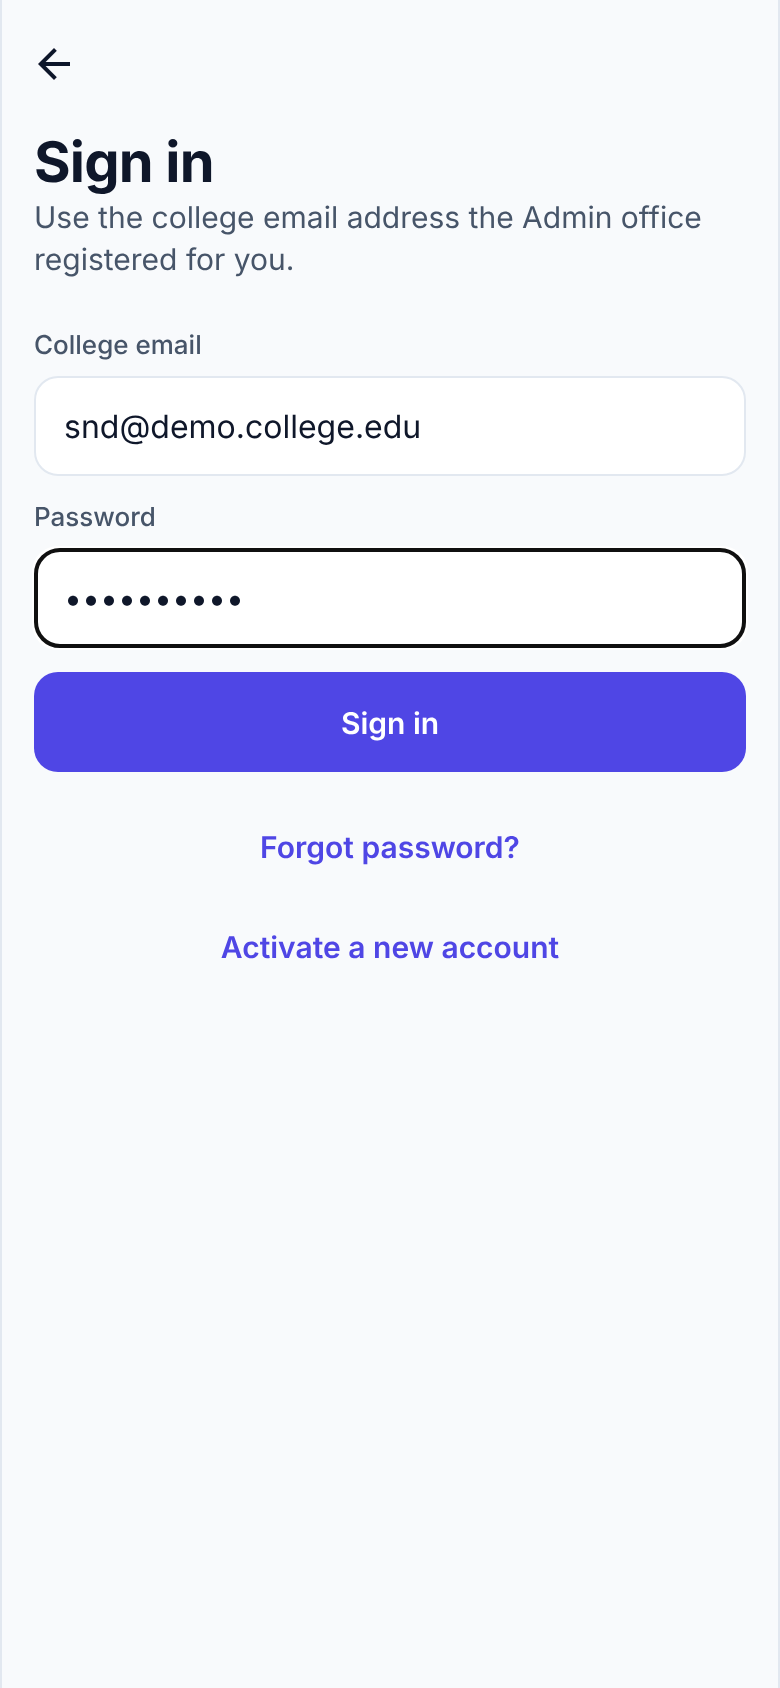
\includegraphics[width=\linewidth]{figures/screens/login.png}\caption{Sign in}\end{subfigure}\hfill
\begin{subfigure}[t]{0.24\textwidth}\centering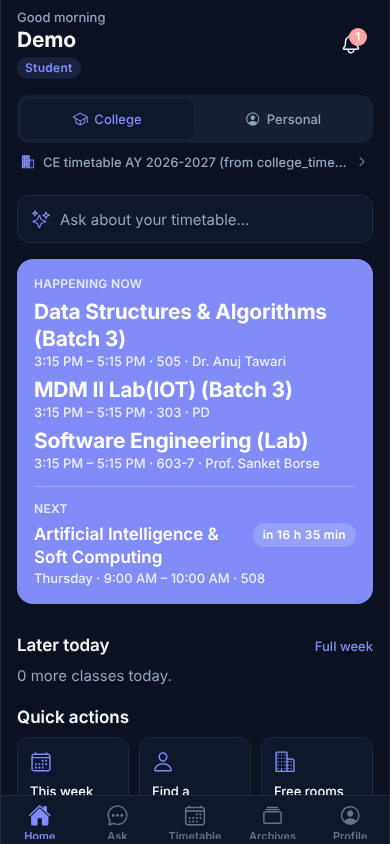
\includegraphics[width=\linewidth]{figures/screens/home-dark.png}\caption{Student home (dark mode): now / next}\end{subfigure}\hfill
\begin{subfigure}[t]{0.24\textwidth}\centering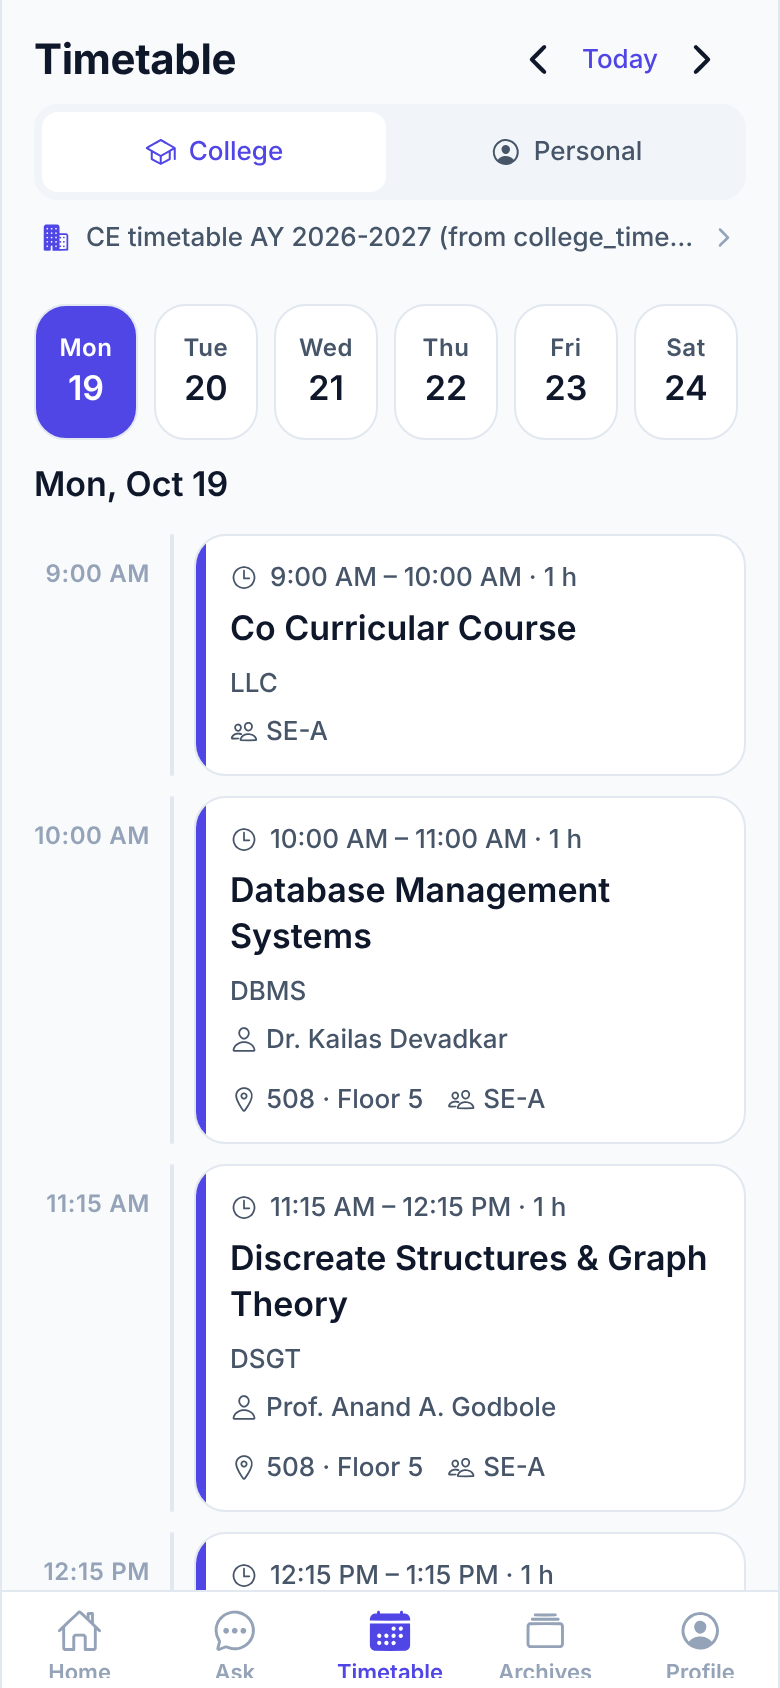
\includegraphics[width=\linewidth]{figures/screens/student-monday.png}\caption{Week view, Monday (SE-A1)}\end{subfigure}\hfill
\begin{subfigure}[t]{0.24\textwidth}\centering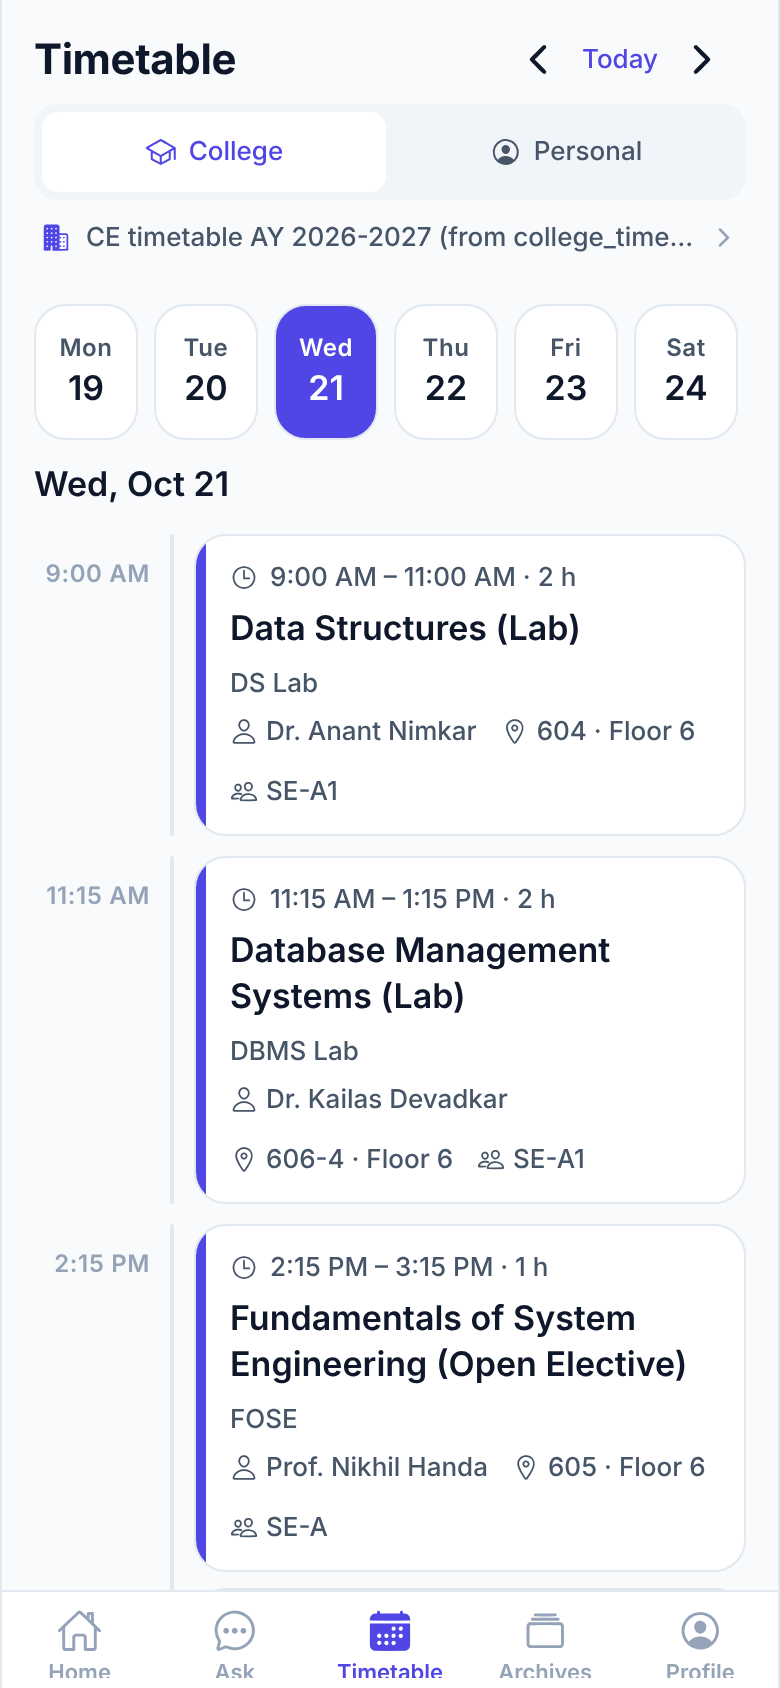
\includegraphics[width=\linewidth]{figures/screens/student-wednesday-lab.png}\caption{Only lab group A1's labs}\end{subfigure}
\caption{Student screens}
\label{fig:screens1}
\end{figure}

\begin{figure}[H]
\centering
\begin{subfigure}[t]{0.24\textwidth}\centering
\includegraphics[width=\linewidth]{figures/screens/class-details.png}\caption{Class details with source page and raw text (LLC: no teacher/room)}\end{subfigure}\hfill
\begin{subfigure}[t]{0.24\textwidth}\centering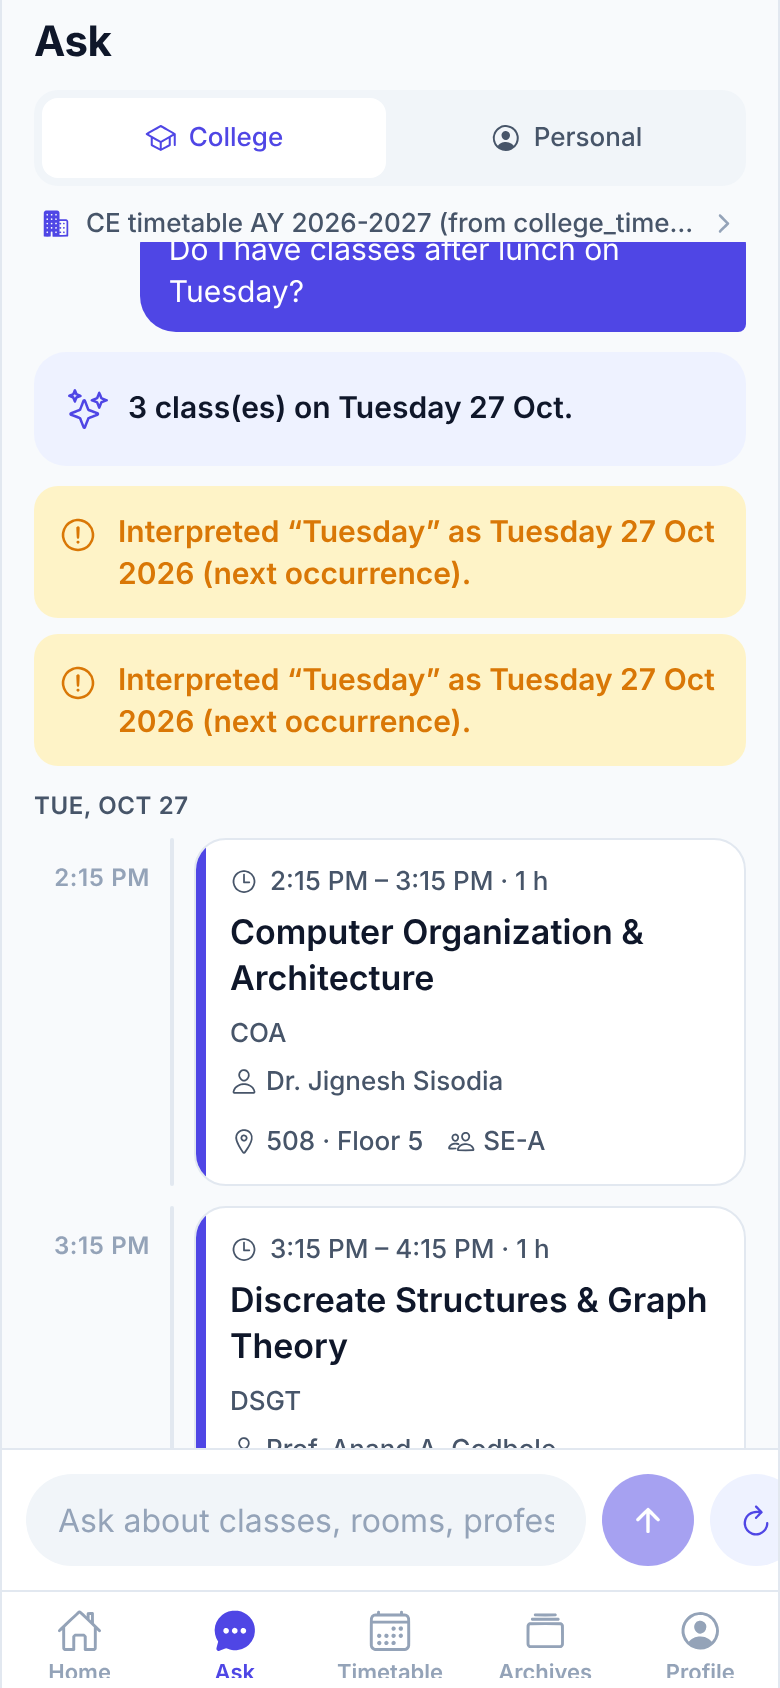
\includegraphics[width=\linewidth]{figures/screens/ask-after-lunch.png}\caption{``Classes after lunch on Tuesday?'' uses SE lunch}\end{subfigure}\hfill
\begin{subfigure}[t]{0.24\textwidth}\centering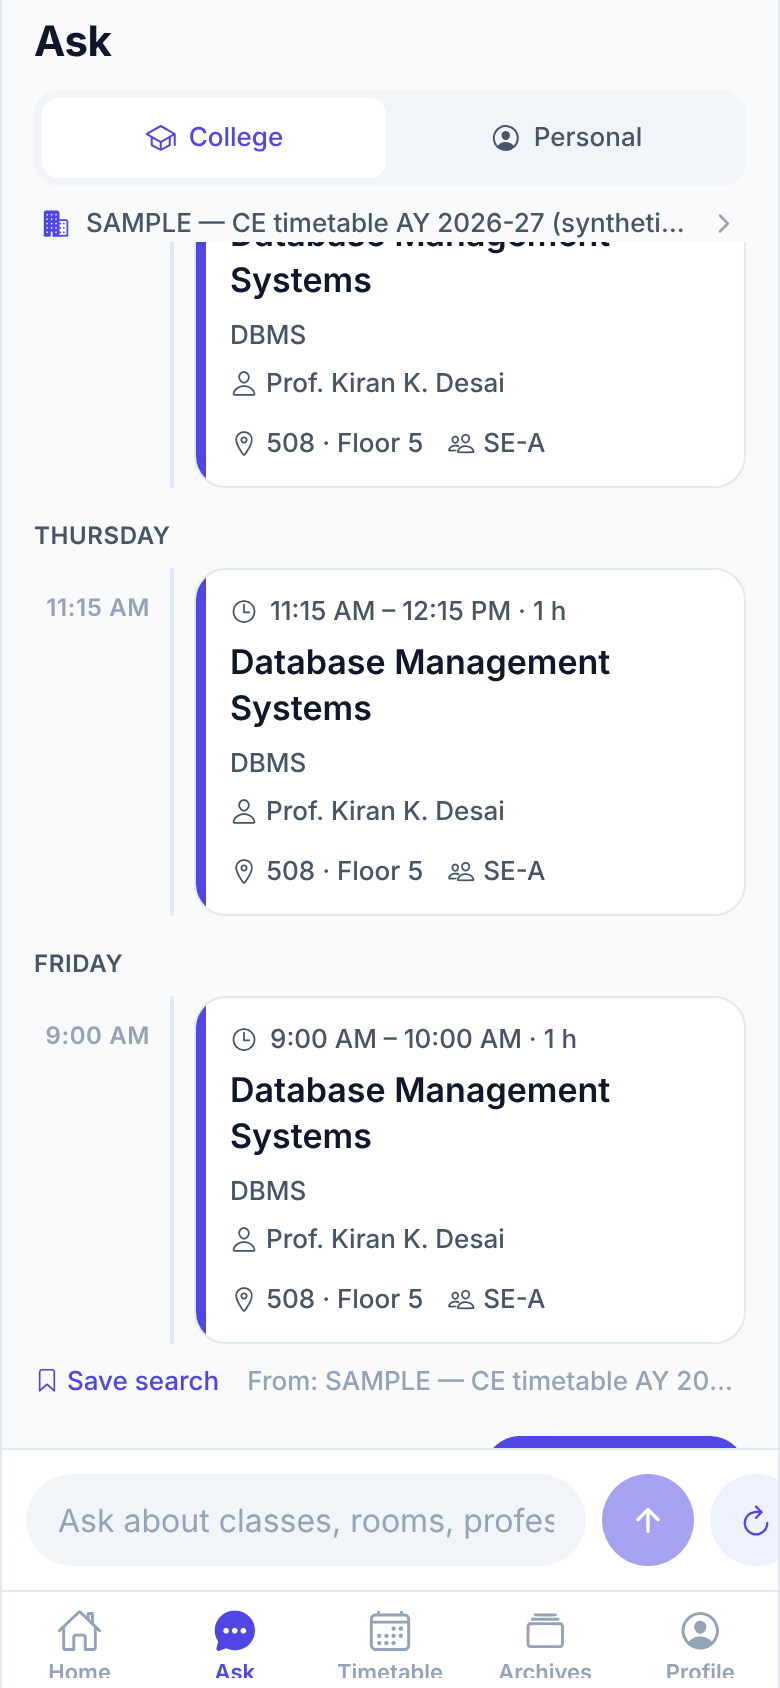
\includegraphics[width=\linewidth]{figures/screens/clarify-ampm.png}\caption{``Am I free at 2?'' asks a.m.\ or p.m.}\end{subfigure}\hfill
\begin{subfigure}[t]{0.24\textwidth}\centering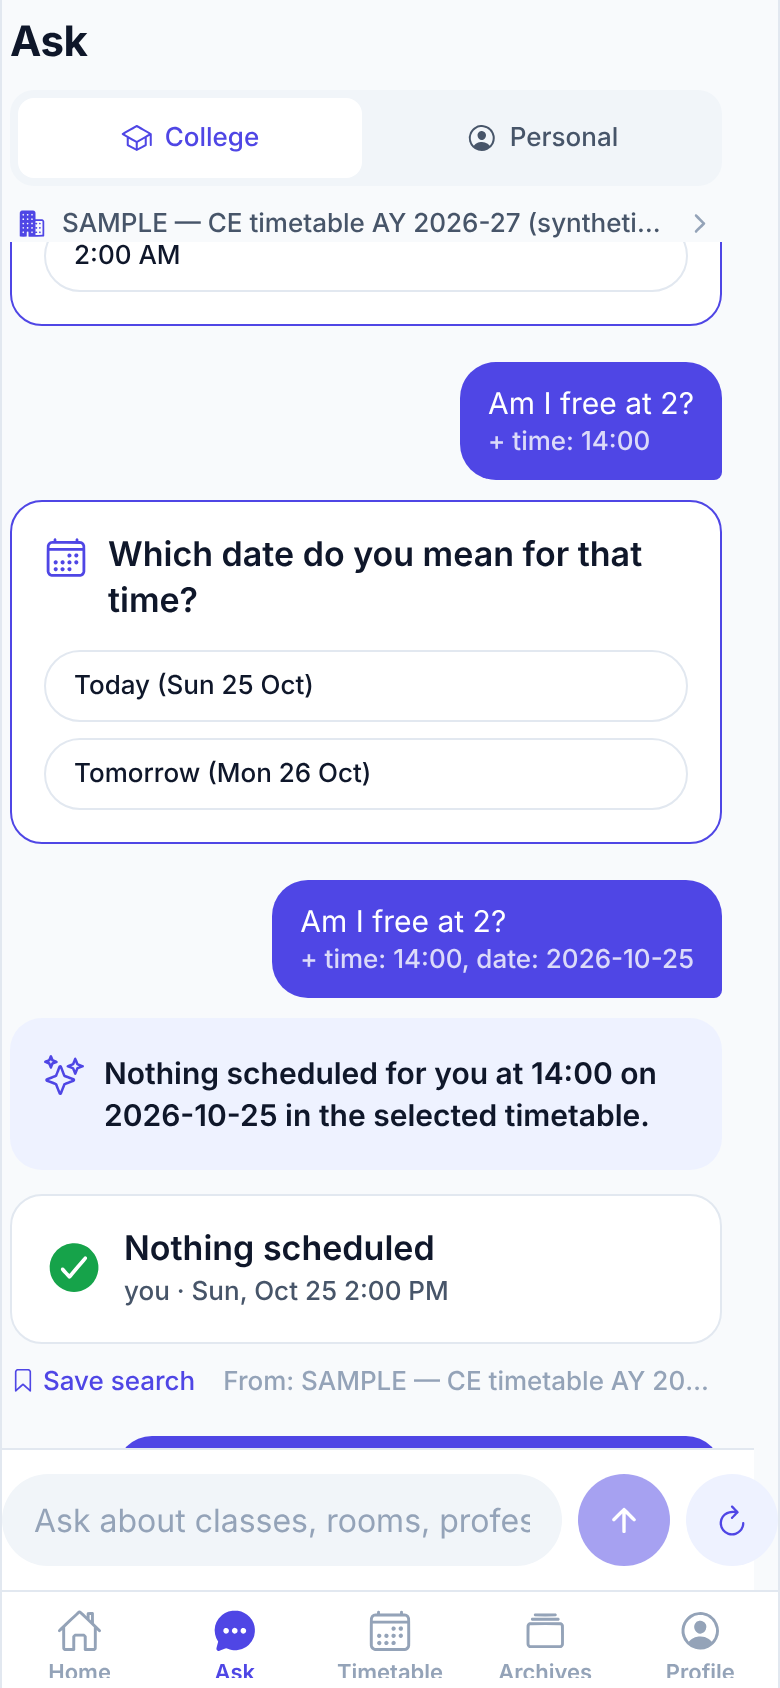
\includegraphics[width=\linewidth]{figures/screens/cross-domain.png}\caption{After choosing 2 PM and the date: answer}\end{subfigure}
\caption{Natural-language search (Ask tab)}
\label{fig:screensask}
\end{figure}

\begin{figure}[H]
\centering
\begin{subfigure}[t]{0.24\textwidth}\centering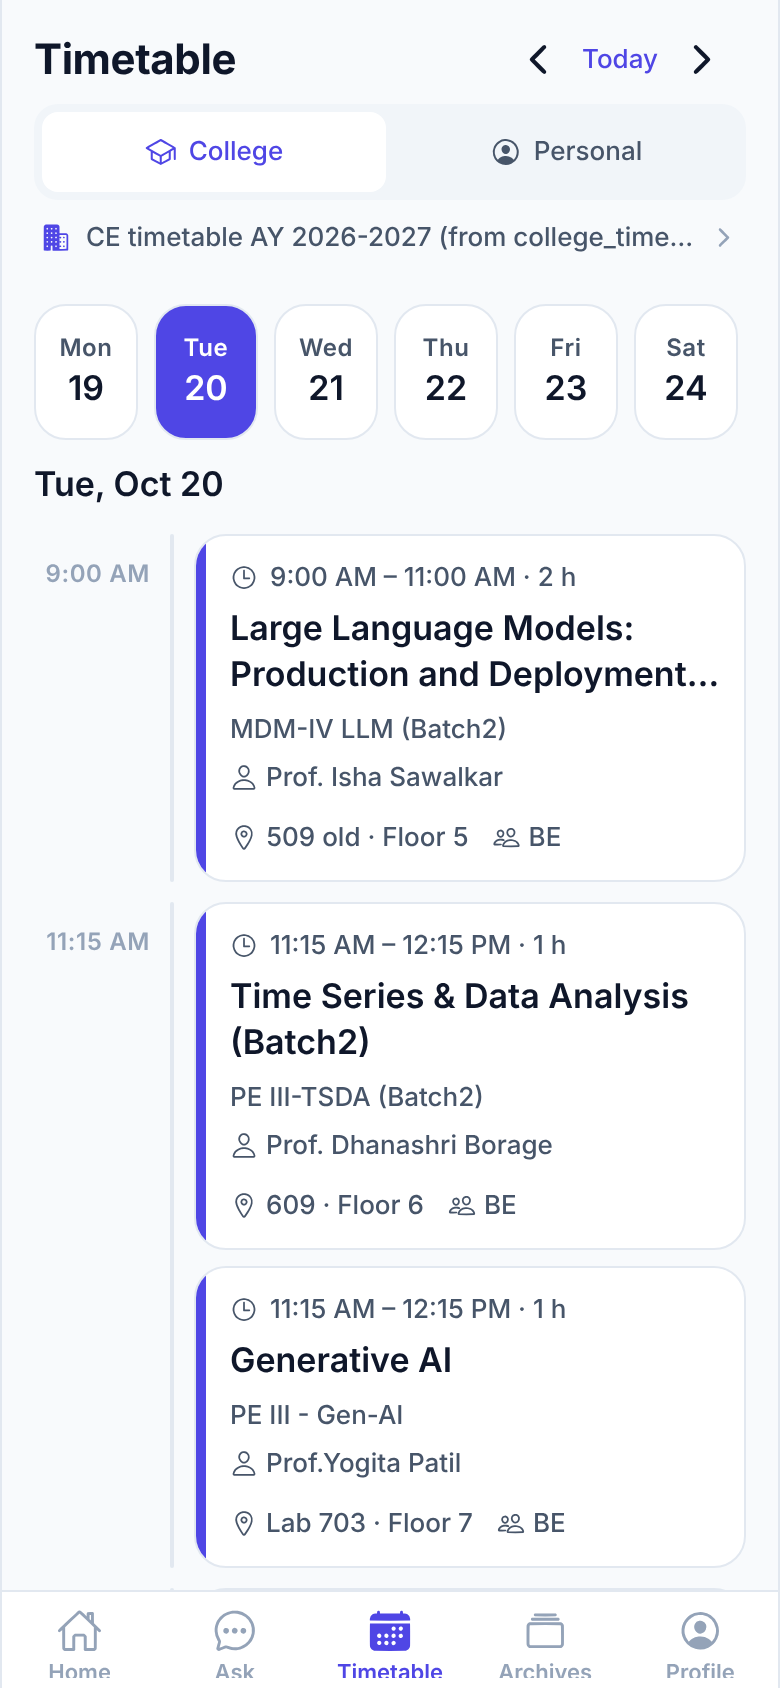
\includegraphics[width=\linewidth]{figures/screens/be-combined.png}\caption{B.E.\ combined electives}\end{subfigure}\hfill
\begin{subfigure}[t]{0.24\textwidth}\centering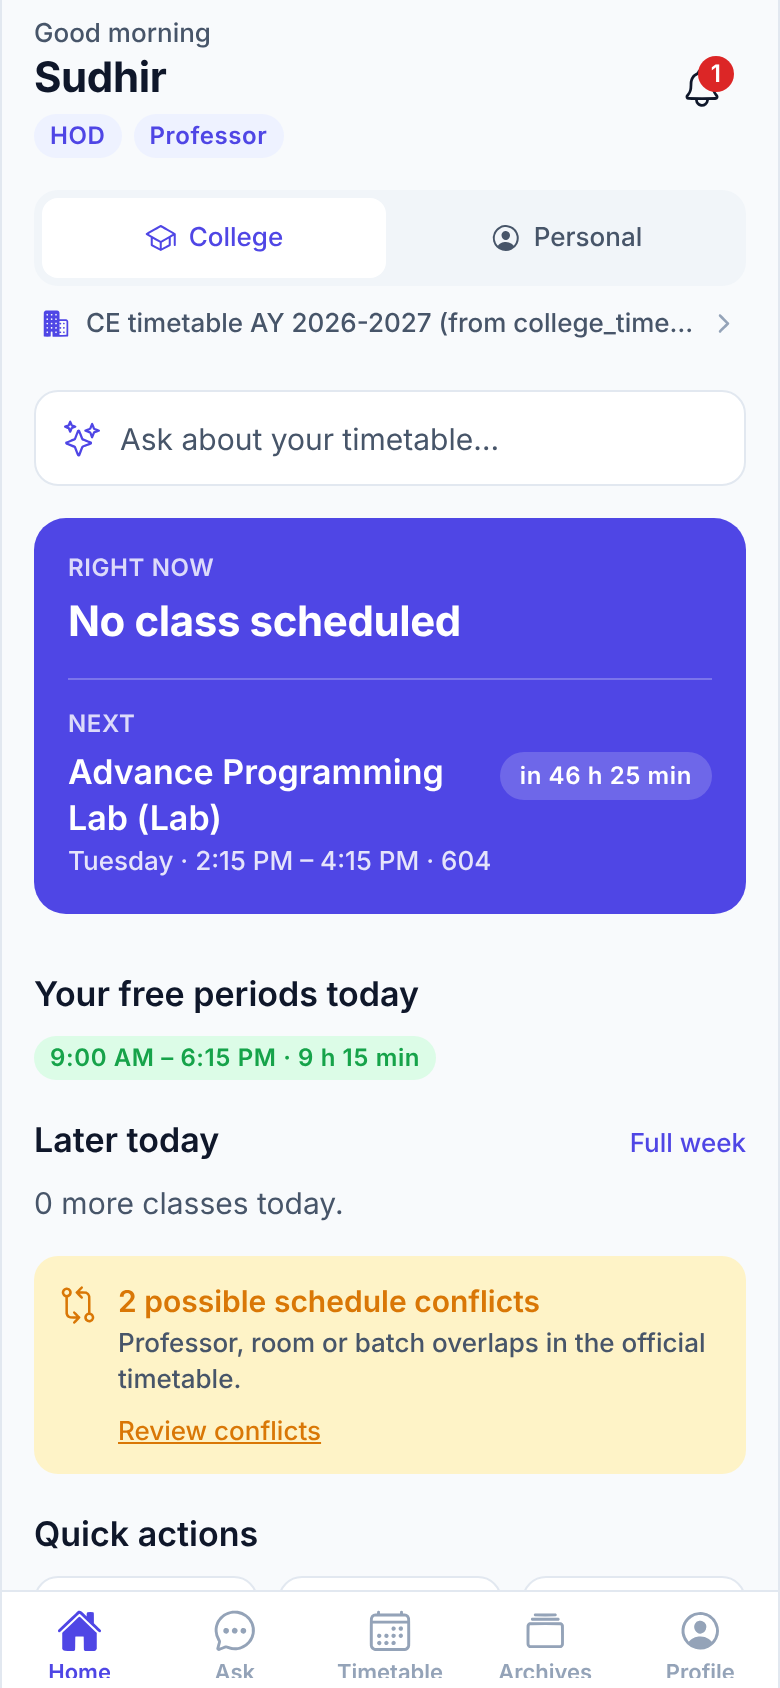
\includegraphics[width=\linewidth]{figures/screens/hod-home.png}\caption{HOD home with conflict alert}\end{subfigure}\hfill
\begin{subfigure}[t]{0.24\textwidth}\centering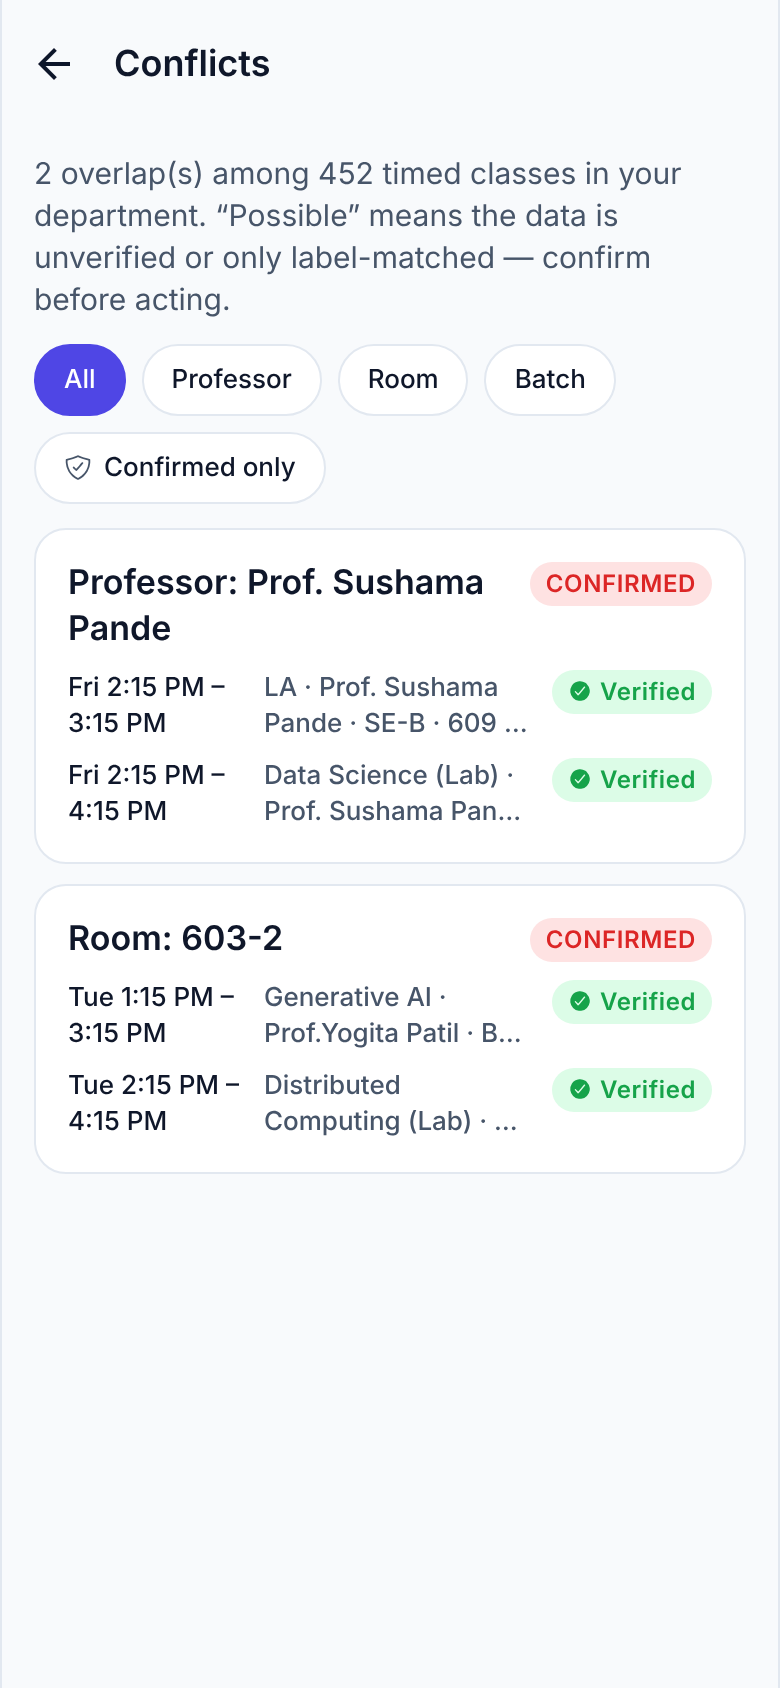
\includegraphics[width=\linewidth]{figures/screens/conflicts.png}\caption{The 2 genuine clashes}\end{subfigure}\hfill
\begin{subfigure}[t]{0.24\textwidth}\centering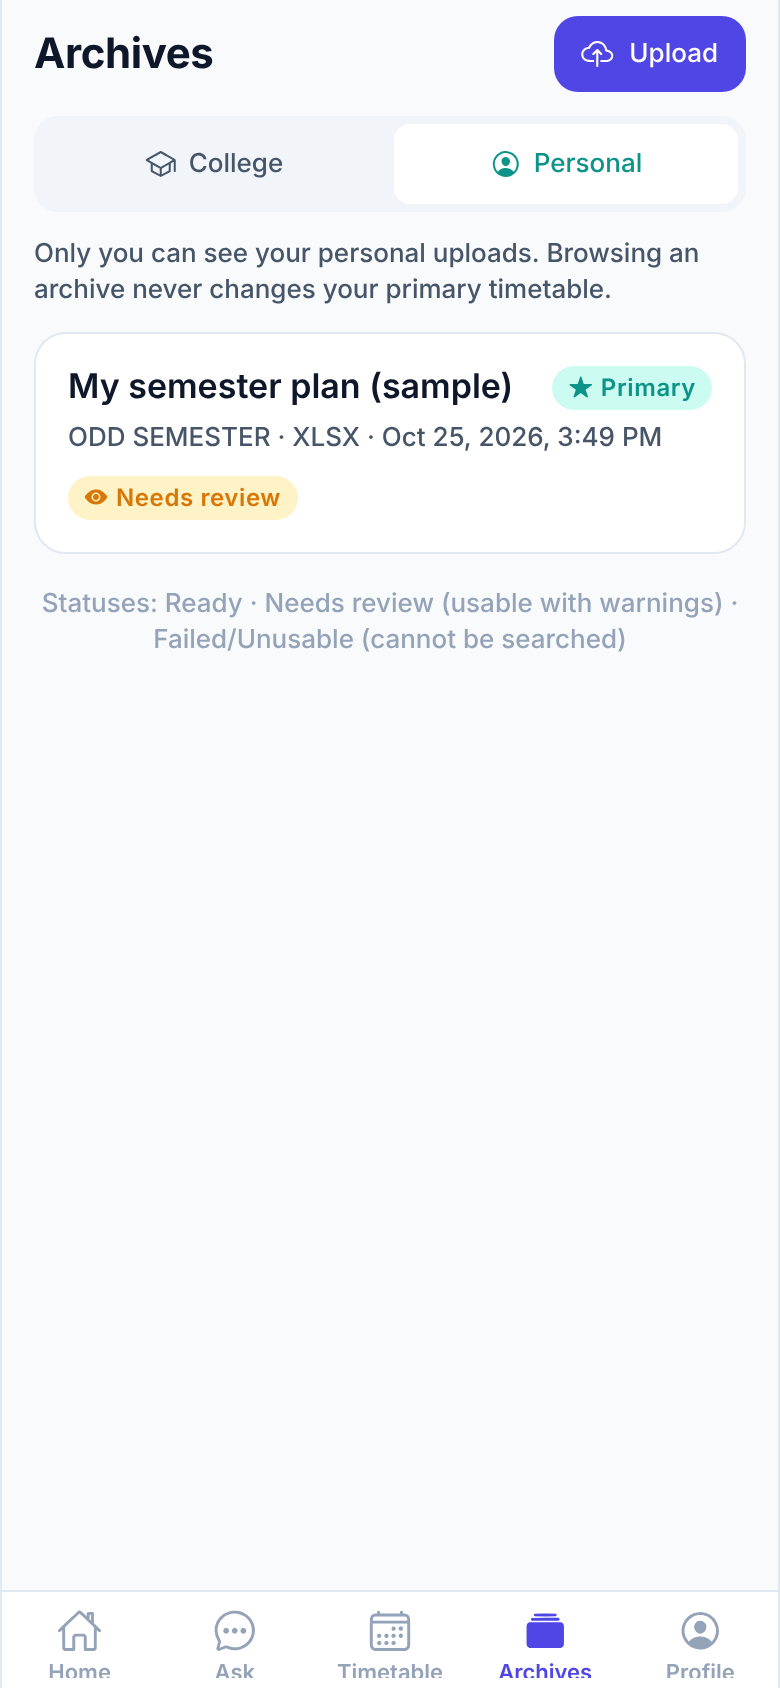
\includegraphics[width=\linewidth]{figures/screens/personal-archives.png}\caption{Personal archives (private)}\end{subfigure}
\caption{Combined classes, HOD view, conflicts and personal domain}
\label{fig:screens2}
\end{figure}

\begin{figure}[H]
\centering
\begin{subfigure}[t]{0.24\textwidth}\centering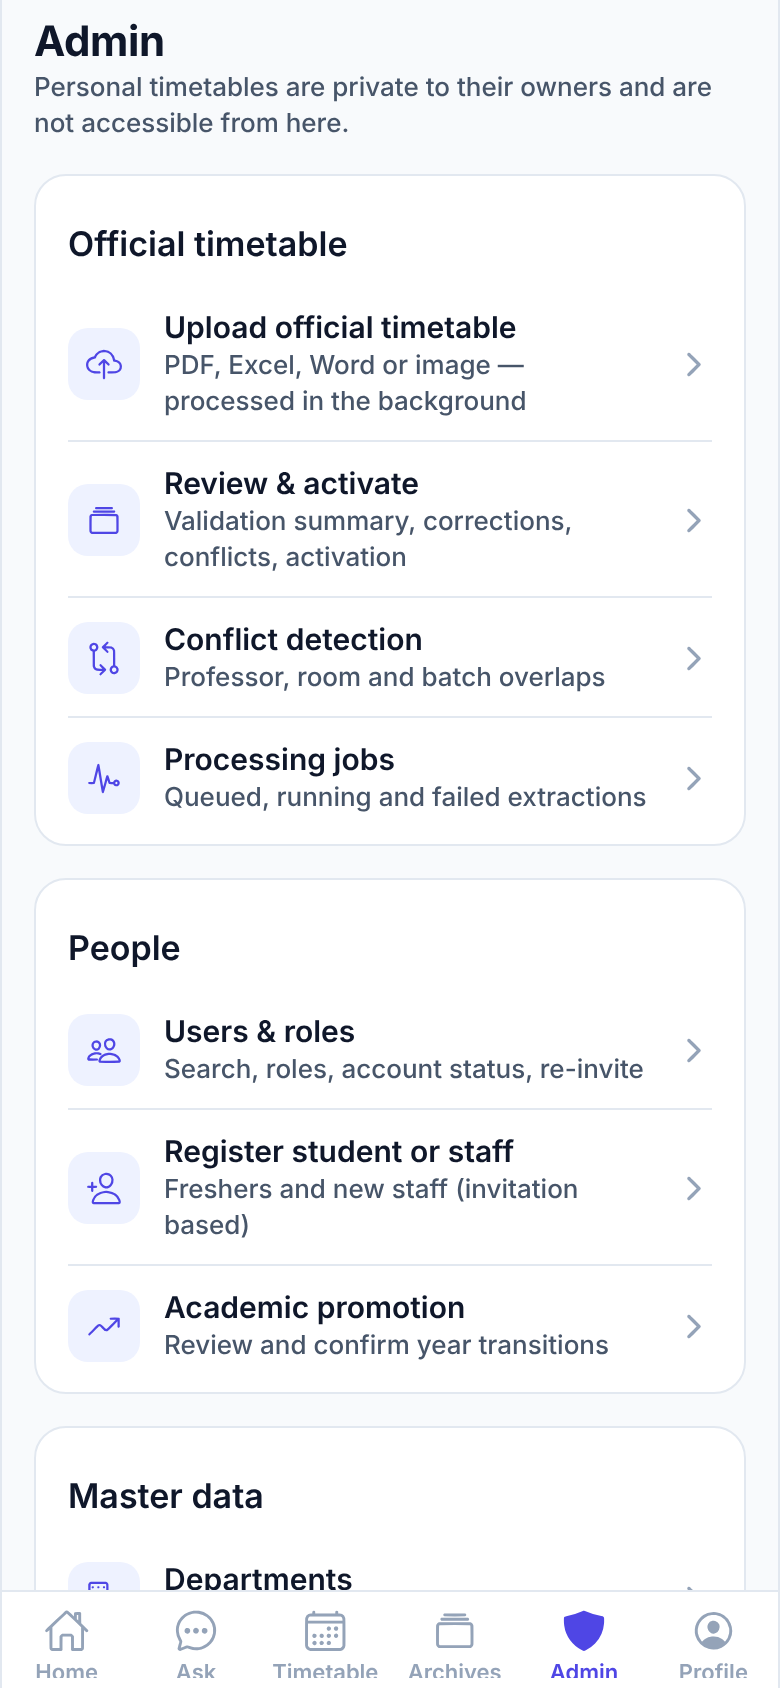
\includegraphics[width=\linewidth]{figures/screens/admin-hub.png}\caption{Admin hub}\end{subfigure}\hfill
\begin{subfigure}[t]{0.24\textwidth}\centering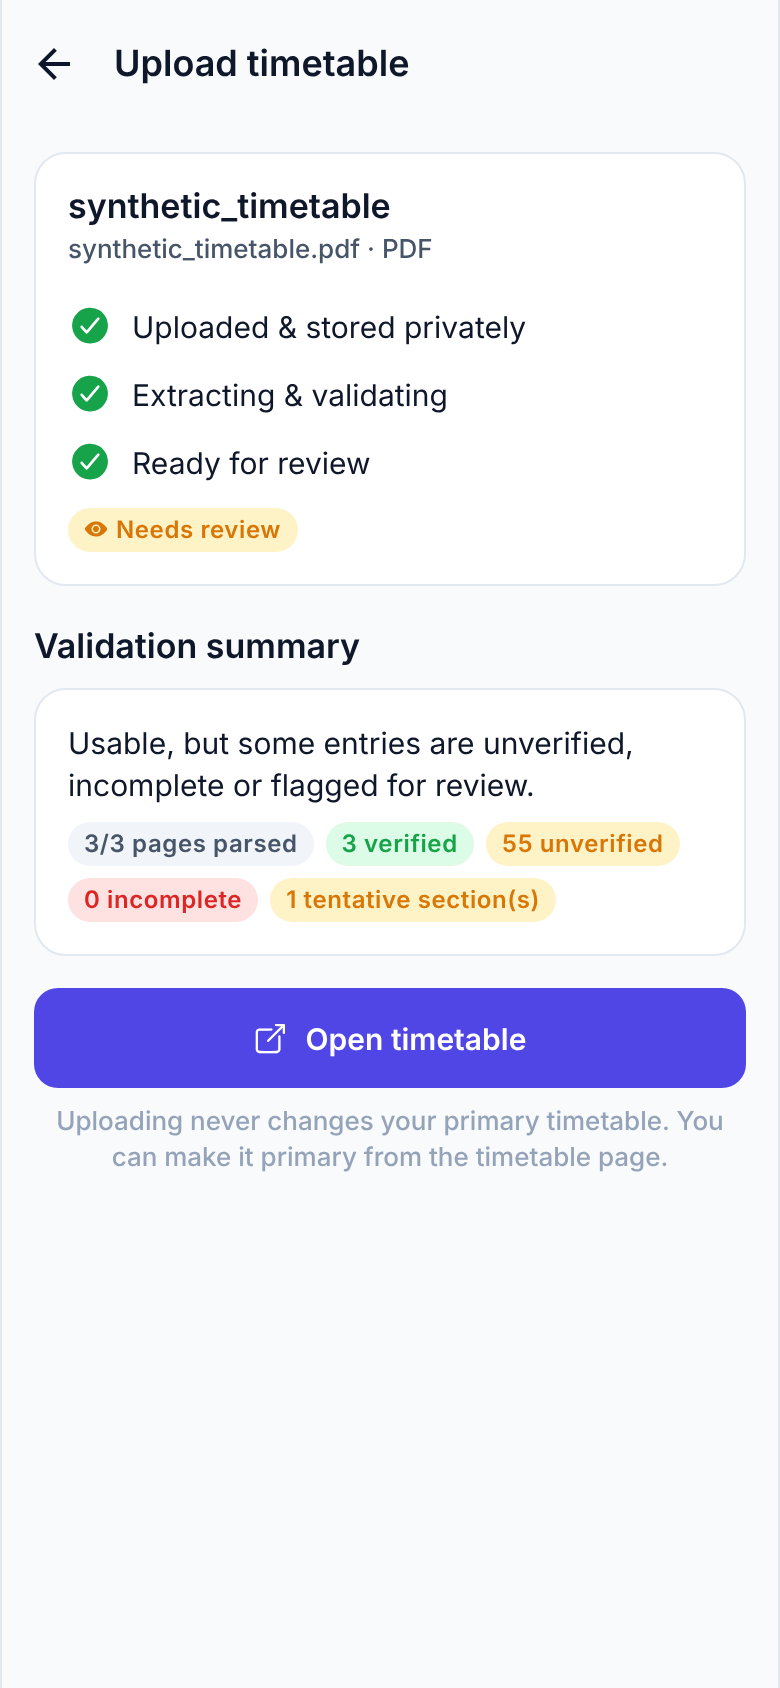
\includegraphics[width=\linewidth]{figures/screens/upload-processed.png}\caption{Upload processed by worker}\end{subfigure}\hfill
\begin{subfigure}[t]{0.24\textwidth}\centering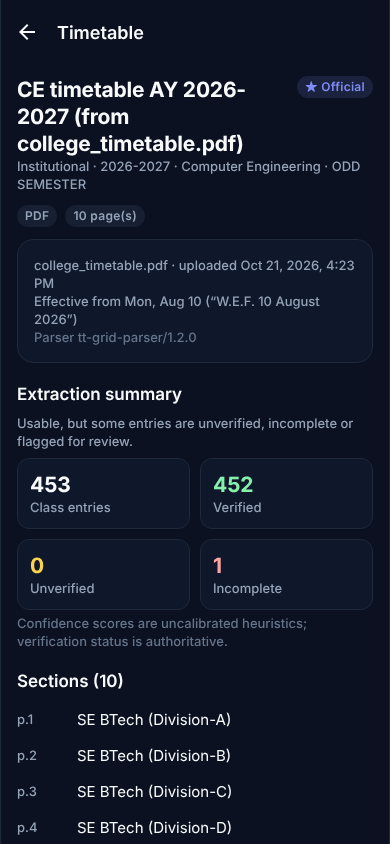
\includegraphics[width=\linewidth]{figures/screens/real-timetable-summary.png}\caption{Real PDF: 453 entries, 452 verified, 10 sections}\end{subfigure}
\caption{Administrator workflow}
\label{fig:screensadmin}
\end{figure}

\begin{figure}[H]
\centering
\begin{subfigure}[t]{0.31\textwidth}\centering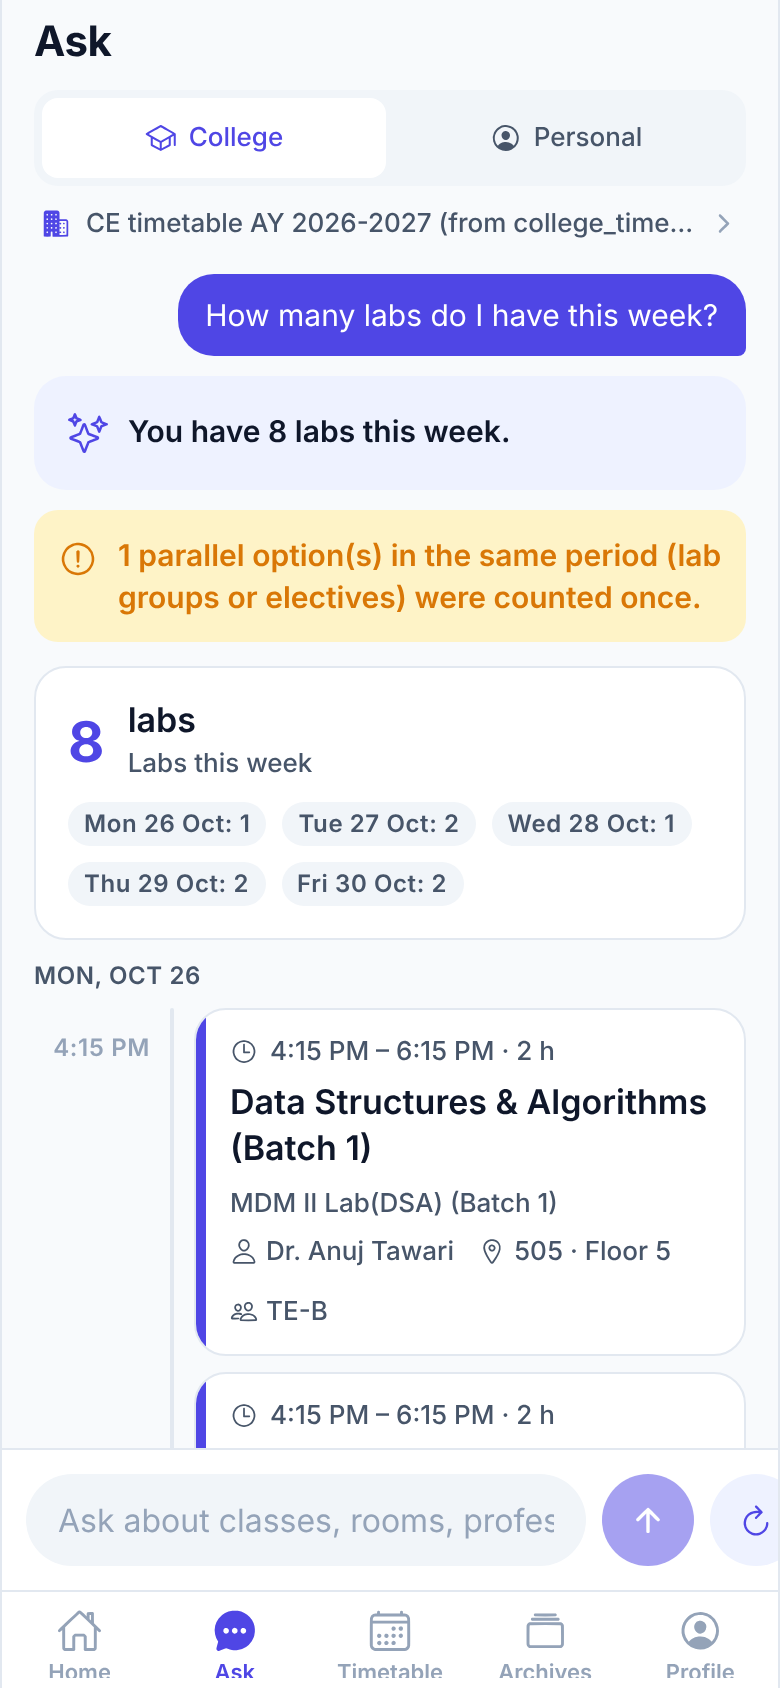
\includegraphics[width=\linewidth]{figures/screens/composed-count.png}\caption{``How many labs do I have this week?'': count with per-day breakdown}\end{subfigure}\hfill
\begin{subfigure}[t]{0.31\textwidth}\centering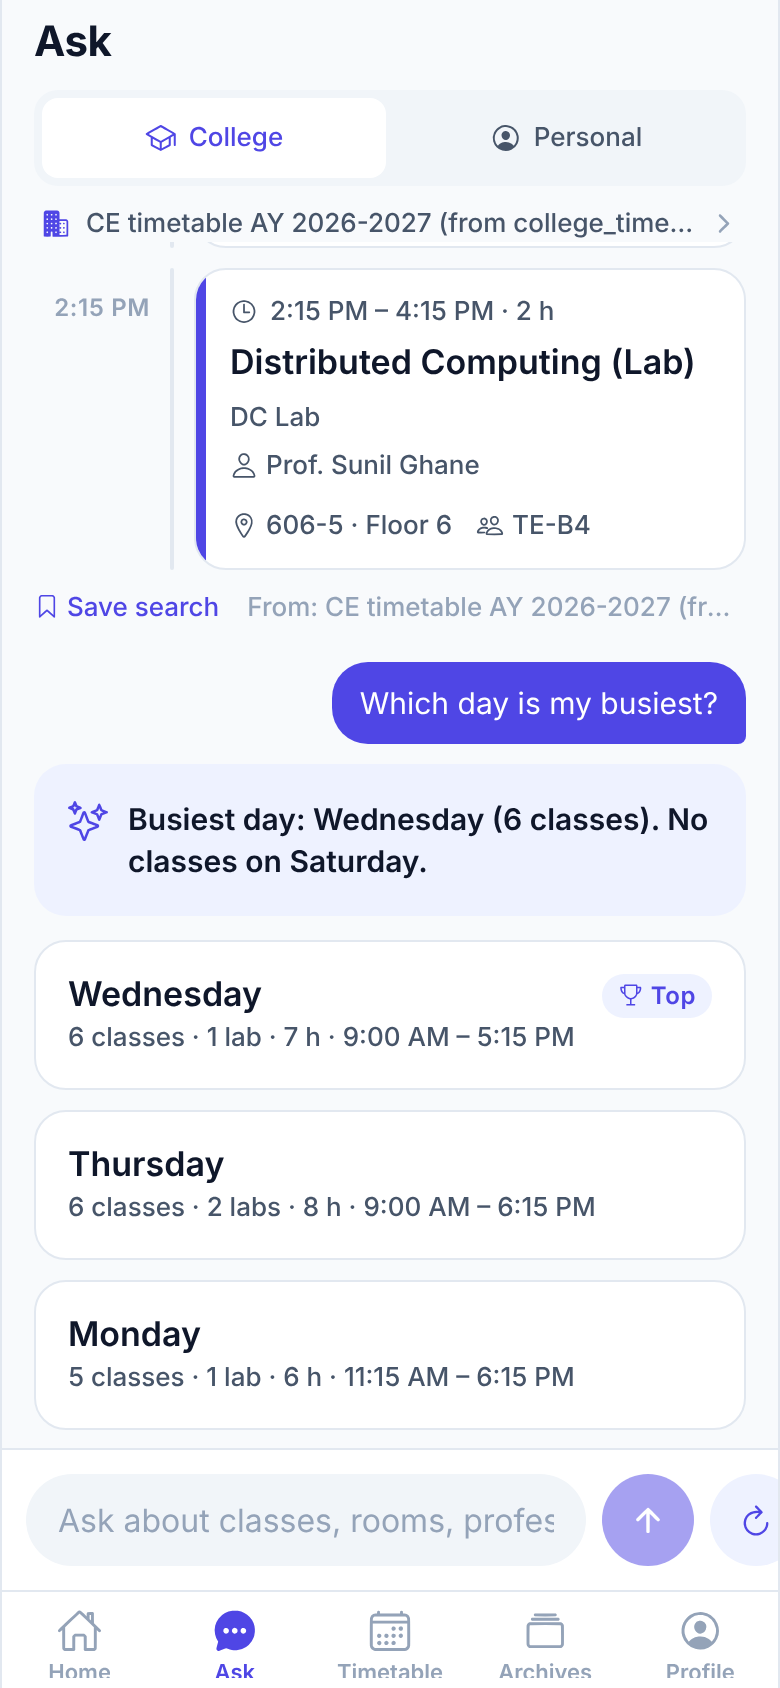
\includegraphics[width=\linewidth]{figures/screens/composed-busiest.png}\caption{``Which day is my busiest?'': day-wise summary}\end{subfigure}\hfill
\begin{subfigure}[t]{0.31\textwidth}\centering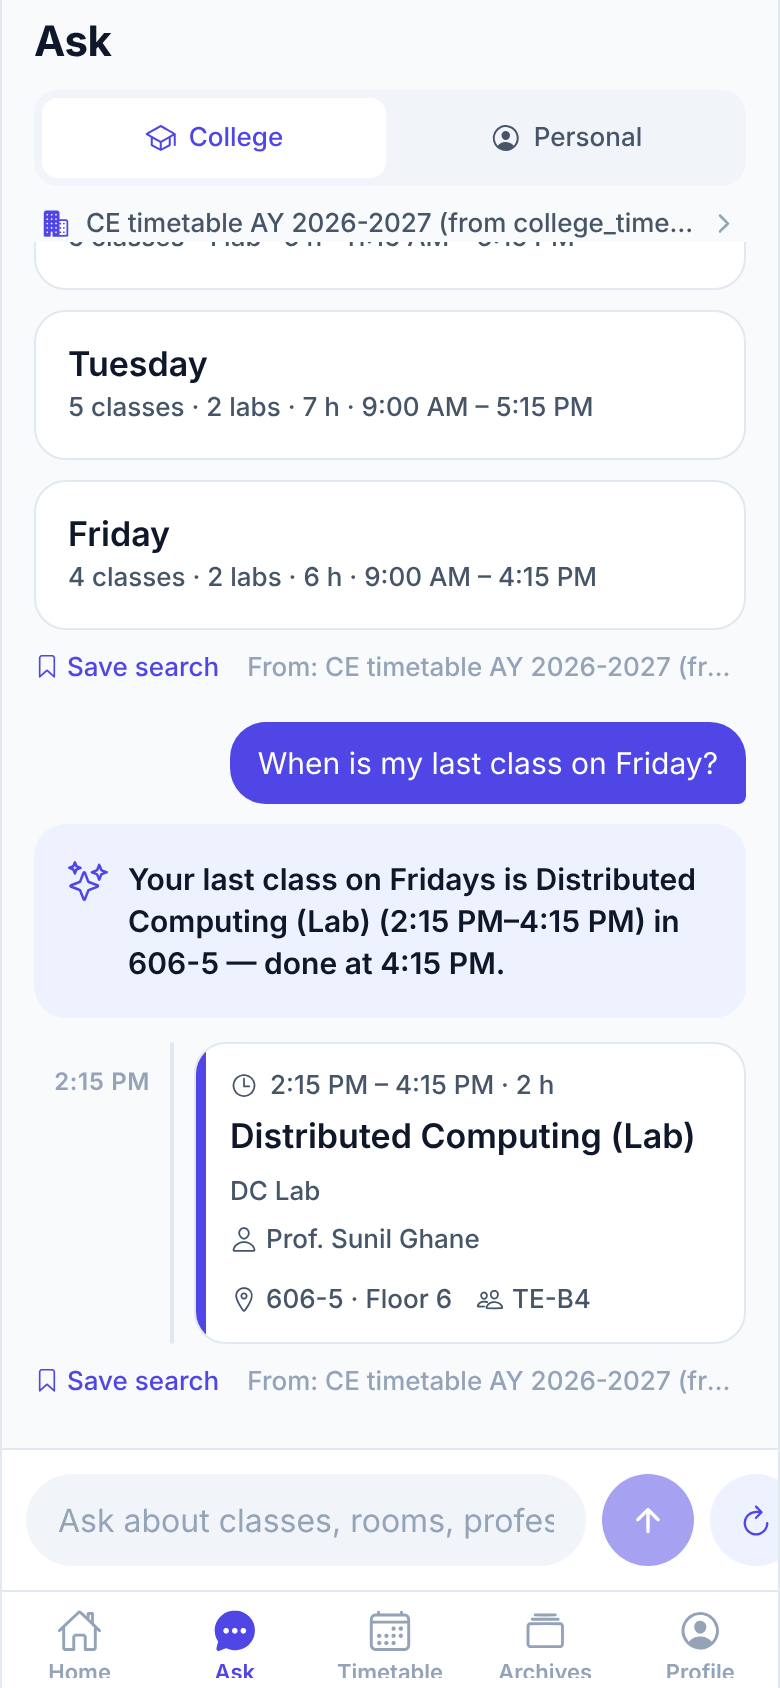
\includegraphics[width=\linewidth]{figures/screens/composed-last.png}\caption{``When is my last class on Friday?''}\end{subfigure}
\caption{Composed query plans answered from the real timetable (TE-B4 student)}
\label{fig:screenscomposed}
\end{figure}

\begin{figure}[H]
\centering
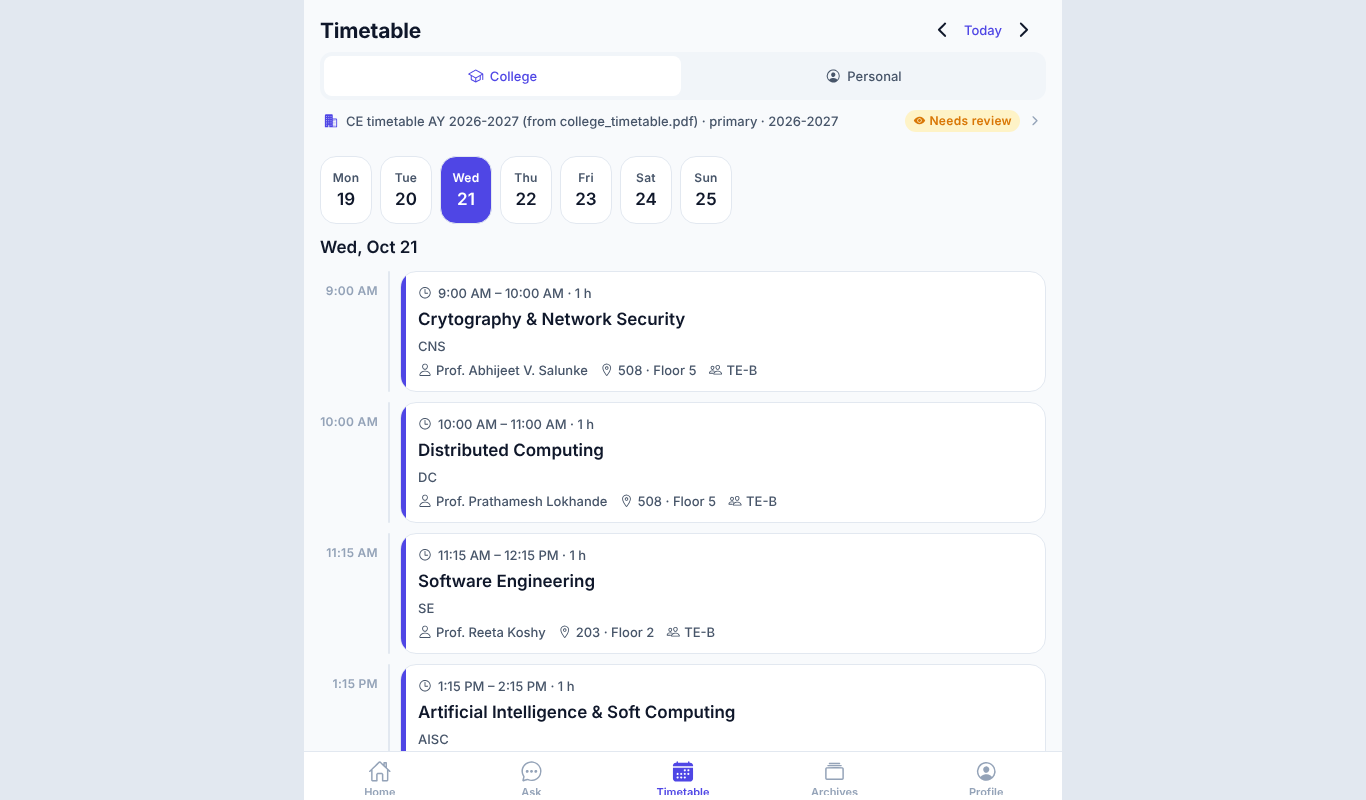
\includegraphics[width=0.8\textwidth]{figures/screens/laptop-timetable.png}
\caption{The same app in a laptop browser}
\label{fig:laptop}
\end{figure}

\subsection{Functional Results}
\begin{itemize}
\item \textbf{Extraction (FR-04):} the real PDF (10 pages, 420~kB) produced 570 rows: 453 class entries,
      of which \textbf{452 verified} and 1 \textsc{Incomplete} (M.Tech.\ HSS on Friday has no time
      label in the PDF), plus breaks and activities. All 10 pages were parsed, and 46 batches, 38
      courses, 52 faculty and 42 rooms were recognised.
\item \textbf{Conflicts (FR-13):} exactly two clashes, both confirmed by hand in the PDF:
      (1) \emph{Friday 2:15--3:15}, Prof.\ Sushama Pande has \emph{LA} for SE-B in 609 (page 2) and
      \emph{Data Science Lab C3} for SE-C in 606-4 (page 3); (2) \emph{Tuesday 2:15--3:15}, room
      \textbf{603-2} has B.E.\ \emph{PE III -- Gen AI} (page 9) and TE-D \emph{DC Lab D2} (page 8).
\item \textbf{Role views (FR-09/10):} SE-A1 sees only A1's labs on Wednesday; B.E.\ A and C both see
      the combined B.E.\ electives; LLC appears without teacher or room; the noon row 12:15--13:15 is a
      normal class.
\item \textbf{Queries (FR-11):} ``Do I have classes after lunch?'' uses 14:15 for S.E.\ and 13:15
      for T.E.\ (each from its own section). ``Am I free at 2?'' asks a.m./p.m. A student without a
      batch gets a setup message instead of an invented answer.
\item \textbf{Privacy (FR-14):} another user's personal timetable returns 404, even for the Admin.
\end{itemize}

\subsection{Performance Results}
Summarised from Chapter~8: median search latency 37--47~ms for a single user; 46.5~req/s at 4
clients and about 55--60~req/s at saturation with 4 workers on a 4-core VM; 0 wrong answers in 960
requests at 32 clients; extraction of the 10-page PDF in 1.65~s using 82~MB peak memory; 12~MB
database.

\begin{figure}[H]
\centering
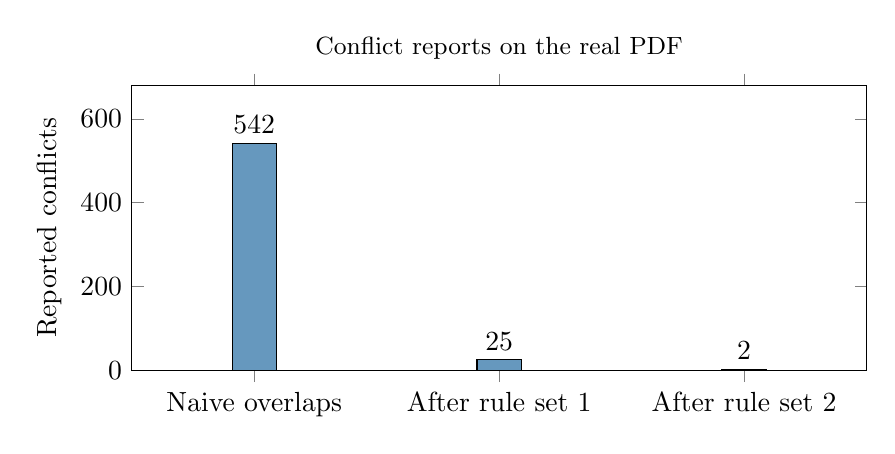
\begin{tikzpicture}
\begin{axis}[ybar,width=0.9\textwidth,height=5.2cm,bar width=16pt,ymin=0,ymax=680,
  symbolic x coords={Naive overlaps,After rule set 1,After rule set 2},xtick=data,
  nodes near coords,ylabel={Reported conflicts},enlarge x limits=0.25,title={\small Conflict reports on the real PDF}]
\addplot[fill=spitblue!60] coordinates {(Naive overlaps,542) (After rule set 1,25) (After rule set 2,2)};
\end{axis}
\end{tikzpicture}
\caption{Effect of intended-overlap rules: from 542 raw overlaps to the 2 genuine clashes}
\label{fig:conflictbar}
\end{figure}

\subsection{Comparison with Existing Systems}
Using the criteria of Table~\ref{tab:compare}, the proposed system is the only one that reads the
published timetable and also answers role-scoped questions safely. Table~\ref{tab:effort} compares
the effort for common tasks. The manual times are our own estimates from trying each task with the PDF;
they were not measured in a controlled study.

\begin{table}[H]
\centering
\caption{Task effort: manual PDF lookup vs.\ the app (manual times are estimates)}
\label{tab:effort}
\small
\begin{tabularx}{\textwidth}{@{}Xp{3.5cm}p{3.5cm}@{}}
\toprule
\textbf{Task} & \textbf{Manual PDF} & \textbf{Dynamic Timetable}\\
\midrule
Find my next class and its room & find page, row, column, lab group, legend: about 1 min & open app: 0 taps\\
Find a free room at 11~am on floor 6 & check every page for every room: 10+ min & one question, $<$1 s\\
Check all teacher/room clashes & impractical by hand (453 classes) & automatic, on every upload\\
Know whether the timetable changed & compare two PDFs by eye & notification + archive\\
Lab-group view (A1 vs A2) & read the stacked cells carefully & filtered automatically\\
\bottomrule
\end{tabularx}
\end{table}

\subsection{Achievement of Objectives}
\begin{table}[H]
\centering
\caption{Objectives mapped to evidence}
\label{tab:objectives}
\small
\begin{tabularx}{\textwidth}{@{}p{0.8cm}Xp{1.9cm}@{}}
\toprule
\textbf{Obj.} & \textbf{Evidence} & \textbf{Status}\\
\midrule
O1 & 99.8\% verified on the real PDF; uncertain values flagged (TC-07, TC-09) & Achieved\\
O2 & PDF, scanned PDF/photo (OCR), XLSX/XLS, CSV, DOCX/DOC through one pipeline (TC-04, TC-10) & Achieved\\
O3 & Five roles, server-side policy, role tests (TC-03), dashboards (Fig.~\ref{fig:screens1}, \ref{fig:screens2}) & Achieved\\
O4 & Specialised operations plus composed query plans (counts, first/last, day-wise, lab/lecture), with clarification (TC-16--TC-19, TC-31--TC-34) & Achieved\\
O5 & 2 genuine clashes, 0 false reports (TC-21) & Achieved\\
O6 & Separate tables; IDOR and isolation tests (TC-22); archives & Achieved\\
O7 & p50 37--47 ms; 0 wrong answers at 32 clients (TC-28, TC-29) & Achieved (dev hardware)\\
O8 & Android/iPhone via Expo Go, laptop browser, Render demo & Achieved; store builds pending\\
O9 & 168 + 20 + 45 e2e steps passing & Achieved\\
\bottomrule
\end{tabularx}
\end{table}

\subsection{Discussion of Findings}
\begin{itemize}
\item \textbf{Real data is different from specifications.} Most of the extraction work went into
      conventions found only in the real PDF: the mislabelled noon row, codes missing from legends, LLC
      slots and combined B.E.\ pages. Testing on the real document from early on was decisive.
\item \textbf{Honest uncertainty builds trust.} Marking the one entry without a time as
      \textsc{Incomplete}, instead of guessing, kept every automatic answer correct.
\item \textbf{The source document itself had errors.} The two clashes are real errors in the
      published timetable, so the system already adds value for the timetable committee.
\item \textbf{Unexpected observation:} a small connectivity check (\texttt{HEAD /}) made the whole
      production web app appear offline. This shows why end-to-end tests in a production-like
      configuration matter.
\item \textbf{Rules beat a black box here, if they compose.} A fixed list of question types felt limiting
      (counts, ``busiest day'', ``last lab on Friday'' were refused). Making the rules compose into a query
      plan removed most of that limit while keeping reproducible answers in about 40~ms, no API cost and
      no injection risk.
\end{itemize}

\subsection{Practical Applicability}
The department can use the system as it is for the current semester: the Admin uploads the
official PDF, reviews the flagged entry, activates it, and students and faculty use the web link
or the app. Before full-college use, the college should provide always-on hosting, e-mail for account
activation, and store builds of the app (Section~11.5). The approach also transfers to other
departments and institutes that publish grid-style timetables. Their layouts may need parser
adjustments, which the review workflow and regression tests are designed for.

\newpage

\section{Conclusion and Future Scope}

\subsection{Conclusion}
The college timetable is consulted by everyone every day, yet it exists only as a dense PDF that has
to be read by hand, with no search, no personal view, no version control and no clash checking. This
mini project built \emph{Dynamic Timetable}, a role-based timetable monitoring system that reads the
timetable as it is actually published (PDF, scanned image, Excel or Word), extracts every class with
its source page and a verification status, detects clashes, and serves students, professors, the HOD,
the Principal and the Admin through one app on Android, iPhone and laptop. Users can ask everyday
questions in plain English. A deterministic compositional planner turns each question into a typed
query plan (operation, filters, lab/lecture, date or week, time window, ordering) and compiles it into
parameterised queries, so it answers counts, first/last and day-wise questions as well as the everyday
ones in about 40~ms, never generates SQL from text, and asks for clarification instead of guessing. On the college's real 10-page timetable the system verified 452 of 453 class entries
automatically and found the two genuine clashes in the published document. The system is covered by
168 back-end tests, 20 app tests and end-to-end browser tests, and it runs as a free online demo.

\subsection{Achievement of Objectives}
\begin{itemize}
\item \textbf{Achieved:} O1 (99.8\% verified), O2 (all formats through one pipeline), O3 (five roles,
      server-side), O4 (composed query plans plus specialised operations), O5 (0 false clash reports), O6 (strict domain separation and
      archives), O9 (all tests passing).
\item \textbf{Achieved on development hardware:} O7 (latency and correctness under 32 concurrent
      clients). It still has to be confirmed on production hardware.
\item \textbf{Partially achieved:} O8. The app runs on Android and iPhone through Expo Go and on
      laptops through the web and the online demo, but installable store builds (APK/TestFlight) have
      not yet been produced.
\end{itemize}

\subsection{Major Engineering Contributions}
\begin{enumerate}
\item A timetable-aware extraction pipeline with constrained backtracking for inconsistent time labels,
      stacked lab-group parsing, page-local legends and per-entry provenance.
\item A conflict detector that separates intended overlaps (parallel labs, electives, shared sessions)
      from genuine clashes in $O(n\log n + m)$.
\item A safe, compositional natural-language interface: questions become typed query plans (operation,
      filters, lab/lecture, date or week, time window, ordering) compiled into parameterised queries with
      timetable-scoped entity resolution and clarification instead of guessing, injection-proof by design
      and no longer limited to a fixed list of questions.
\item A secure multi-role architecture: Argon2id, rotating refresh tokens with reuse detection,
      database-level ownership constraints (composite FKs, partial unique indexes) and audited corrections.
\item A free, reproducible deployment: Docker image, infrastructure as code (\texttt{render.yaml}) and
      continuous deployment from Git.
\end{enumerate}

\subsection{Current Limitations}
\begin{itemize}
\item \textbf{Technical:} extraction accuracy has not been measured against a hand-labelled ground truth;
      new timetable layouts may need parser rules; the rate limiter is per process; co-taught cells
      (``RRS+SB'') are not linked to both teachers' personal schedules.
\item \textbf{Functional:} the system does not generate timetables; questions outside the 30
      intents are politely refused; teacher location is the \emph{scheduled} room, not tracked.
\item \textbf{Operational:} the free demo sleeps when idle and its database expires every 30 days;
      push notifications and e-mail are not yet active; room floors were derived from room numbers and
      must be checked by the Admin.
\end{itemize}

\subsection{Future Enhancements}
\begin{enumerate}
\item Measure precision/recall on hand-labelled pages and publish per-field accuracy.
\item College single sign-on (OIDC/Google Workspace) instead of separate passwords.
\item Store builds (Android APK / Play Store, iOS TestFlight) with push notifications for timetable
      changes and ``class starting in 10 minutes'' reminders.
\item ``What changed?'' diff between two official versions, sent to affected users only.
\item Bulk CSV import of students, staff and rooms; many-to-many teacher links for co-taught classes.
\item An optional LLM \emph{suggester} that proposes an intent and parameters for unusual phrasings,
      which must still pass the same validation and templates (never free SQL).
\item Room-utilisation analytics for the HOD and Principal; exam-timetable support.
\item Capacity testing on production hardware; a shared rate-limit store and vocabulary caching for
      multi-instance deployment.
\end{enumerate}

\subsection{Lessons Learned}
\begin{itemize}
\item \textbf{Test with real data early.} The real PDF broke assumptions that synthetic data never would.
\item \textbf{Make uncertainty visible.} Statuses, raw text and page numbers turned possible silent
      errors into review tasks.
\item \textbf{Security is a design decision.} Choosing templates over generated SQL removed a whole
      class of attacks; our own audit still found a critical bug (P0-1), which showed us the value of reviewing our own code adversarially.
\item \textbf{Automated tests make change safe.} The SDK upgrade and the parser changes were made with
      confidence because 200+ tests guarded behaviour.
\item \textbf{Project management:} risk-first ordering (extraction before UI), small increments,
      one commit per working increment, and documenting decisions (why, not only what) kept the
      project on schedule and easy to explain.
\end{itemize}

\newpage


\newpage
\phantomsection\addcontentsline{toc}{section}{References}
% IEEE-style numbered references (one consistent style, ordered by first citation is not required;
% the list is grouped: research papers, standards, books, tools and documentation).
\begin{thebibliography}{99}

\bibitem{schaerf1999}
A.~Schaerf, ``A survey of automated timetabling,'' \emph{Artificial Intelligence Review}, vol.~13,
no.~2, pp.~87--127, 1999.

\bibitem{burke2002}
E.~K. Burke and S.~Petrovic, ``Recent research directions in automated timetabling,''
\emph{European Journal of Operational Research}, vol.~140, no.~2, pp.~266--280, 2002.

\bibitem{lewis2008}
R.~Lewis, ``A survey of metaheuristic-based techniques for university timetabling problems,''
\emph{OR Spectrum}, vol.~30, no.~1, pp.~167--190, 2008.

\bibitem{zanibbi2004}
R.~Zanibbi, D.~Blostein and J.~R. Cordy, ``A survey of table recognition: Models, observations,
transformations, and inferences,'' \emph{International Journal on Document Analysis and Recognition},
vol.~7, no.~1, pp.~1--16, 2004.

\bibitem{kieninger1998}
T.~Kieninger and A.~Dengel, ``The T-Recs table recognition and analysis system,'' in
\emph{Document Analysis Systems: Theory and Practice (DAS'98)}, LNCS vol.~1655, Springer, 1999,
pp.~255--270.

\bibitem{gobel2013}
M.~G\"obel, T.~Hassan, E.~Oro and G.~Orsi, ``ICDAR 2013 table competition,'' in \emph{Proc. 12th
International Conference on Document Analysis and Recognition (ICDAR)}, 2013, pp.~1449--1453.

\bibitem{smith2007}
R.~Smith, ``An overview of the Tesseract OCR engine,'' in \emph{Proc. 9th International Conference on
Document Analysis and Recognition (ICDAR)}, 2007, pp.~629--633.

\bibitem{androutsopoulos1995}
I.~Androutsopoulos, G.~D. Ritchie and P.~Thanisch, ``Natural language interfaces to databases --
an introduction,'' \emph{Natural Language Engineering}, vol.~1, no.~1, pp.~29--81, 1995.

\bibitem{zhong2017}
V.~Zhong, C.~Xiong and R.~Socher, ``Seq2SQL: Generating structured queries from natural language
using reinforcement learning,'' \emph{arXiv preprint arXiv:1709.00103}, 2017.

\bibitem{yu2018}
T.~Yu \emph{et al.}, ``Spider: A large-scale human-labeled dataset for complex and cross-domain
semantic parsing and text-to-SQL task,'' in \emph{Proc. Conference on Empirical Methods in Natural
Language Processing (EMNLP)}, 2018, pp.~3911--3921.

\bibitem{greshake2023}
K.~Greshake, S.~Abdelnabi, S.~Mishra, C.~Endres, T.~Holz and M.~Fritz, ``Not what you've signed up
for: Compromising real-world LLM-integrated applications with indirect prompt injection,'' in
\emph{Proc. 16th ACM Workshop on Artificial Intelligence and Security (AISec)}, 2023, pp.~79--90.

\bibitem{pedro2023}
R.~Pedro, D.~Castro, P.~Carreira and N.~Santos, ``From prompt injections to SQL injection attacks:
How protected is your LLM-integrated web application?,'' \emph{arXiv preprint arXiv:2308.01990}, 2023.

\bibitem{allen1983}
J.~F. Allen, ``Maintaining knowledge about temporal intervals,'' \emph{Communications of the ACM},
vol.~26, no.~11, pp.~832--843, 1983.

\bibitem{sandhu1996}
R.~S. Sandhu, E.~J. Coyne, H.~L. Feinstein and C.~E. Youman, ``Role-based access control models,''
\emph{IEEE Computer}, vol.~29, no.~2, pp.~38--47, 1996.

\bibitem{biryukov2016}
A.~Biryukov, D.~Dinu and D.~Khovratovich, ``Argon2: New generation of memory-hard functions for
password hashing and other applications,'' in \emph{Proc. IEEE European Symposium on Security and
Privacy (EuroS\&P)}, 2016, pp.~292--302.

\bibitem{fielding2000}
R.~T. Fielding, ``Architectural styles and the design of network-based software architectures,''
Ph.D. dissertation, University of California, Irvine, 2000.

\bibitem{codd1970}
E.~F. Codd, ``A relational model of data for large shared data banks,'' \emph{Communications of the
ACM}, vol.~13, no.~6, pp.~377--387, 1970.

\bibitem{rfc7519}
M.~Jones, J.~Bradley and N.~Sakimura, ``JSON Web Token (JWT),'' IETF RFC~7519, May 2015.

\bibitem{owasp2021}
OWASP Foundation, ``OWASP Top 10:2021,'' 2021. [Online]. Available: https://owasp.org/Top10/

\bibitem{silberschatz2019}
A.~Silberschatz, H.~F. Korth and S.~Sudarshan, \emph{Database System Concepts}, 7th~ed.
New York: McGraw-Hill, 2019.

\bibitem{cormen2009}
T.~H. Cormen, C.~E. Leiserson, R.~L. Rivest and C.~Stein, \emph{Introduction to Algorithms},
3rd~ed. Cambridge, MA: MIT Press, 2009.

\bibitem{silberschatzos}
A.~Silberschatz, P.~B. Galvin and G.~Gagne, \emph{Operating System Concepts}, 10th~ed.
Hoboken, NJ: Wiley, 2018.

\bibitem{sommerville}
I.~Sommerville, \emph{Software Engineering}, 10th~ed. Boston: Pearson, 2016.

\bibitem{fet}
L.~Lalescu \emph{et al.}, ``FET -- Free Timetabling Software.'' [Online]. Available:
https://lalescu.ro/liviu/fet/

\bibitem{unitime}
UniTime, ``UniTime -- Comprehensive University Timetabling System.'' [Online]. Available:
https://www.unitime.org/

\bibitem{asc}
Applied Software Consultants, ``aSc Timetables.'' [Online]. Available: https://www.asctimetables.com/

\bibitem{tabula}
Tabula, ``Tabula: Extract tables from PDFs.'' [Online]. Available: https://tabula.technology/

\bibitem{camelot}
Camelot, ``Camelot: PDF table extraction for humans.'' [Online]. Available:
https://camelot-py.readthedocs.io/

\bibitem{pymupdf}
Artifex Software, ``PyMuPDF documentation.'' [Online]. Available: https://pymupdf.readthedocs.io/

\bibitem{postgresdocs}
The PostgreSQL Global Development Group, ``PostgreSQL 16 Documentation -- SELECT: The locking
clause (FOR UPDATE, SKIP LOCKED).'' [Online]. Available: https://www.postgresql.org/docs/16/sql-select.html

\bibitem{fastapi}
S.~Ram\'irez, ``FastAPI documentation.'' [Online]. Available: https://fastapi.tiangolo.com/

\bibitem{expo}
Expo, ``Expo documentation (SDK 58).'' [Online]. Available: https://docs.expo.dev/

\bibitem{reactnative}
Meta Platforms, ``React Native documentation.'' [Online]. Available: https://reactnative.dev/

\bibitem{render}
Render, ``Render documentation -- Free instance types and free PostgreSQL.'' [Online]. Available:
https://render.com/docs/free

\end{thebibliography}


\end{document}
